\ifdefined\ishandout
\documentclass[handout, 10pt]{beamer}
\else
\documentclass[10pt]{beamer}
\fi

%\usepackage[frenchb]{babel}
\usepackage[T1]{fontenc}
%\usepackage[utf8]{inputenc}
\usepackage{hyperref}
\usepackage{multirow}
\usepackage{listings}
\usepackage{fancyvrb}
\usepackage{tikz}
\usepackage{framed}
\usepackage{xmpmulti}
\usepackage{algorithm}
\usepackage{algorithmicx}
\usepackage{algpseudocode}
\usepackage{xcolor}
\usepackage{booktabs}
\usepackage{color, colortbl}
\ifdefined\ishandout
\usepackage{handoutWithNotes}
\fi
\usepackage{slashbox}
\usepackage{amsmath}
\usepackage{bm}
\usepackage{hhline}
\usepackage{pgfplots}
\usepackage{caption}
\graphicspath{{figs/}} %Setting the graphicspath

\usepackage[absolute,overlay]{textpos}
%\usepackage{graphicx}

\def\UrlBreaks{\do\/\do-}

\usetikzlibrary{shapes.geometric}
\usetikzlibrary{positioning}
\usetikzlibrary{shapes.arrows, chains}
\usetikzlibrary{arrows,calc}
\usetikzlibrary{shapes.multipart}
\usetikzlibrary{matrix}

\usepackage{array}
%\usetheme{Boadilla}
\usetheme[progressbar=frametitle]{metropolis}

\usefonttheme[onlymath]{serif}

\newcommand{\R}{\mathbb{R}}
%\newcommand{\C}{\mathbb{C}}
\newcommand{\N}{\mathbb{N}}
\newcommand{\Z}{\mathbb{Z}}
\newcommand{\E}{\mathbb{E}}
\newcommand{\Var}{\text{Var}}
\newcommand{\Cov}{\text{Cov}}
\ifdefined\ishandout
\pgfpagesuselayout{3 on 1 with notes}[a4paper,border shrink=5mm]
\usecolortheme{dove}
\else
%\usecolortheme{dolphin}
%\usecolortheme{crane}
\fi

\metroset{block=fill}

\lstnewenvironment{codeC}
{ \lstset{language=C,
    otherkeywords={printf,scanf}}
}
{}

\ifdefined\ishandout
\definecolor{mygreen}{rgb}{0,0,0}
\definecolor{mymauve}{rgb}{0,0,0}
\definecolor{myblue}{rgb}{0,0,0}
\else
\definecolor{mygreen}{rgb}{0,0.6,0}
\definecolor{mymauve}{rgb}{0.58,0,0.82}
\definecolor{myblue}{rgb}{0,0,1}

\fi

%% Notes
%\setbeameroption{show only notes}


\definecolor{mygray}{rgb}{0.5,0.5,0.5}

\lstset{ language=Python,%
  backgroundcolor=\color{white},   % choose the background color; you must add \usepackage{color} or \usepackage{xcolor}
  basicstyle=\footnotesize,        % the size of the fonts that are used for the code
  breakatwhitespace=false,         % sets if automatic breaks should only happen at whitespace
  breaklines=true,                 % sets automatic line breaking
  captionpos=b,                    % sets the caption-position to bottom
  commentstyle=\color{mygreen},    % comment style
  deletekeywords={...},            % if you want to delete keywords from the given language
  escapeinside={\%*}{*)},          % if you want to add LaTeX within your code
  extendedchars=true,              % lets you use non-ASCII characters; for 8-bits encodings only, does not work with UTF-8
  frame=tb,	                   % adds a frame around the code
  keepspaces=true,                 % keeps spaces in text, useful for keeping indentation of code (possibly needs columns=flexible)
  keywordstyle=\color{blue},       % keyword style
  otherkeywords={*,...},           % if you want to add more keywords to the set
  numbers=none,                    % where to put the line-numbers; possible values are (none, left, right)
  numbersep=5pt,                   % how far the line-numbers are from the code
  numberstyle=\tiny\color{mygray}, % the style that is used for the line-numbers
  rulecolor=\color{black},         % if not set, the frame-color may be changed on line-breaks within not-black text (e.g. comments (green here))
  showspaces=false,                % show spaces everywhere adding particular underscores; it overrides 'showstringspaces'
  showstringspaces=false,          % underline spaces within strings only
  showtabs=false,                  % show tabs within strings adding particular underscores
  stepnumber=2,                    % the step between two line-numbers. If it's 1, each line will be numbered
  stringstyle=\color{mymauve},     % string literal style
  tabsize=3,	                   % sets default tabsize to 2 spaces
  title=\lstname                   % show the filename of files included with \lstinputlisting; also try caption instead of title
}
%\lstset{language=Python,
% breakatwhitespace=false,         % sets if automatic breaks should only happen at whitespace
%  breaklines=true,                 % sets automatic line breaking
%  captionpos=b,                
%%commentstyle=\itshape\color{mymauve},
%%keywordstyle=\bfseries\color{myblue},
%numbers=left,                    % where to put the line-numbers; possible values are (none, left, right)
%  numbersep=8pt,                   % how far the line-numbers are from the code
%  numberstyle=\tiny\color{mygray}, % the style that is used for the line-numbers
%%  rulecolor=\color{black},         % if not set, the frame-color may be changed on line-breaks within not-black text (e.g. comments (green here))
%  showspaces=false,                % show spaces everywhere adding particular underscores; it overrides 'showstringspaces'
%%  showstringspaces=false,          % underline spaces within strings only
%  showtabs=false,                  % show tabs within strings adding particular underscores
%  stepnumber=2,                    % the step between two line-numbers. If it's 1, each line will be numbered
%%  stringstyle=\color{mygreen},     % string literal style
%  tabsize=2 
%}
\ifdefined\ishandout
\newcommand{\red}{\textbf}
\else
\newcommand{\red}{\textcolor{red}}
\fi
%\newcommand \emph
%Default size : 12.8 cm * 9.6 cm

\newcommand{\tmark}[1]{\tikz[remember picture, baseline=-.5ex]{\coordinate(#1);}}

\definecolor{bluegreen}{RGB}{0,149,182}


%\newcommand{\output}[1]{
\setbeamertemplate{navigation symbols}{}
\newcommand{\bvrb}{\Verb[commandchars=£µ§,formatcom=\color{bluegreen}]}
\newcommand{\footvrb}{\footnotesize\Verb}
\newcommand{\vrbalert}[2][]{\visible<#1>{#2}}
%%% Commande pour les listes/arbres
\newcommand{\mvide}{\nodepart{one} \nodepart{two}}
\newcommand{\tvide}{\nodepart{one} \nodepart{two} \nodepart{three}}
\newcommand{\rref}[1][]{\hfill{\scriptsize\textit{#1}}}

%%Fin des commandes pour les listes/arbres.



%%% Paramètres du cours (à régler)
%Numéro du cours
\newcommand{\nb}{1}

\title[Machine Learning]{Part 3: Random forest and Grid Search}
\author[A. Korosov]{anton.korosov@nersc.no}
\institute[NERSC]{NERSC\\
slides+notebook:\url{https://github.com/nansencenter/nersc_ml_course}}
\date{October 2021}

\begin{document}
\begin{frame}
\titlepage
\end{frame}

\begin{frame}[allowframebreaks]{Table of contents}
  \setbeamertemplate{section in toc}[sections numbered]
  \tableofcontents[hideallsubsections]
\end{frame}

\section{Regression problem and Classification probelm}

\begin{frame}{Regression}
\begin{textblock*}{8cm}(3cm,1cm) % {block width} (coords)
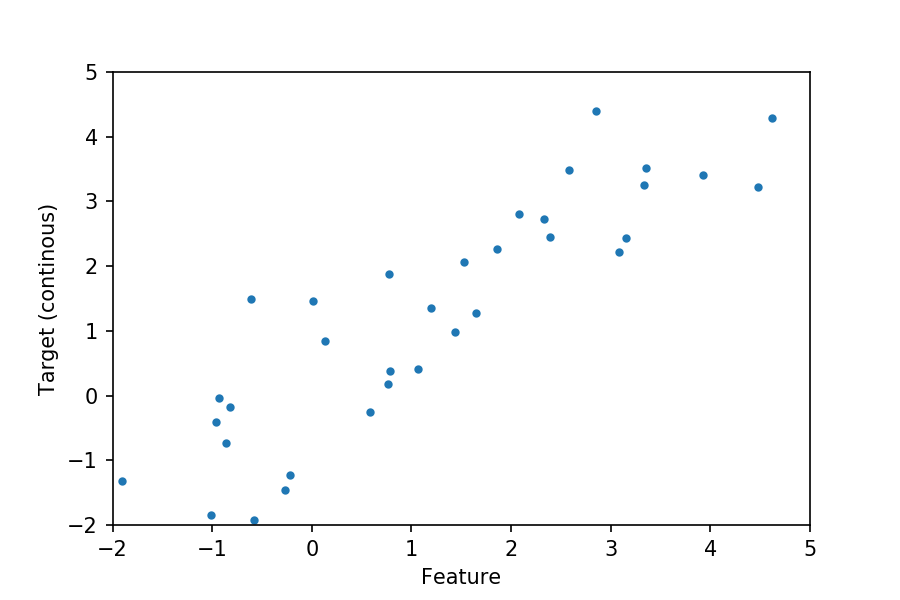
\includegraphics[width=7cm]{figs/regression_0.png}
\end{textblock*}
\end{frame}

\begin{frame}{Regression}
\begin{textblock*}{8cm}(3cm,1cm) % {block width} (coords)
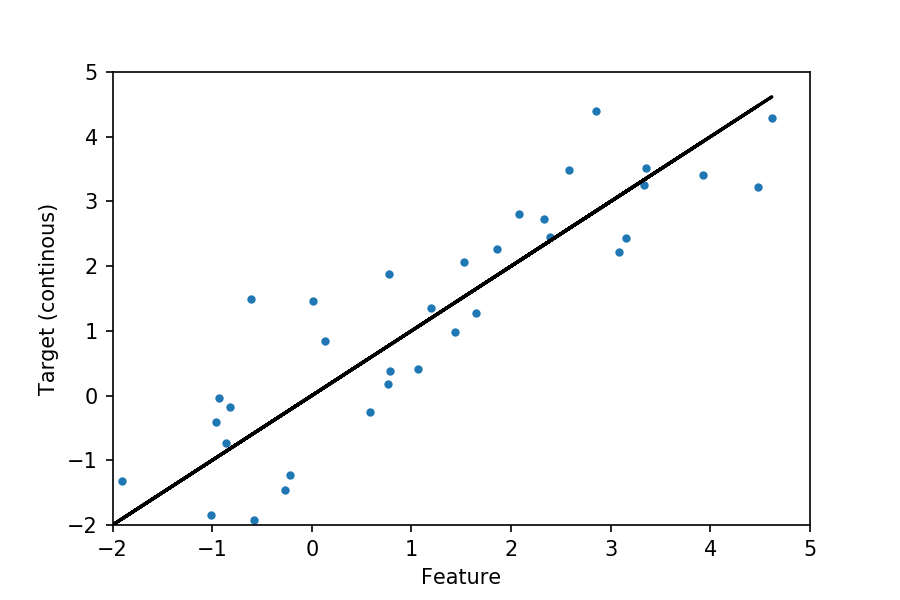
\includegraphics[width=7cm]{figs/regression_1.png}

Regression: the model links feature and a continuous target: 

$t = M(f)$
\end{textblock*}
\end{frame}

\begin{frame}{Regression}
\begin{textblock*}{8cm}(3cm,1cm) % {block width} (coords)
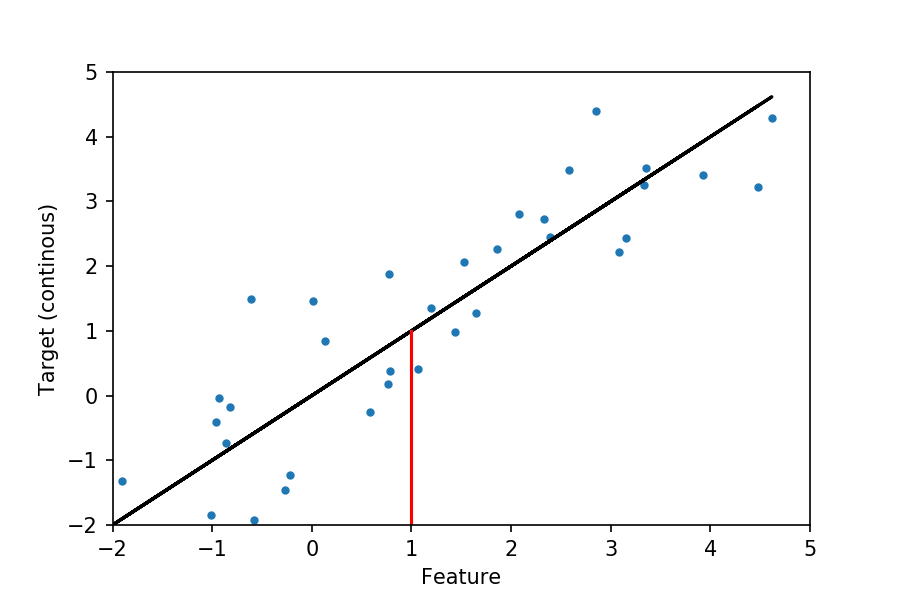
\includegraphics[width=7cm]{figs/regression_2.png}

If we have an unknown feature (x0 = 1): 
\end{textblock*}
\end{frame}

\begin{frame}{Regression}
\begin{textblock*}{8cm}(3cm,1cm) % {block width} (coords)
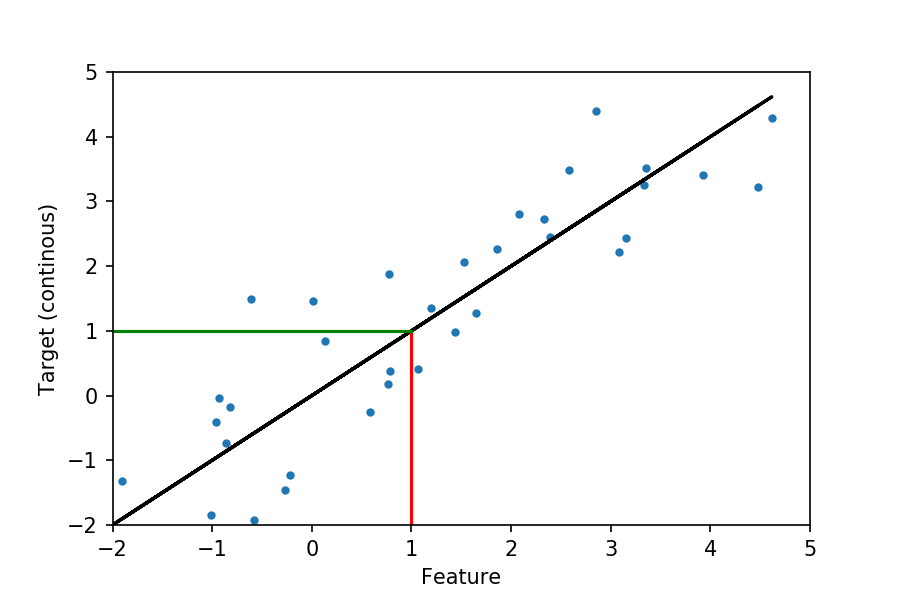
\includegraphics[width=7cm]{figs/regression_3.png}

We can compute a new target:

$t0 = M(x0)$
\end{textblock*}
\end{frame}

\begin{frame}{Classification}
\begin{textblock*}{8cm}(3cm,1cm) % {block width} (coords)
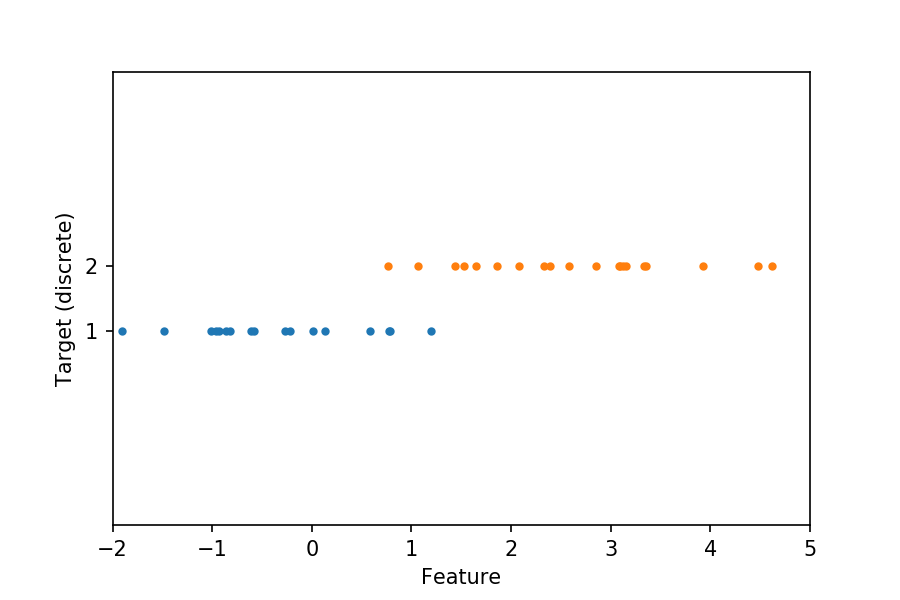
\includegraphics[width=7cm]{figs/classification_0.png}

Classification: for the same feature, the target is discrete. For example, only two classes.
\end{textblock*}
\end{frame}

\begin{frame}{Classification}
\begin{textblock*}{8cm}(3cm,1cm) % {block width} (coords)
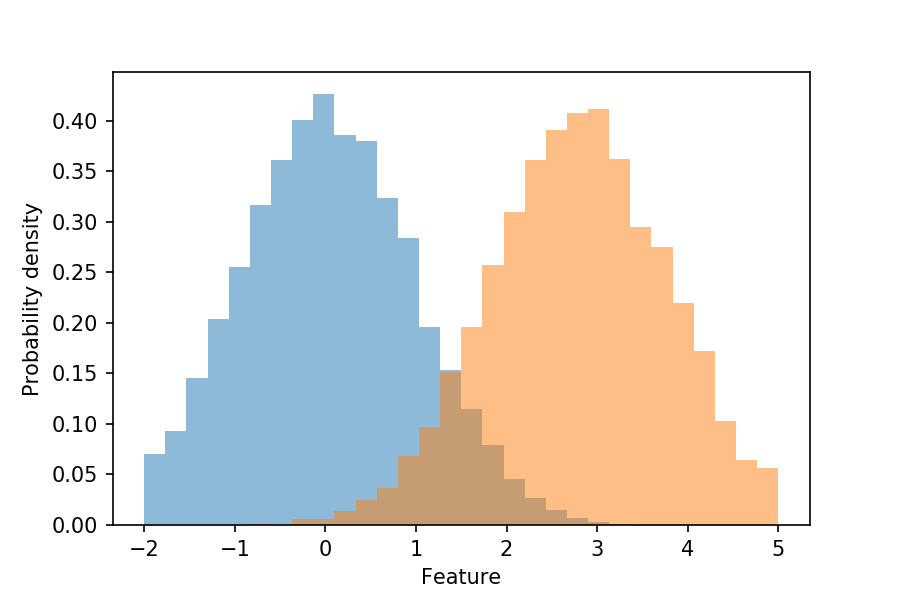
\includegraphics[width=7cm]{figs/classification_1.png}

The model links feature and target through probability. 

What are the probabilities of feature $f0$ to belong to classes $t0$ and $t1$?

$p_i = M(f)$
\end{textblock*}
\end{frame}

\begin{frame}{Classification}
\begin{textblock*}{8cm}(3cm,1cm) % {block width} (coords)
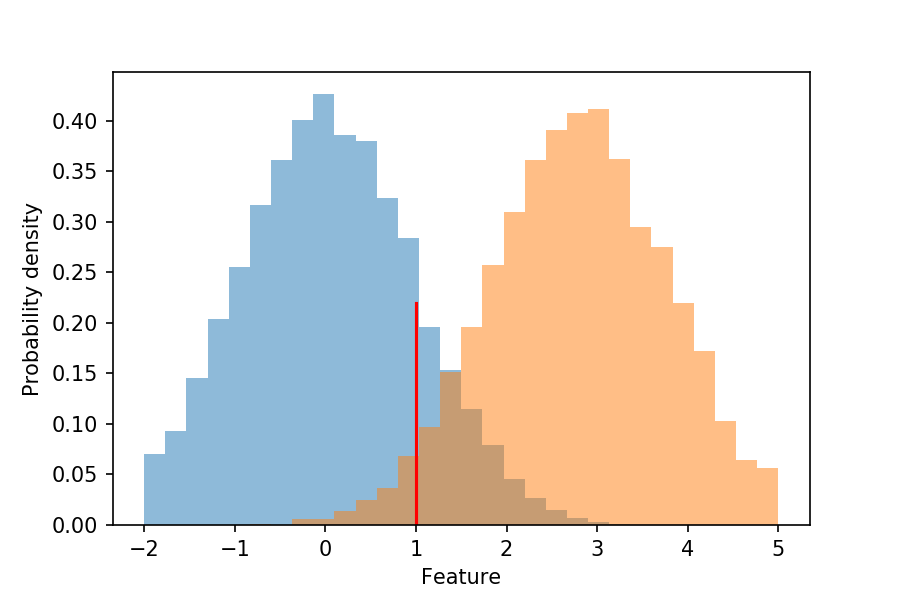
\includegraphics[width=7cm]{figs/classification_2.png}

Although the PDFs overlap, the probability that point $f=1$ belongs to class $p=1$ is higher. Therefore this point is classified as belonging to class 1.
\end{textblock*}
\end{frame}

\section{Decision trees}

\begin{frame}{Dataset: 20 points, 2 features x0 and x1, 2 classes}
\hspace*{-1cm}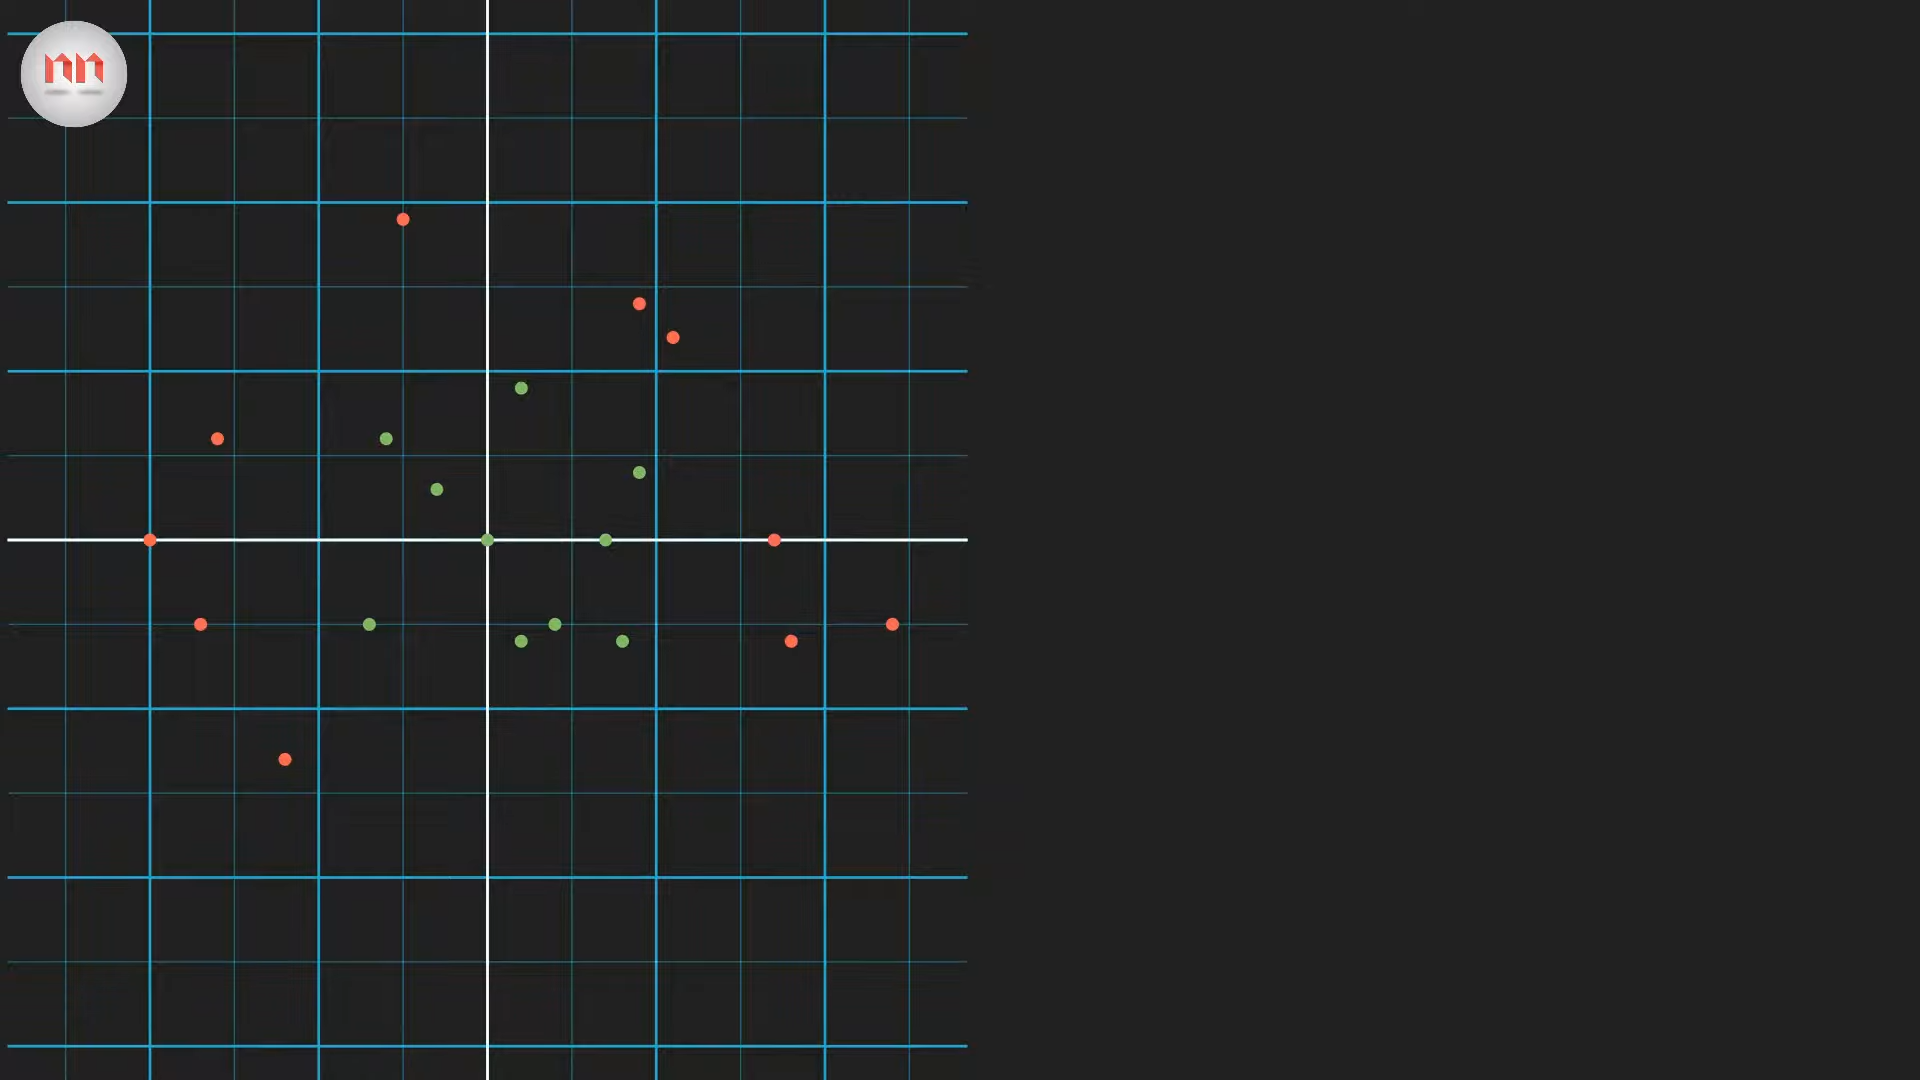
\includegraphics[width=13cm]{dt/_0-48 screenshot}
{\tiny \href{https://www.youtube.com/watch?v=ZVR2Way4nwQ}{ \copyright Normalized Nerd}}
\end{frame}

\begin{frame}{Decision tree ready for classification}
\hspace*{-1cm}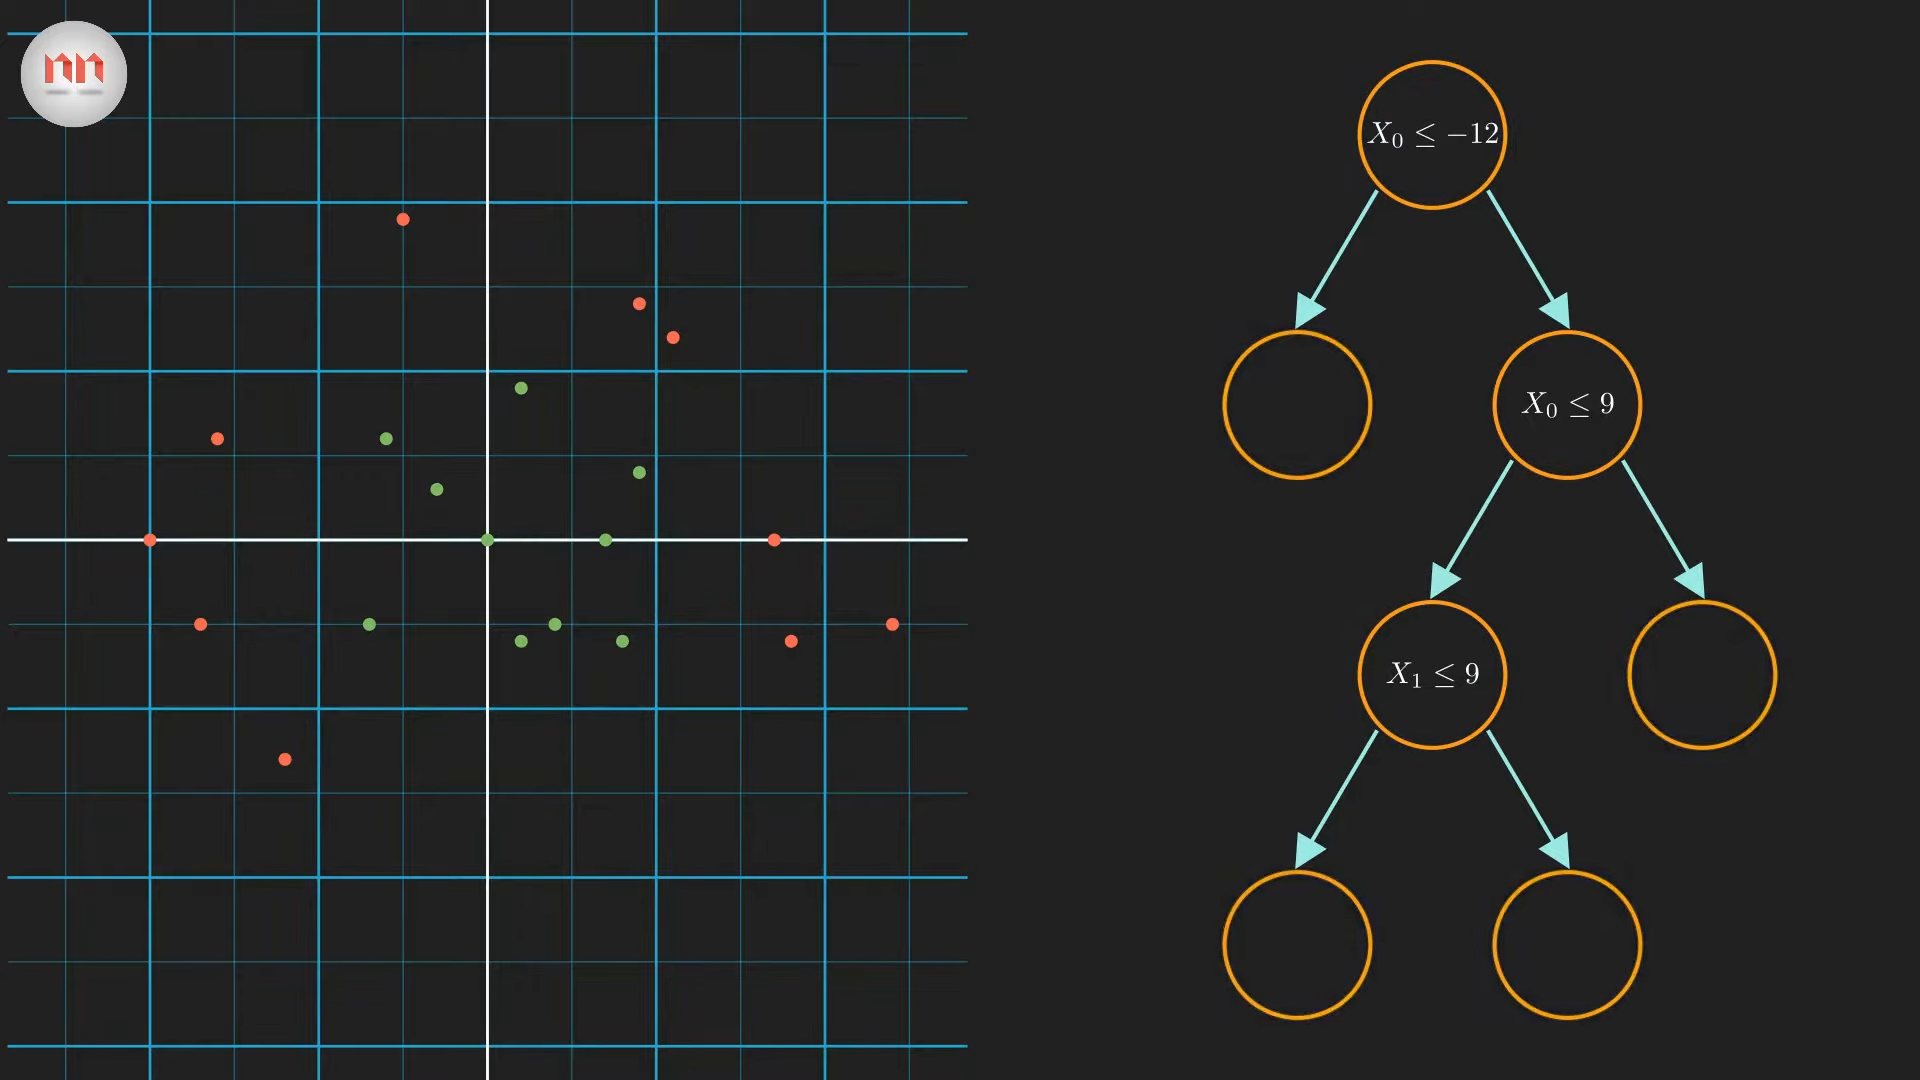
\includegraphics[width=13cm]{dt/_1-40 screenshot}
{\tiny \href{https://www.youtube.com/watch?v=ZVR2Way4nwQ}{ \copyright Normalized Nerd}}
\end{frame}

\begin{frame}{First split of points by x0}
\hspace*{-1cm}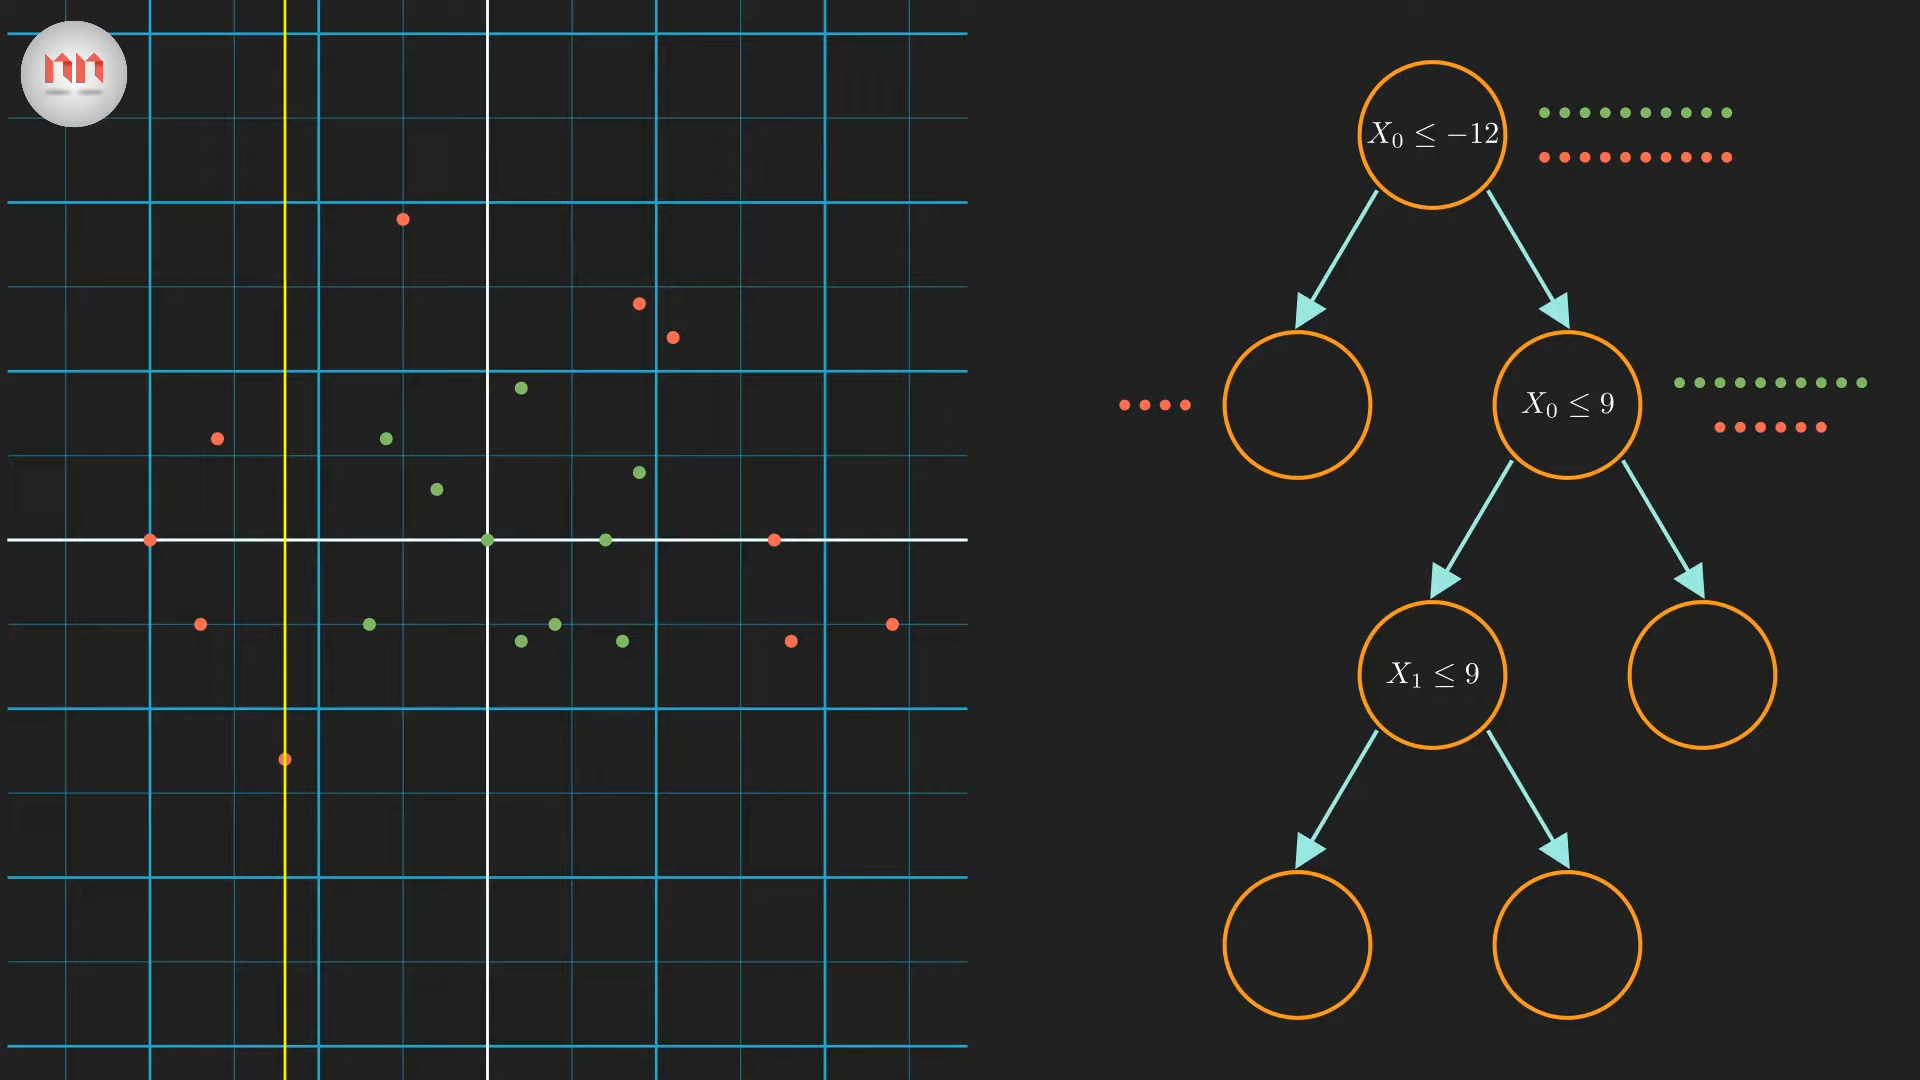
\includegraphics[width=13cm]{dt/_2-33 screenshot}
{\tiny \href{https://www.youtube.com/watch?v=ZVR2Way4nwQ}{ \copyright Normalized Nerd}}
\end{frame}

\begin{frame}{Second split of points by x0}
\hspace*{-1cm}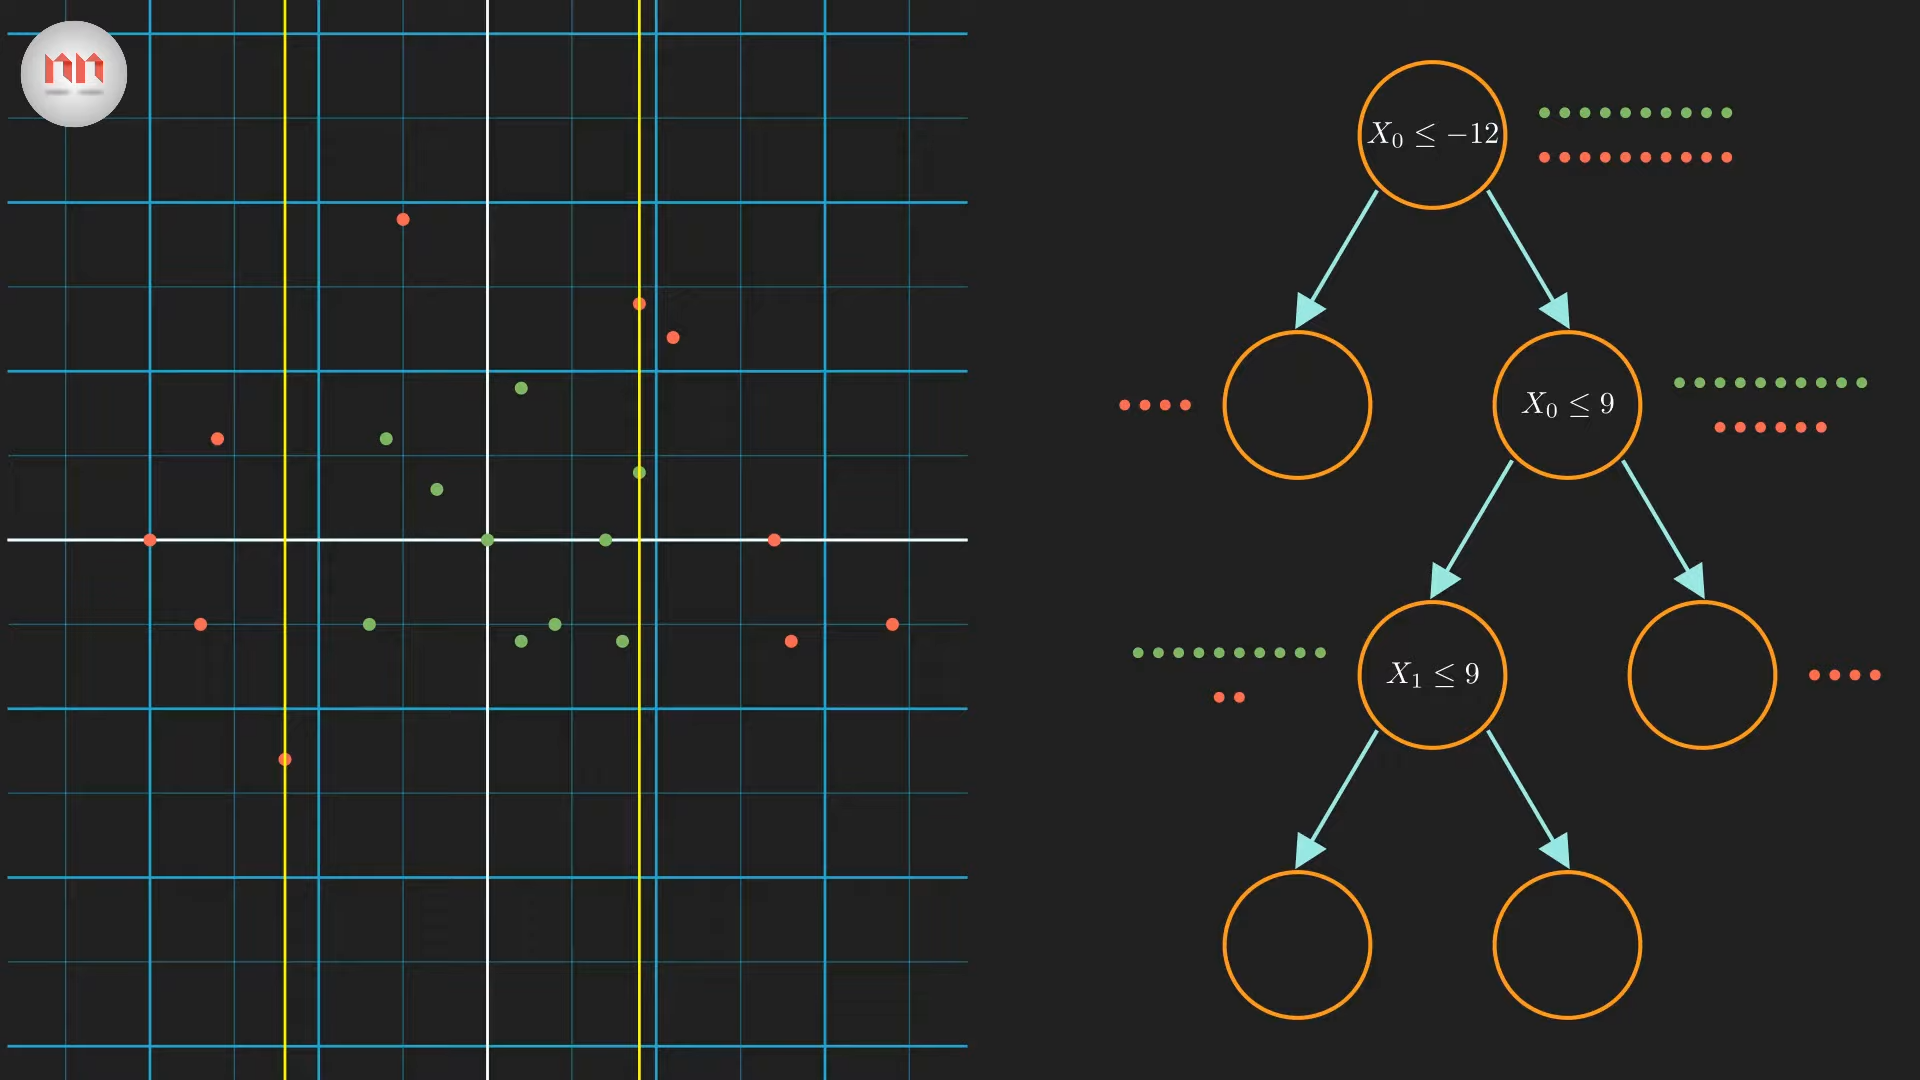
\includegraphics[width=13cm]{dt/_3-3 screenshot}
{\tiny \href{https://www.youtube.com/watch?v=ZVR2Way4nwQ}{ \copyright Normalized Nerd}}
\end{frame}

\begin{frame}{Third split of points by x1}
\hspace*{-1cm}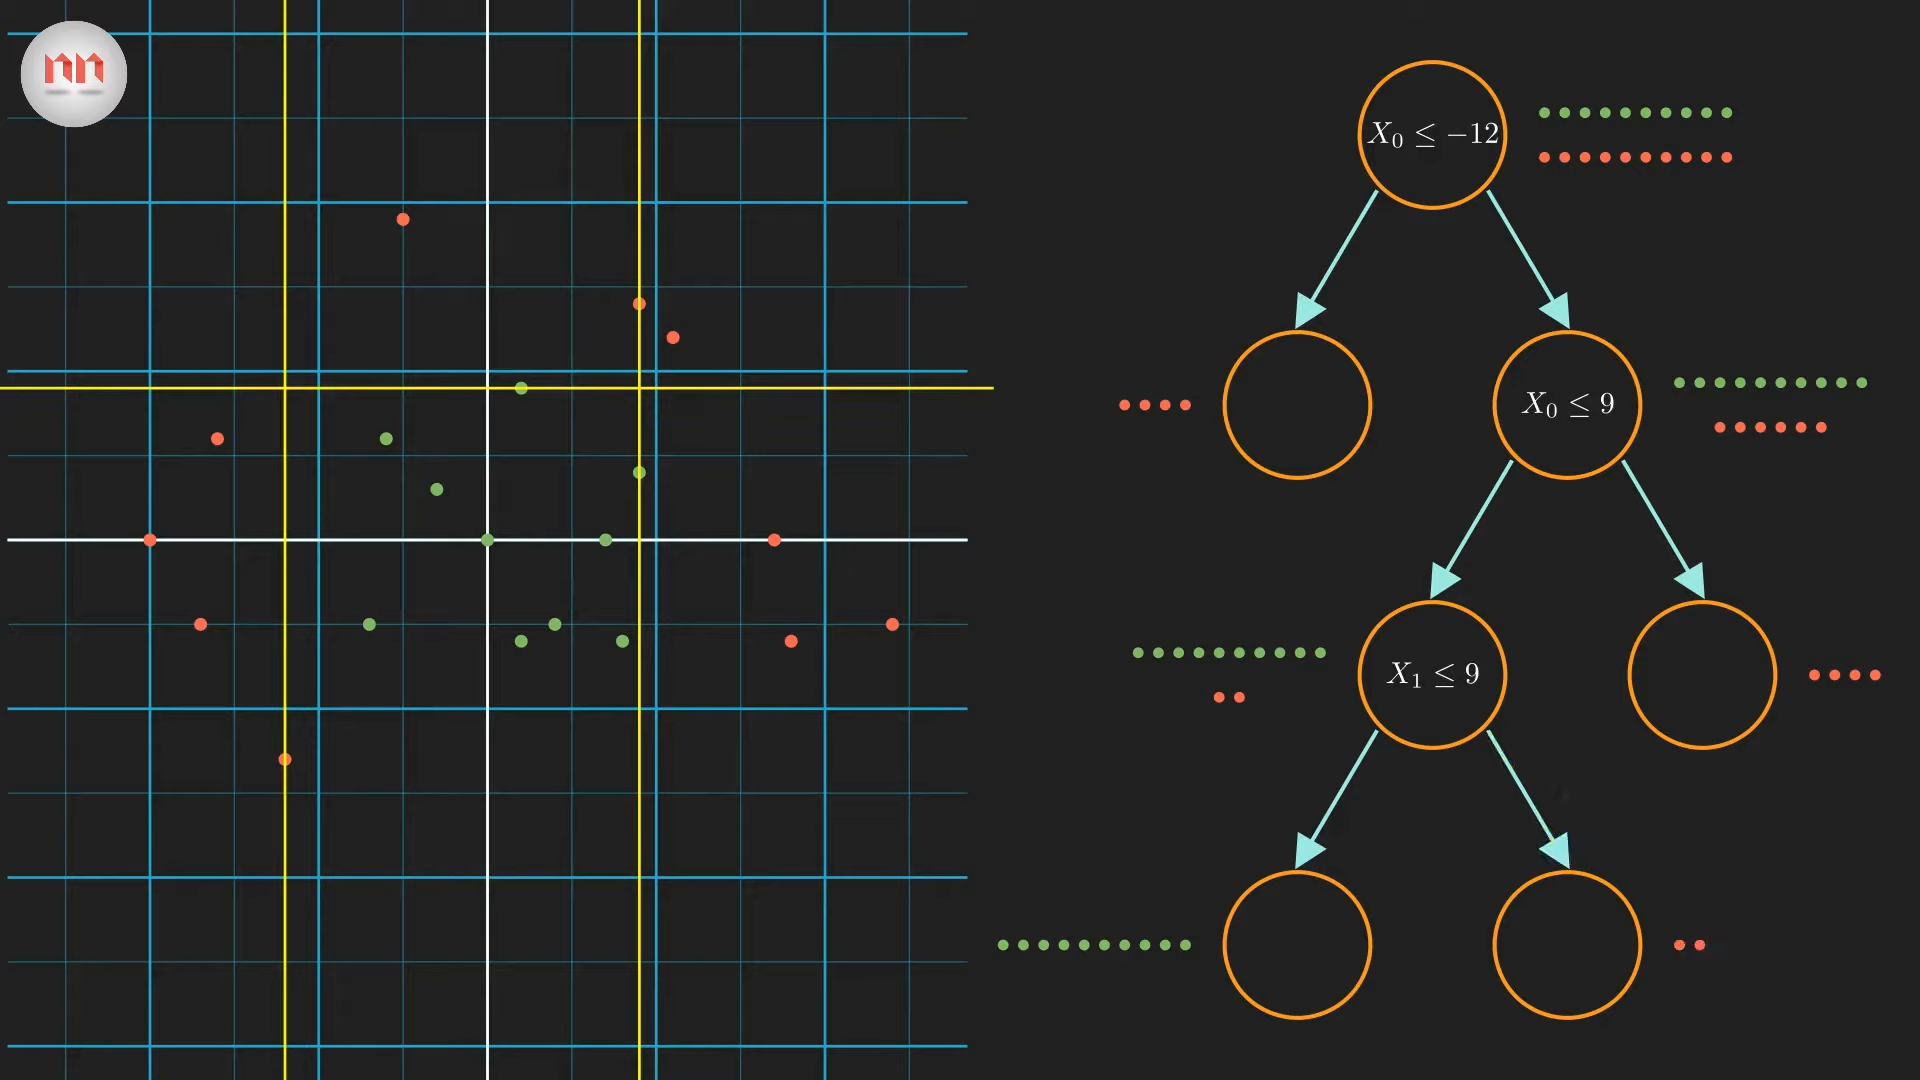
\includegraphics[width=13cm]{dt/_3-19 screenshot}
{\tiny \href{https://www.youtube.com/watch?v=ZVR2Way4nwQ}{ \copyright Normalized Nerd}}
\end{frame}

\begin{frame}{How to use the decision tree to classify point (15,7)}
\hspace*{-1cm}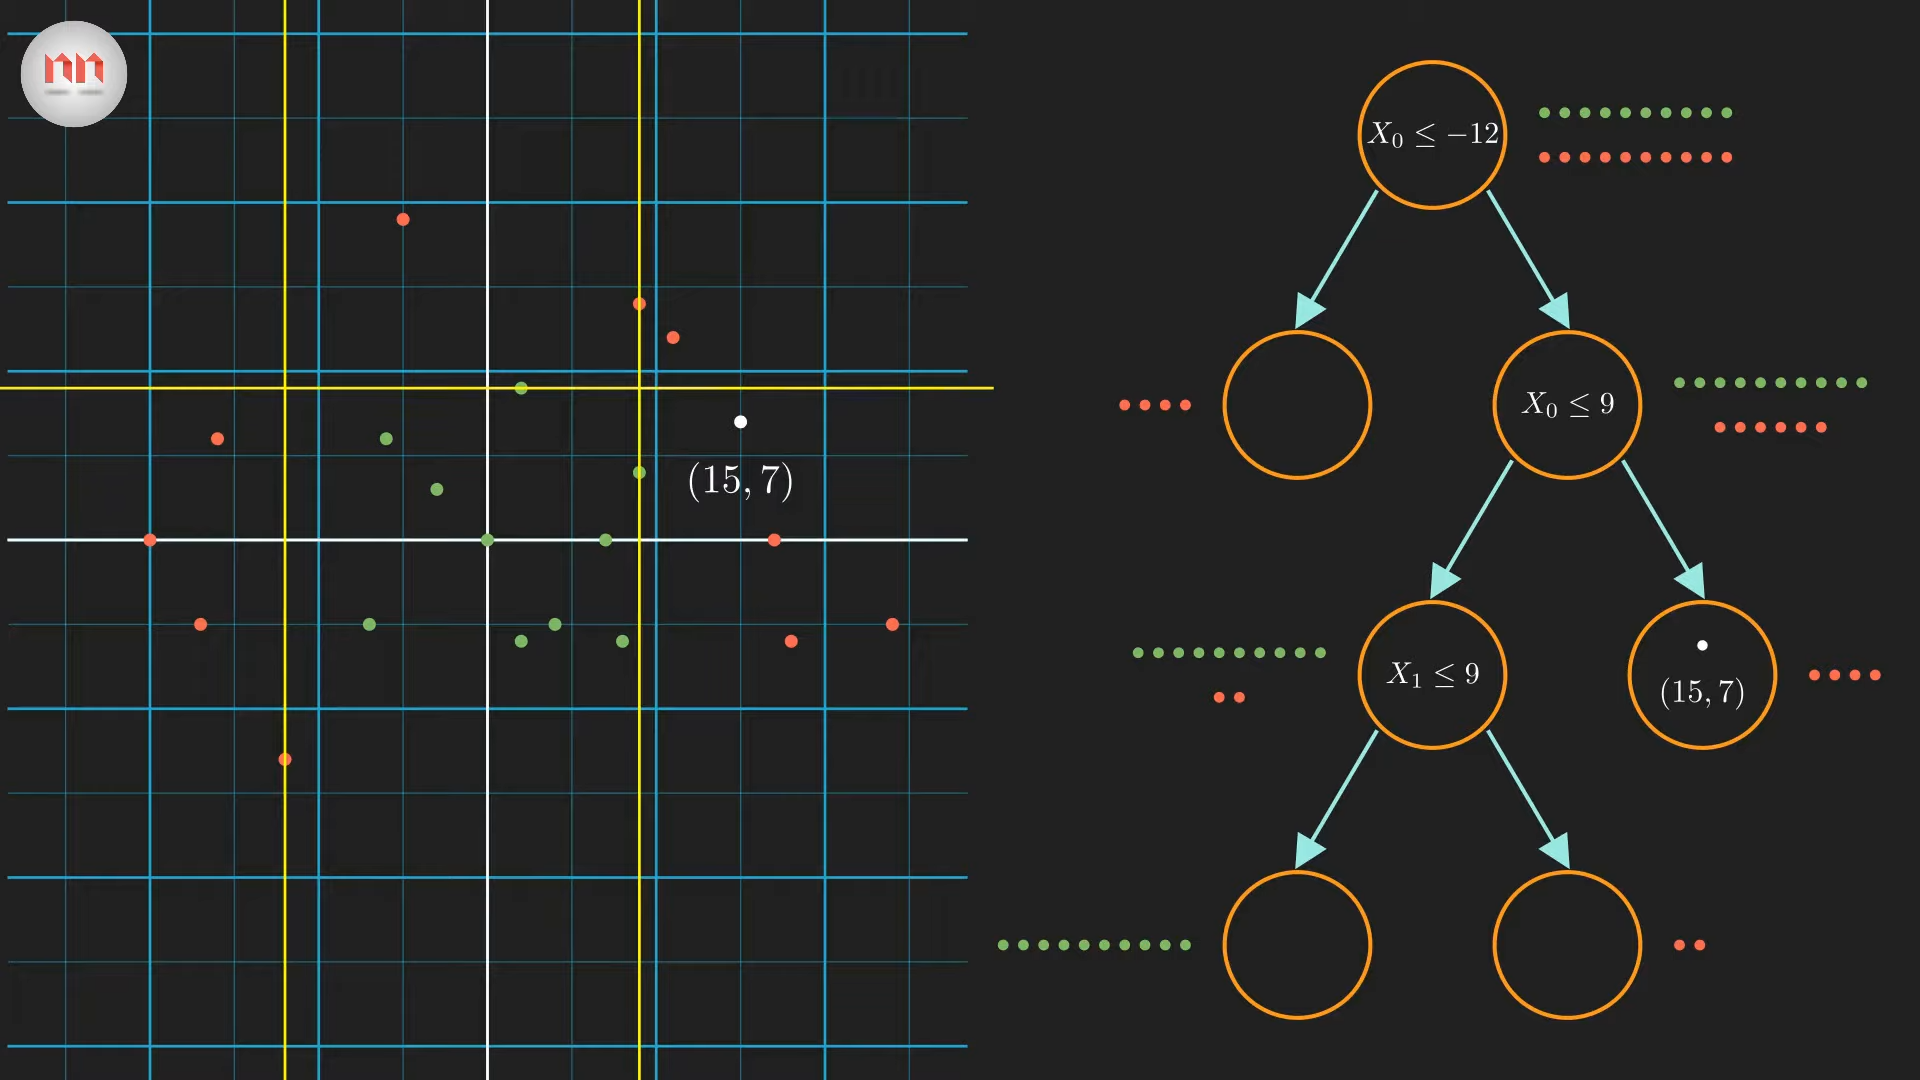
\includegraphics[width=13cm]{dt/_3-54 screenshot}
{\tiny \href{https://www.youtube.com/watch?v=ZVR2Way4nwQ}{ \copyright Normalized Nerd}}
\end{frame}

\begin{frame}{Classification space}
\hspace*{-1cm}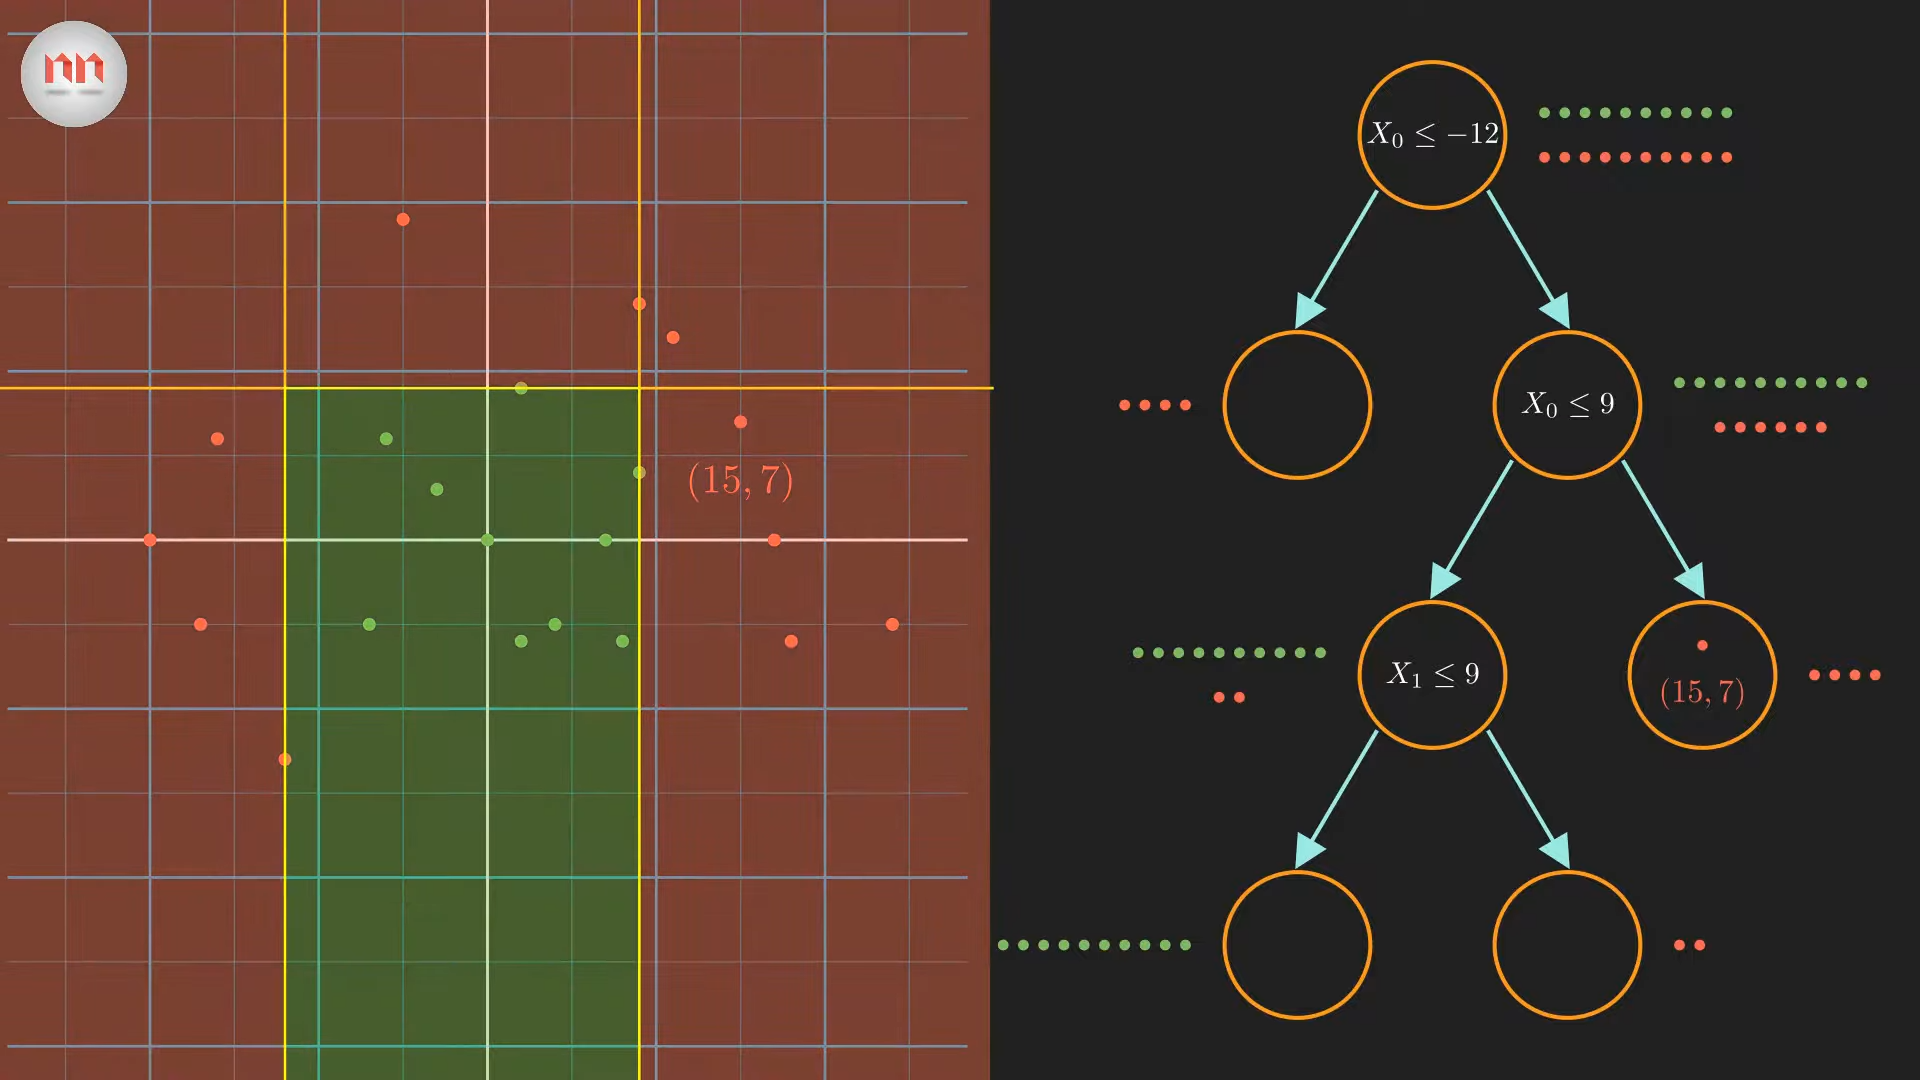
\includegraphics[width=13cm]{dt/_4-22 screenshot}
{\tiny \href{https://www.youtube.com/watch?v=ZVR2Way4nwQ}{ \copyright Normalized Nerd}}
\end{frame}

\begin{frame}{Building tree: how to split}
\hspace*{-1cm}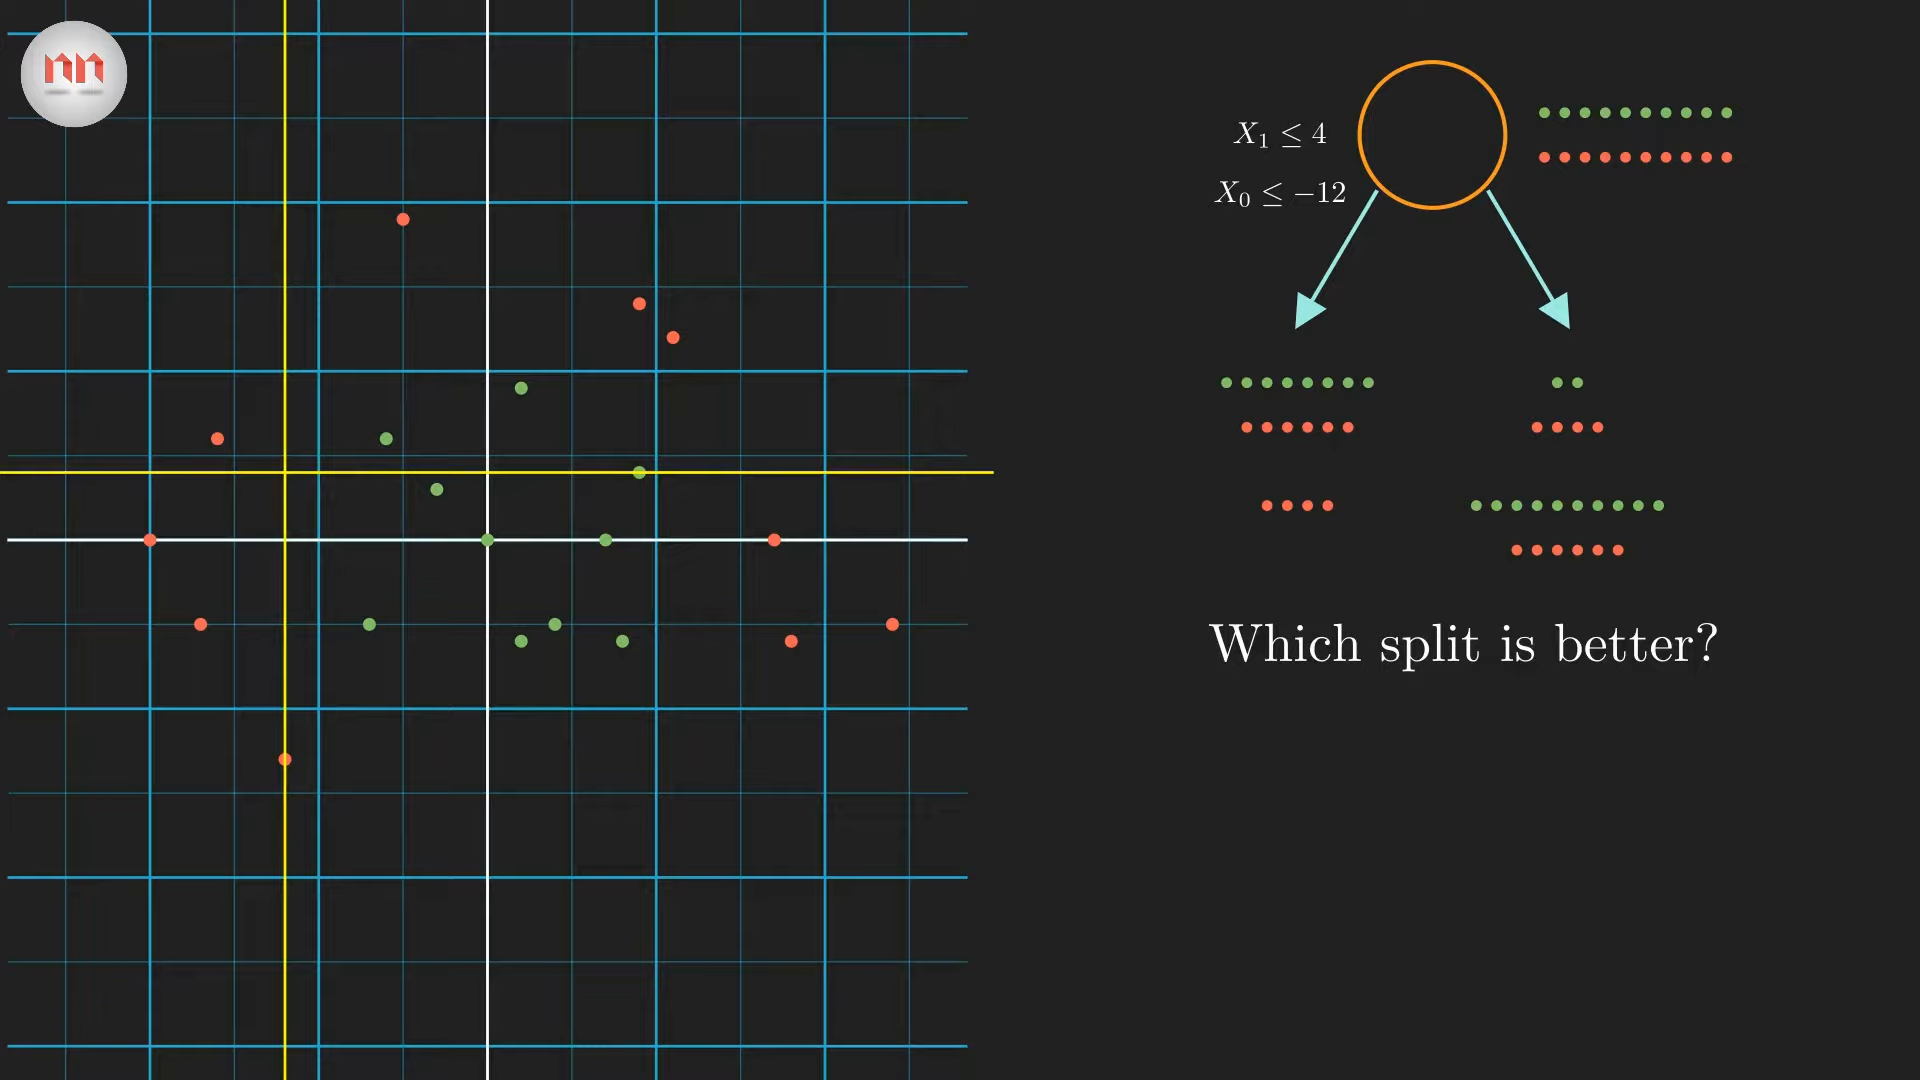
\includegraphics[width=13cm]{dt/_5-55 screenshot}
{\tiny \href{https://www.youtube.com/watch?v=ZVR2Way4nwQ}{ \copyright Normalized Nerd}}
\end{frame}

\begin{frame}{Building tree: entropy - measure of informativeness}
\hspace*{-1cm}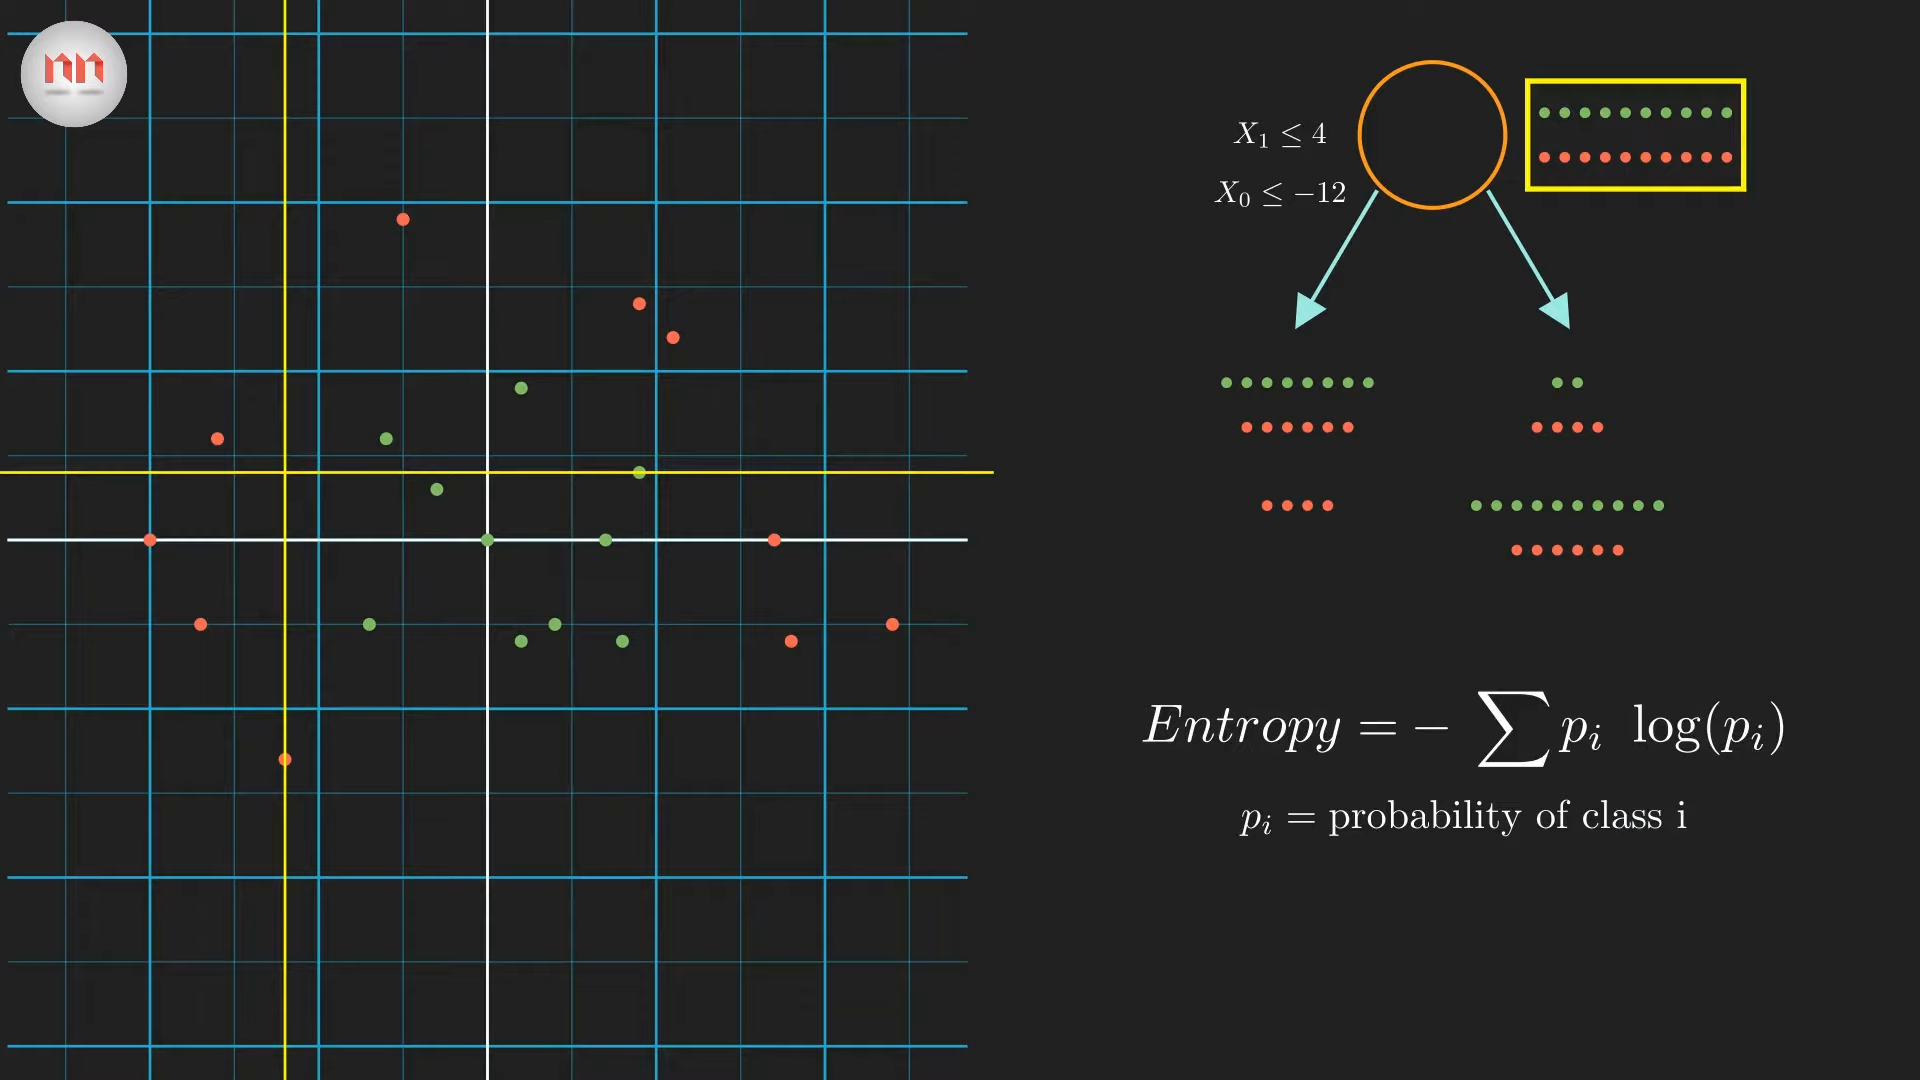
\includegraphics[width=13cm]{dt/_7-2 screenshot}
{\tiny \href{https://www.youtube.com/watch?v=ZVR2Way4nwQ}{ \copyright Normalized Nerd}}
\end{frame}

\begin{frame}{Building tree: entropy - measure of informativeness}
\hspace*{-1cm}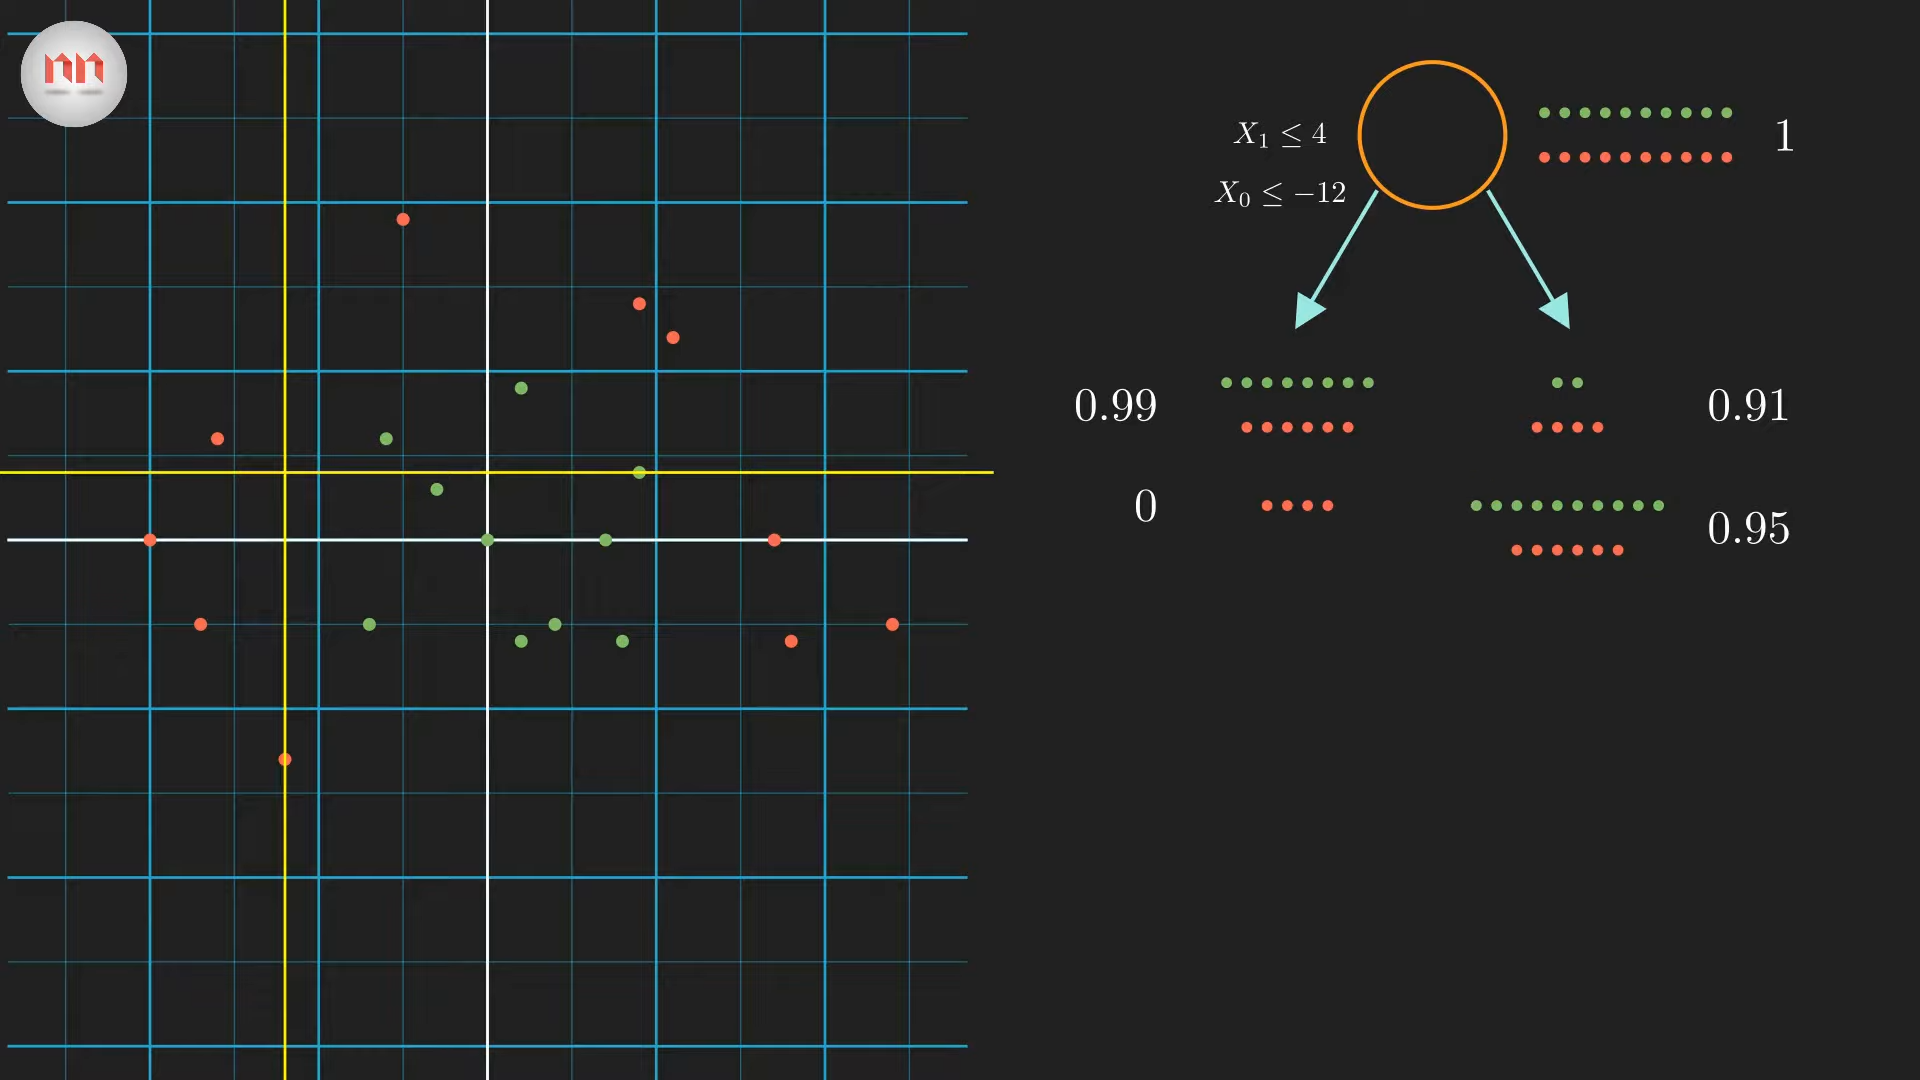
\includegraphics[width=13cm]{dt/_7-52 screenshot}
{\tiny \href{https://www.youtube.com/watch?v=ZVR2Way4nwQ}{ \copyright Normalized Nerd}}
\end{frame}

\begin{frame}{Building tree: information gain (IG)}
\hspace*{-1cm}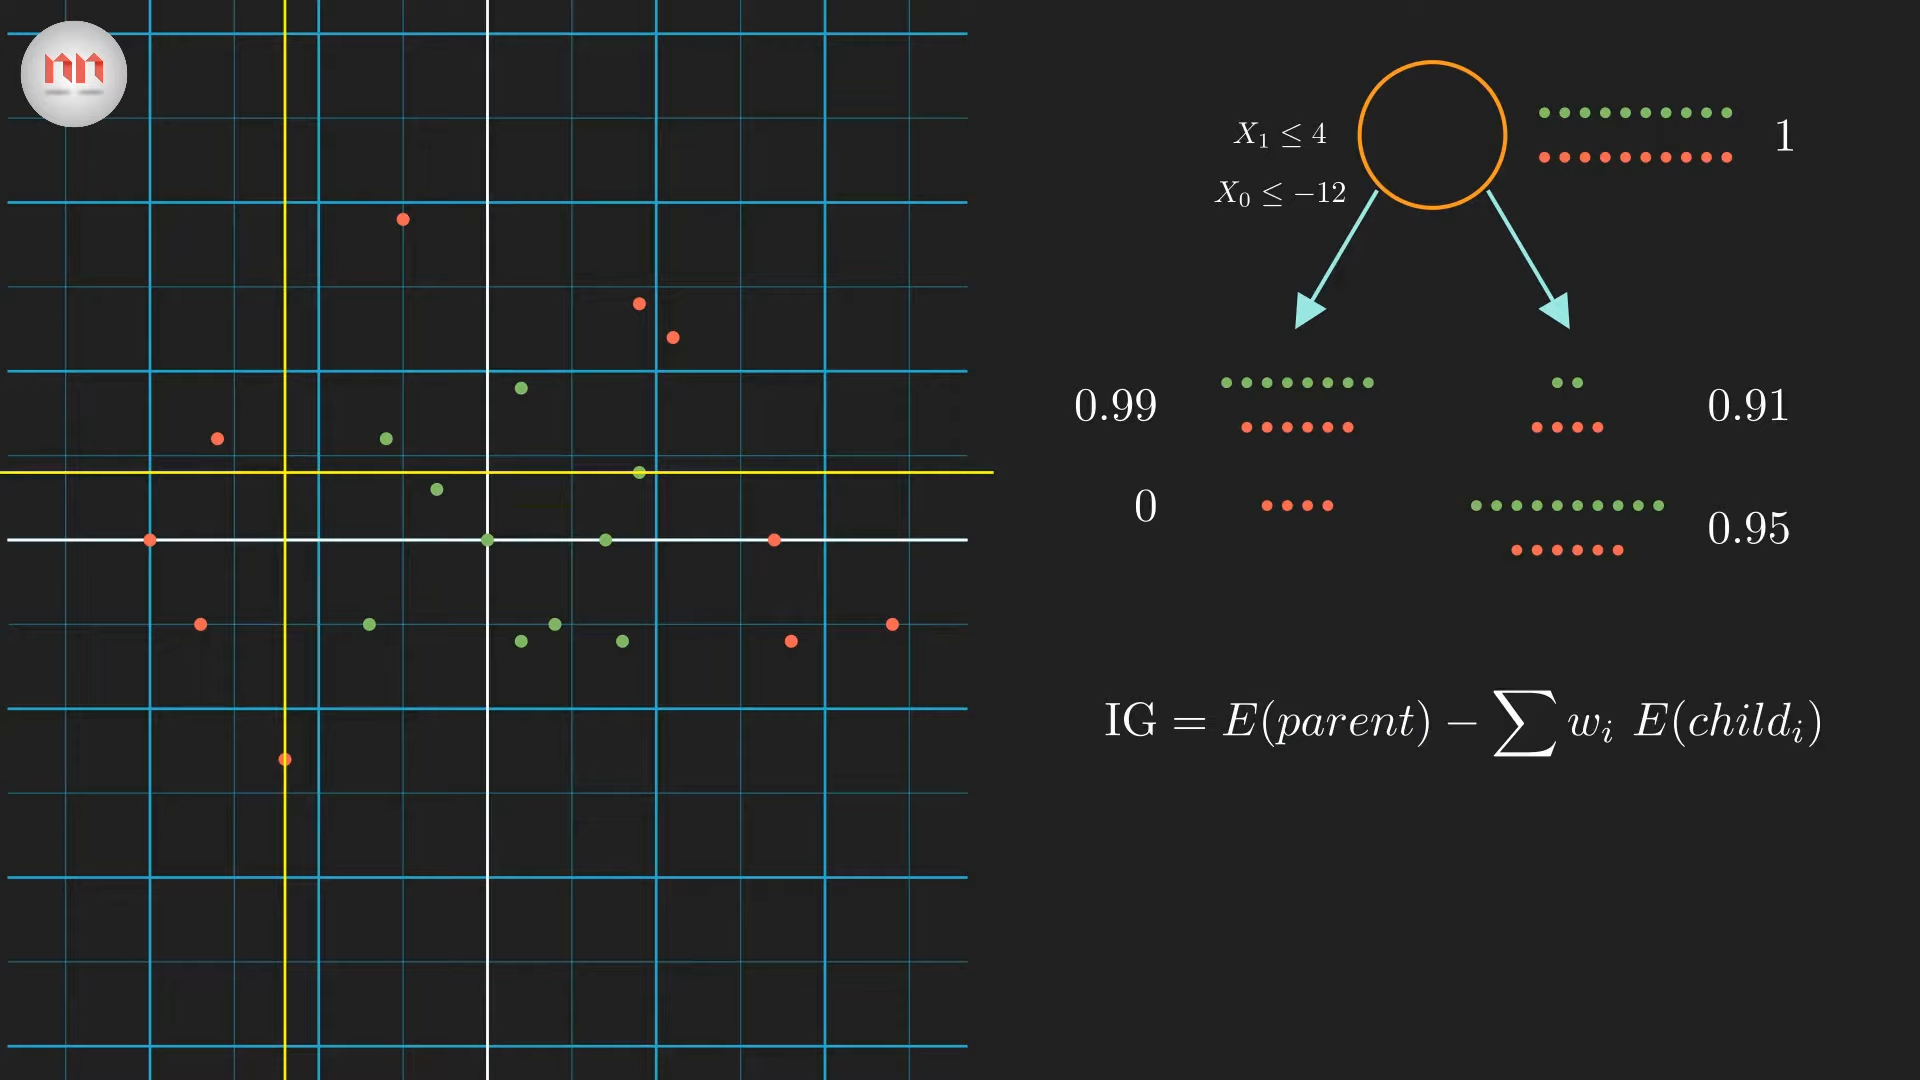
\includegraphics[width=13cm]{dt/_8-11 screenshot}
{\tiny \href{https://www.youtube.com/watch?v=ZVR2Way4nwQ}{ \copyright Normalized Nerd}}
\end{frame}

\begin{frame}{Building tree: information gain (IG)}
\hspace*{-1cm}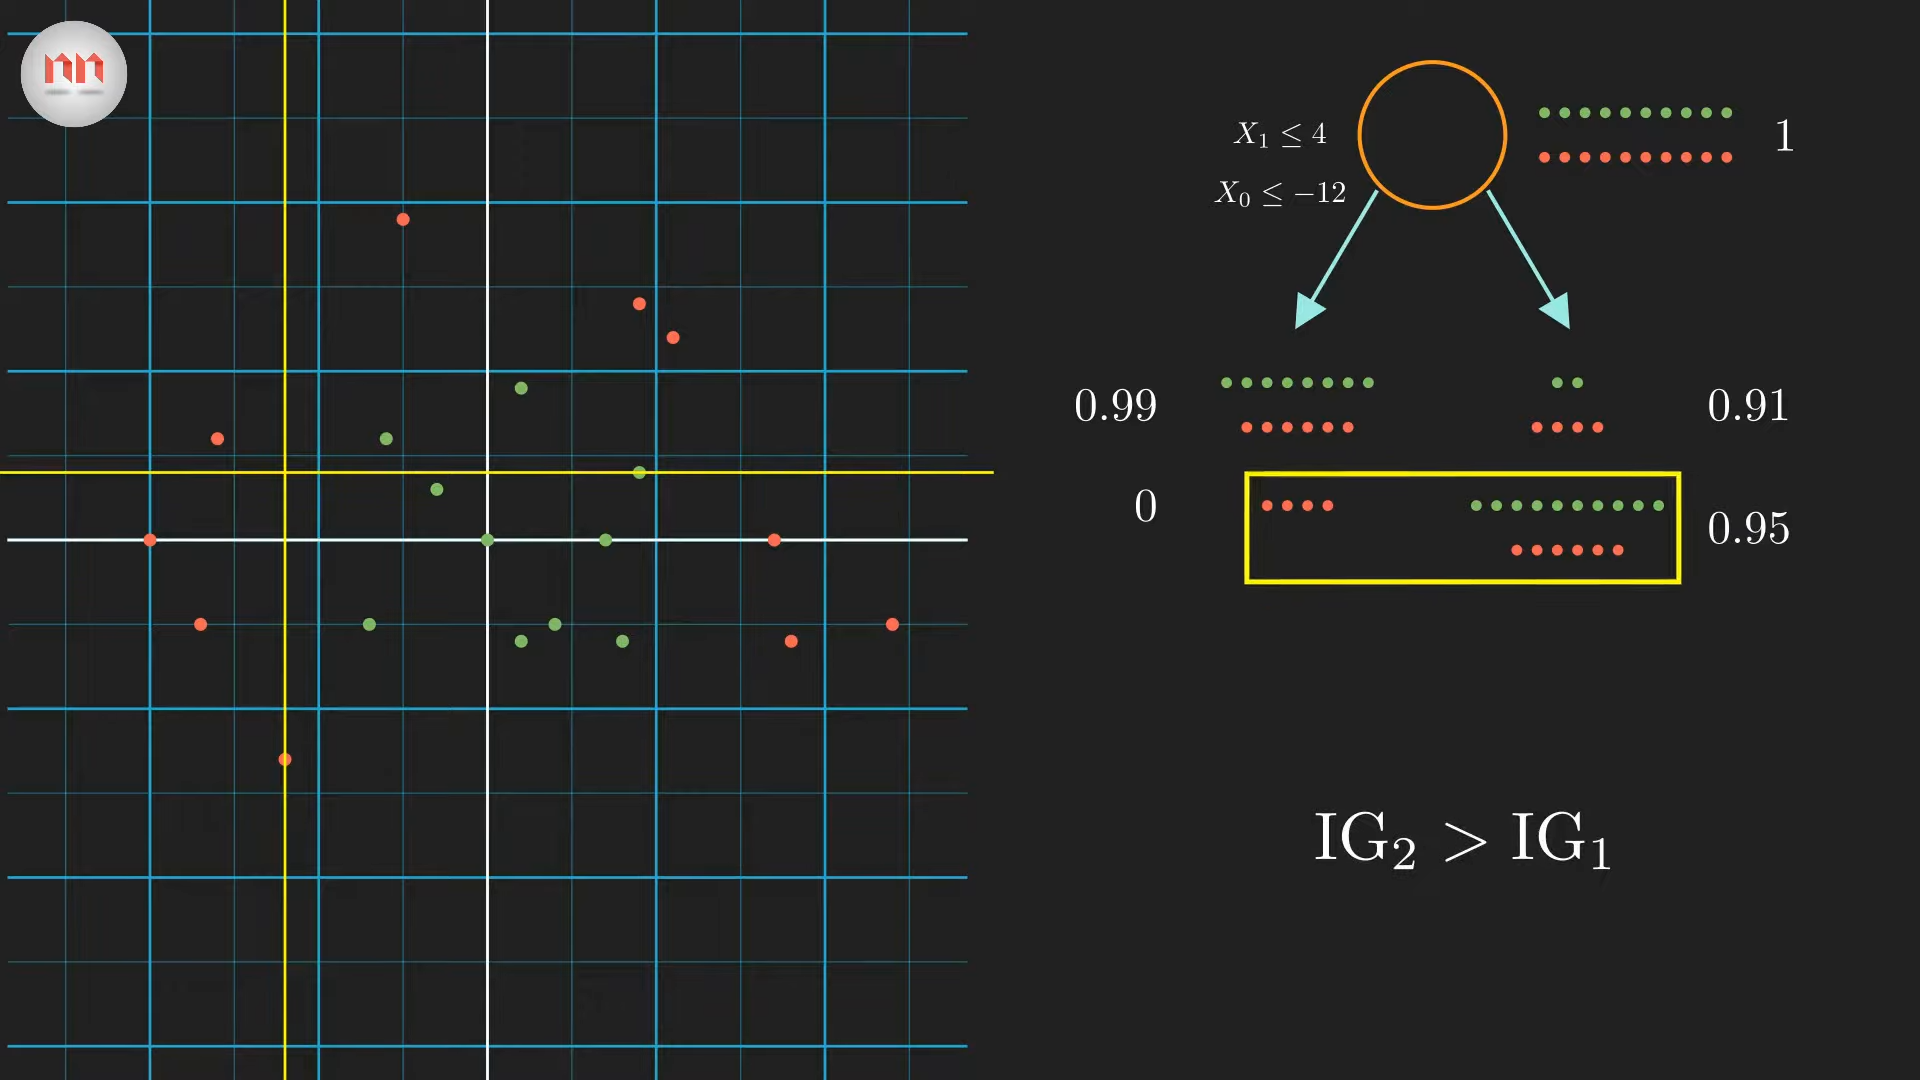
\includegraphics[width=13cm]{dt/_8-32 screenshot}
{\tiny \href{https://www.youtube.com/watch?v=ZVR2Way4nwQ}{ \copyright Normalized Nerd}}
\end{frame}

%\fi

\begin{frame}{Summary: decision tree algorithm}
\begin{block}{Build a decision tree}
\begin{itemize}
    \item Loop over all points
    \begin{itemize}
        \item Split the dataset by the point position
        \item Compute entropy for left and right sub-datasets
        \item Compute information gain (IG)
    \end{itemize}
    \item Use the highest IG and create a decision node
    \item Split the dataset into left and right sub-dataset
    \item Recursively build the tree for the left and right sub-datasets
\end{itemize}
\end{block}
\end{frame}

\section{Random forest}

%\iffalse

\begin{frame}{Dataset: 6 points, 5 features, 2 classes}
\hspace*{-1cm}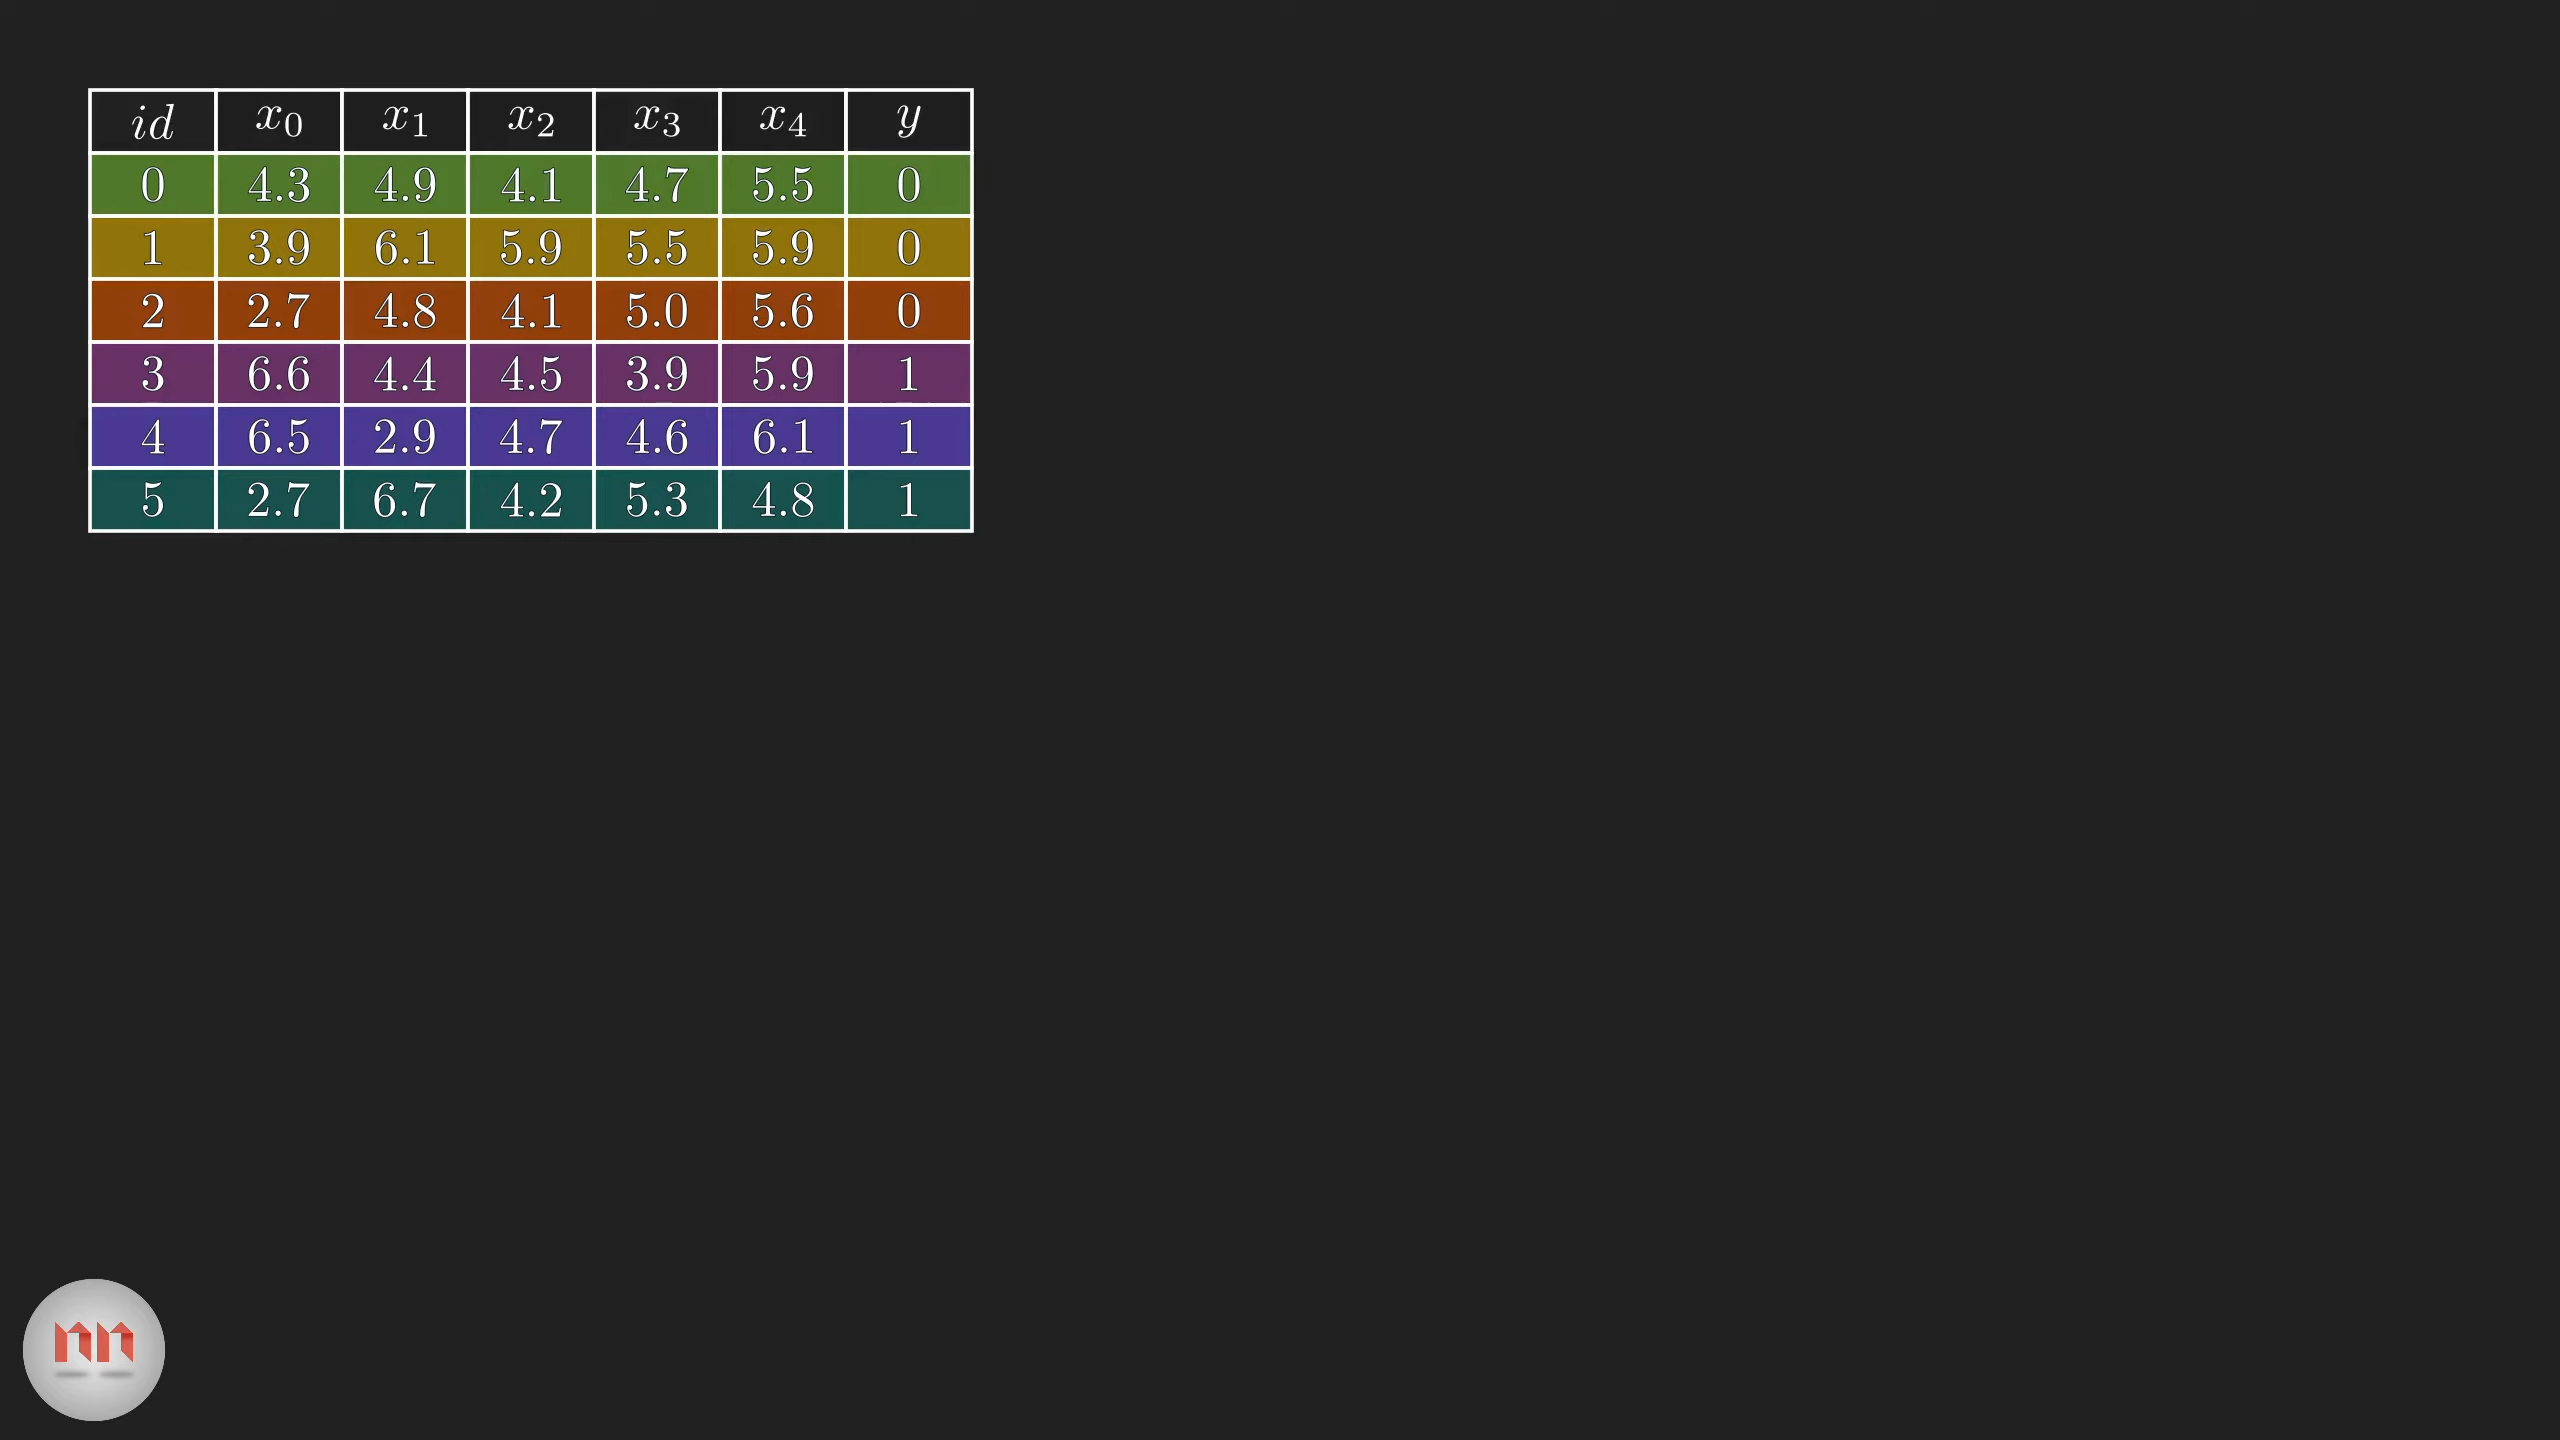
\includegraphics[width=13cm]{figs/rf/_0-40 screenshot.png}
{\tiny \href{https://www.youtube.com/watch?v=ZVR2Way4nwQ}{ \copyright Normalized Nerd}}
\end{frame}

\begin{frame}{A simple working decision tree}
\hspace*{-1cm}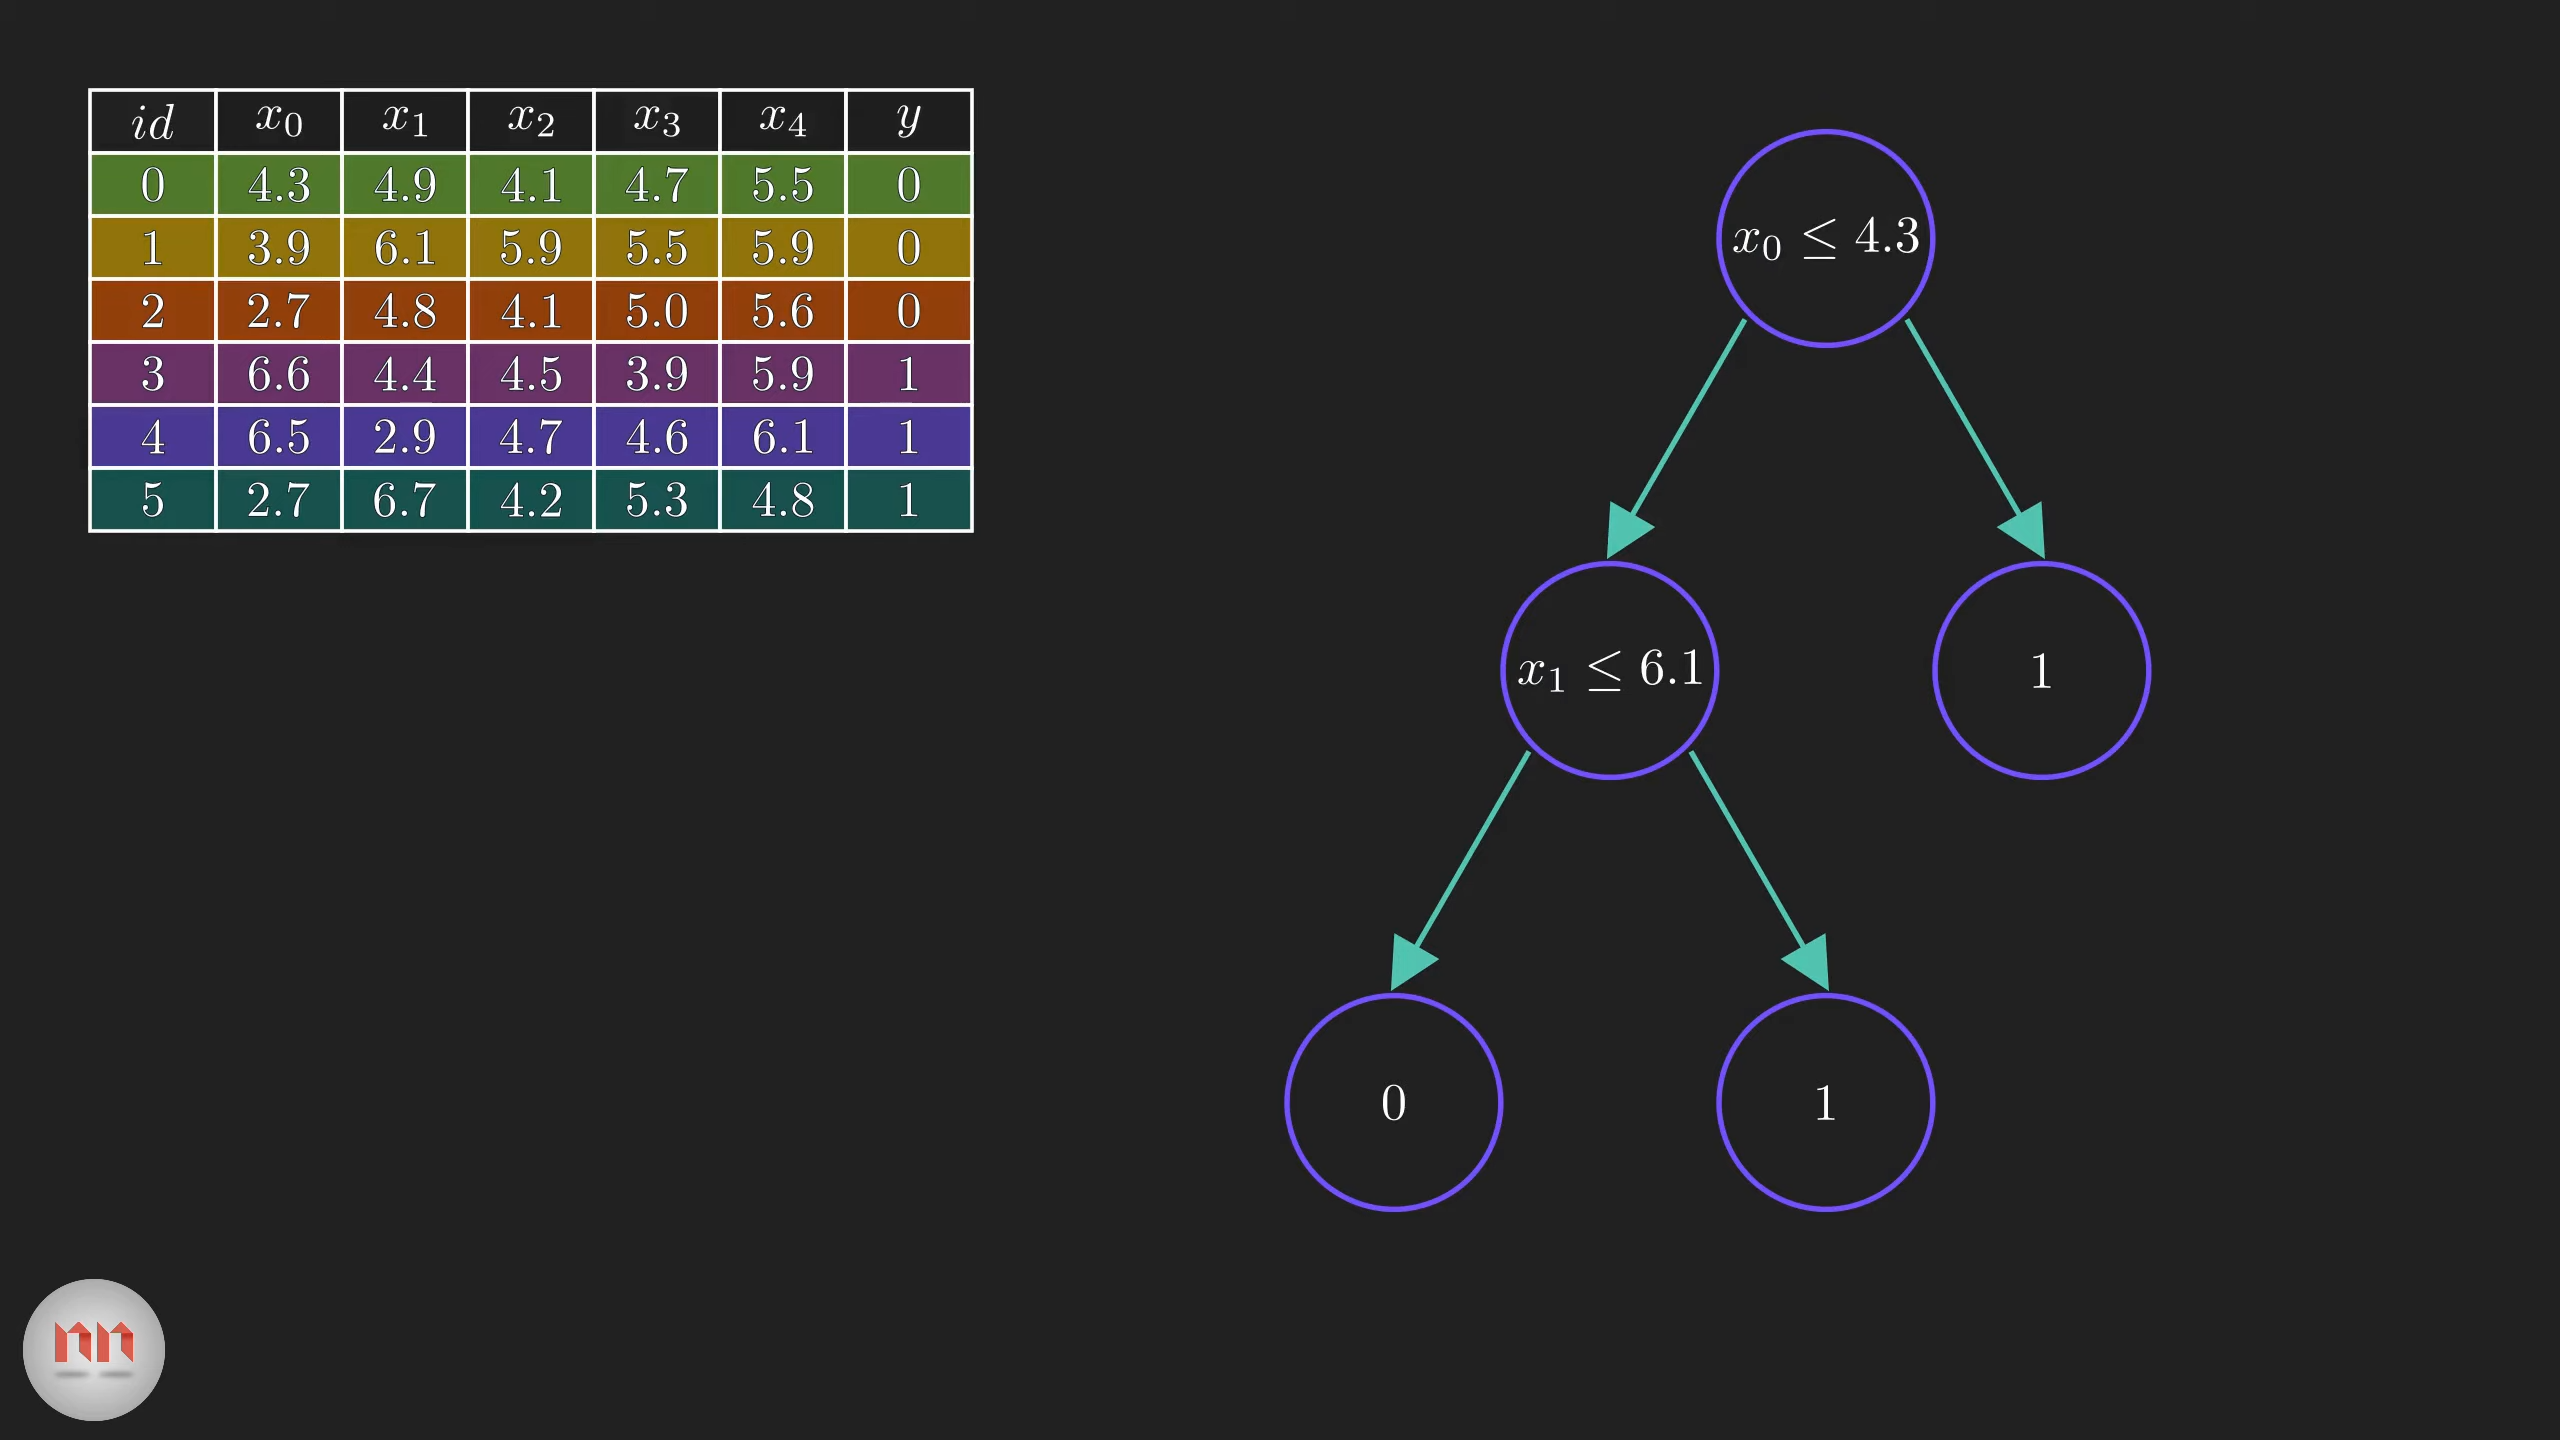
\includegraphics[width=13cm]{figs/rf/_1-6 screenshot.png}
{\tiny \href{https://www.youtube.com/watch?v=ZVR2Way4nwQ}{ \copyright Normalized Nerd}}
\end{frame}

\begin{frame}{What if values slightly change?}
\hspace*{-1cm}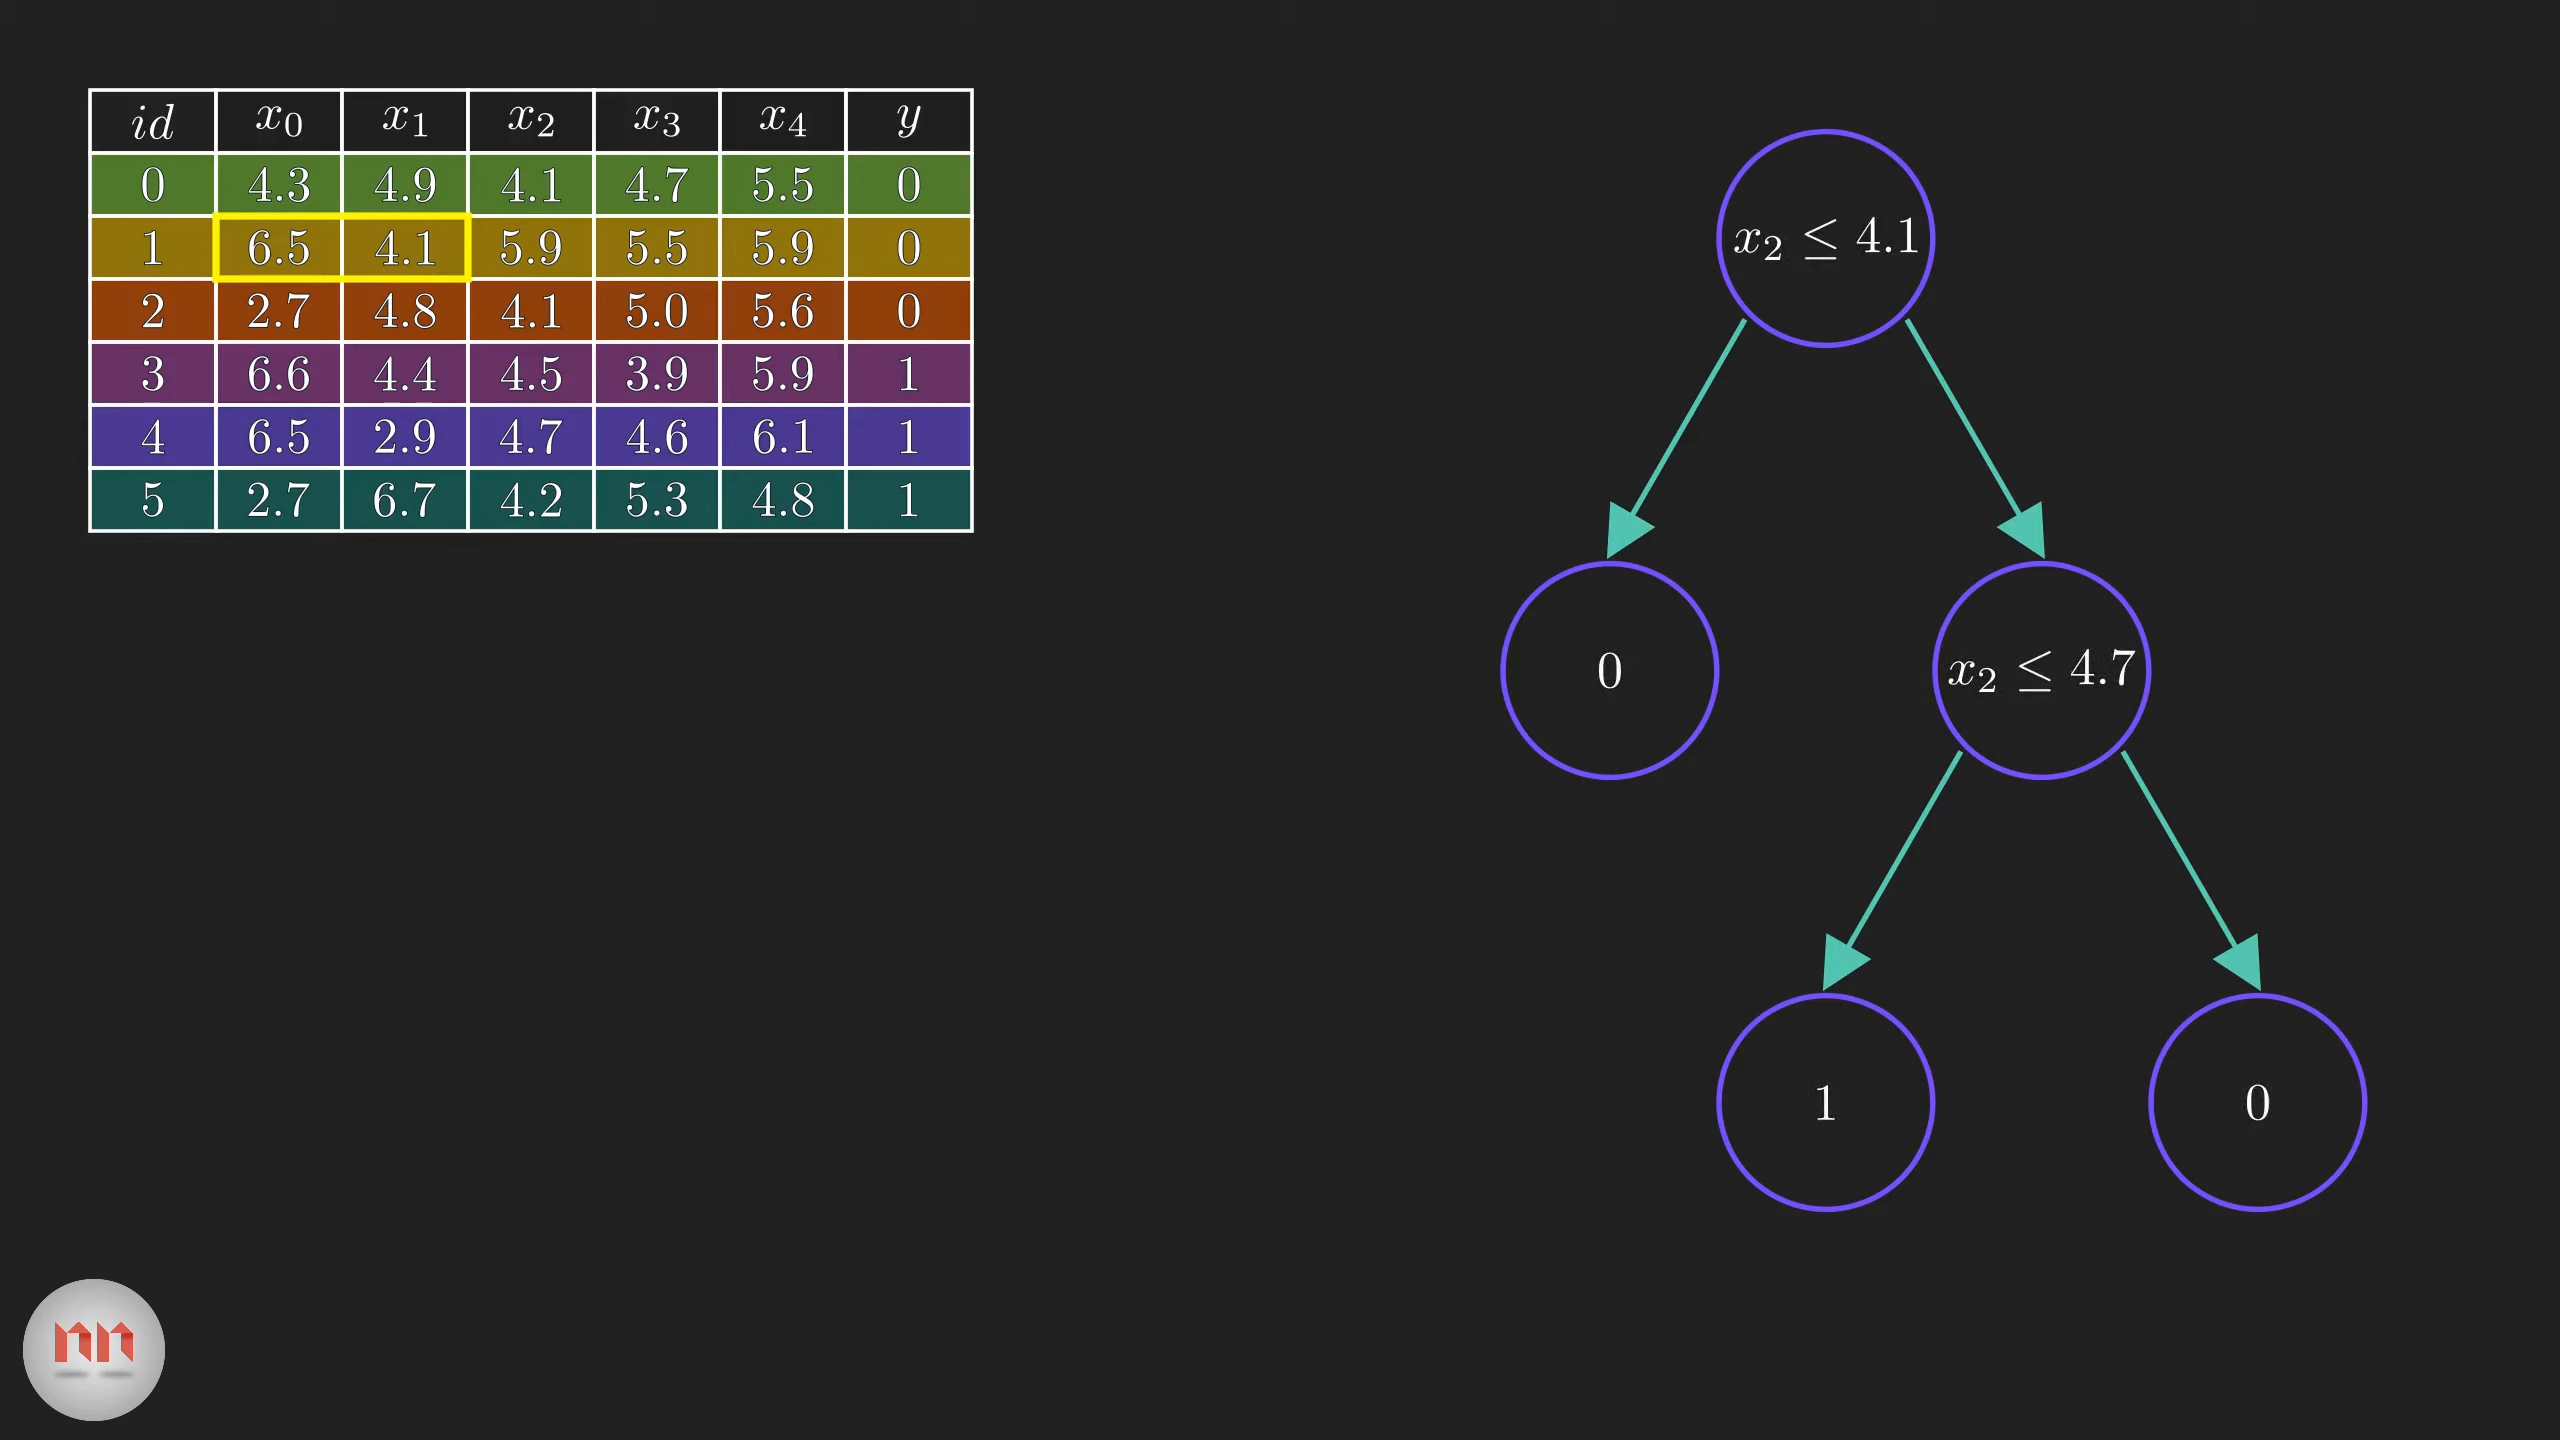
\includegraphics[width=13cm]{figs/rf/_2-6 screenshot.png}
{\tiny \href{https://www.youtube.com/watch?v=ZVR2Way4nwQ}{ \copyright Normalized Nerd}}
\end{frame}

\begin{frame}{4 random datasets: take 6 random point with repetition}
\hspace*{-1cm}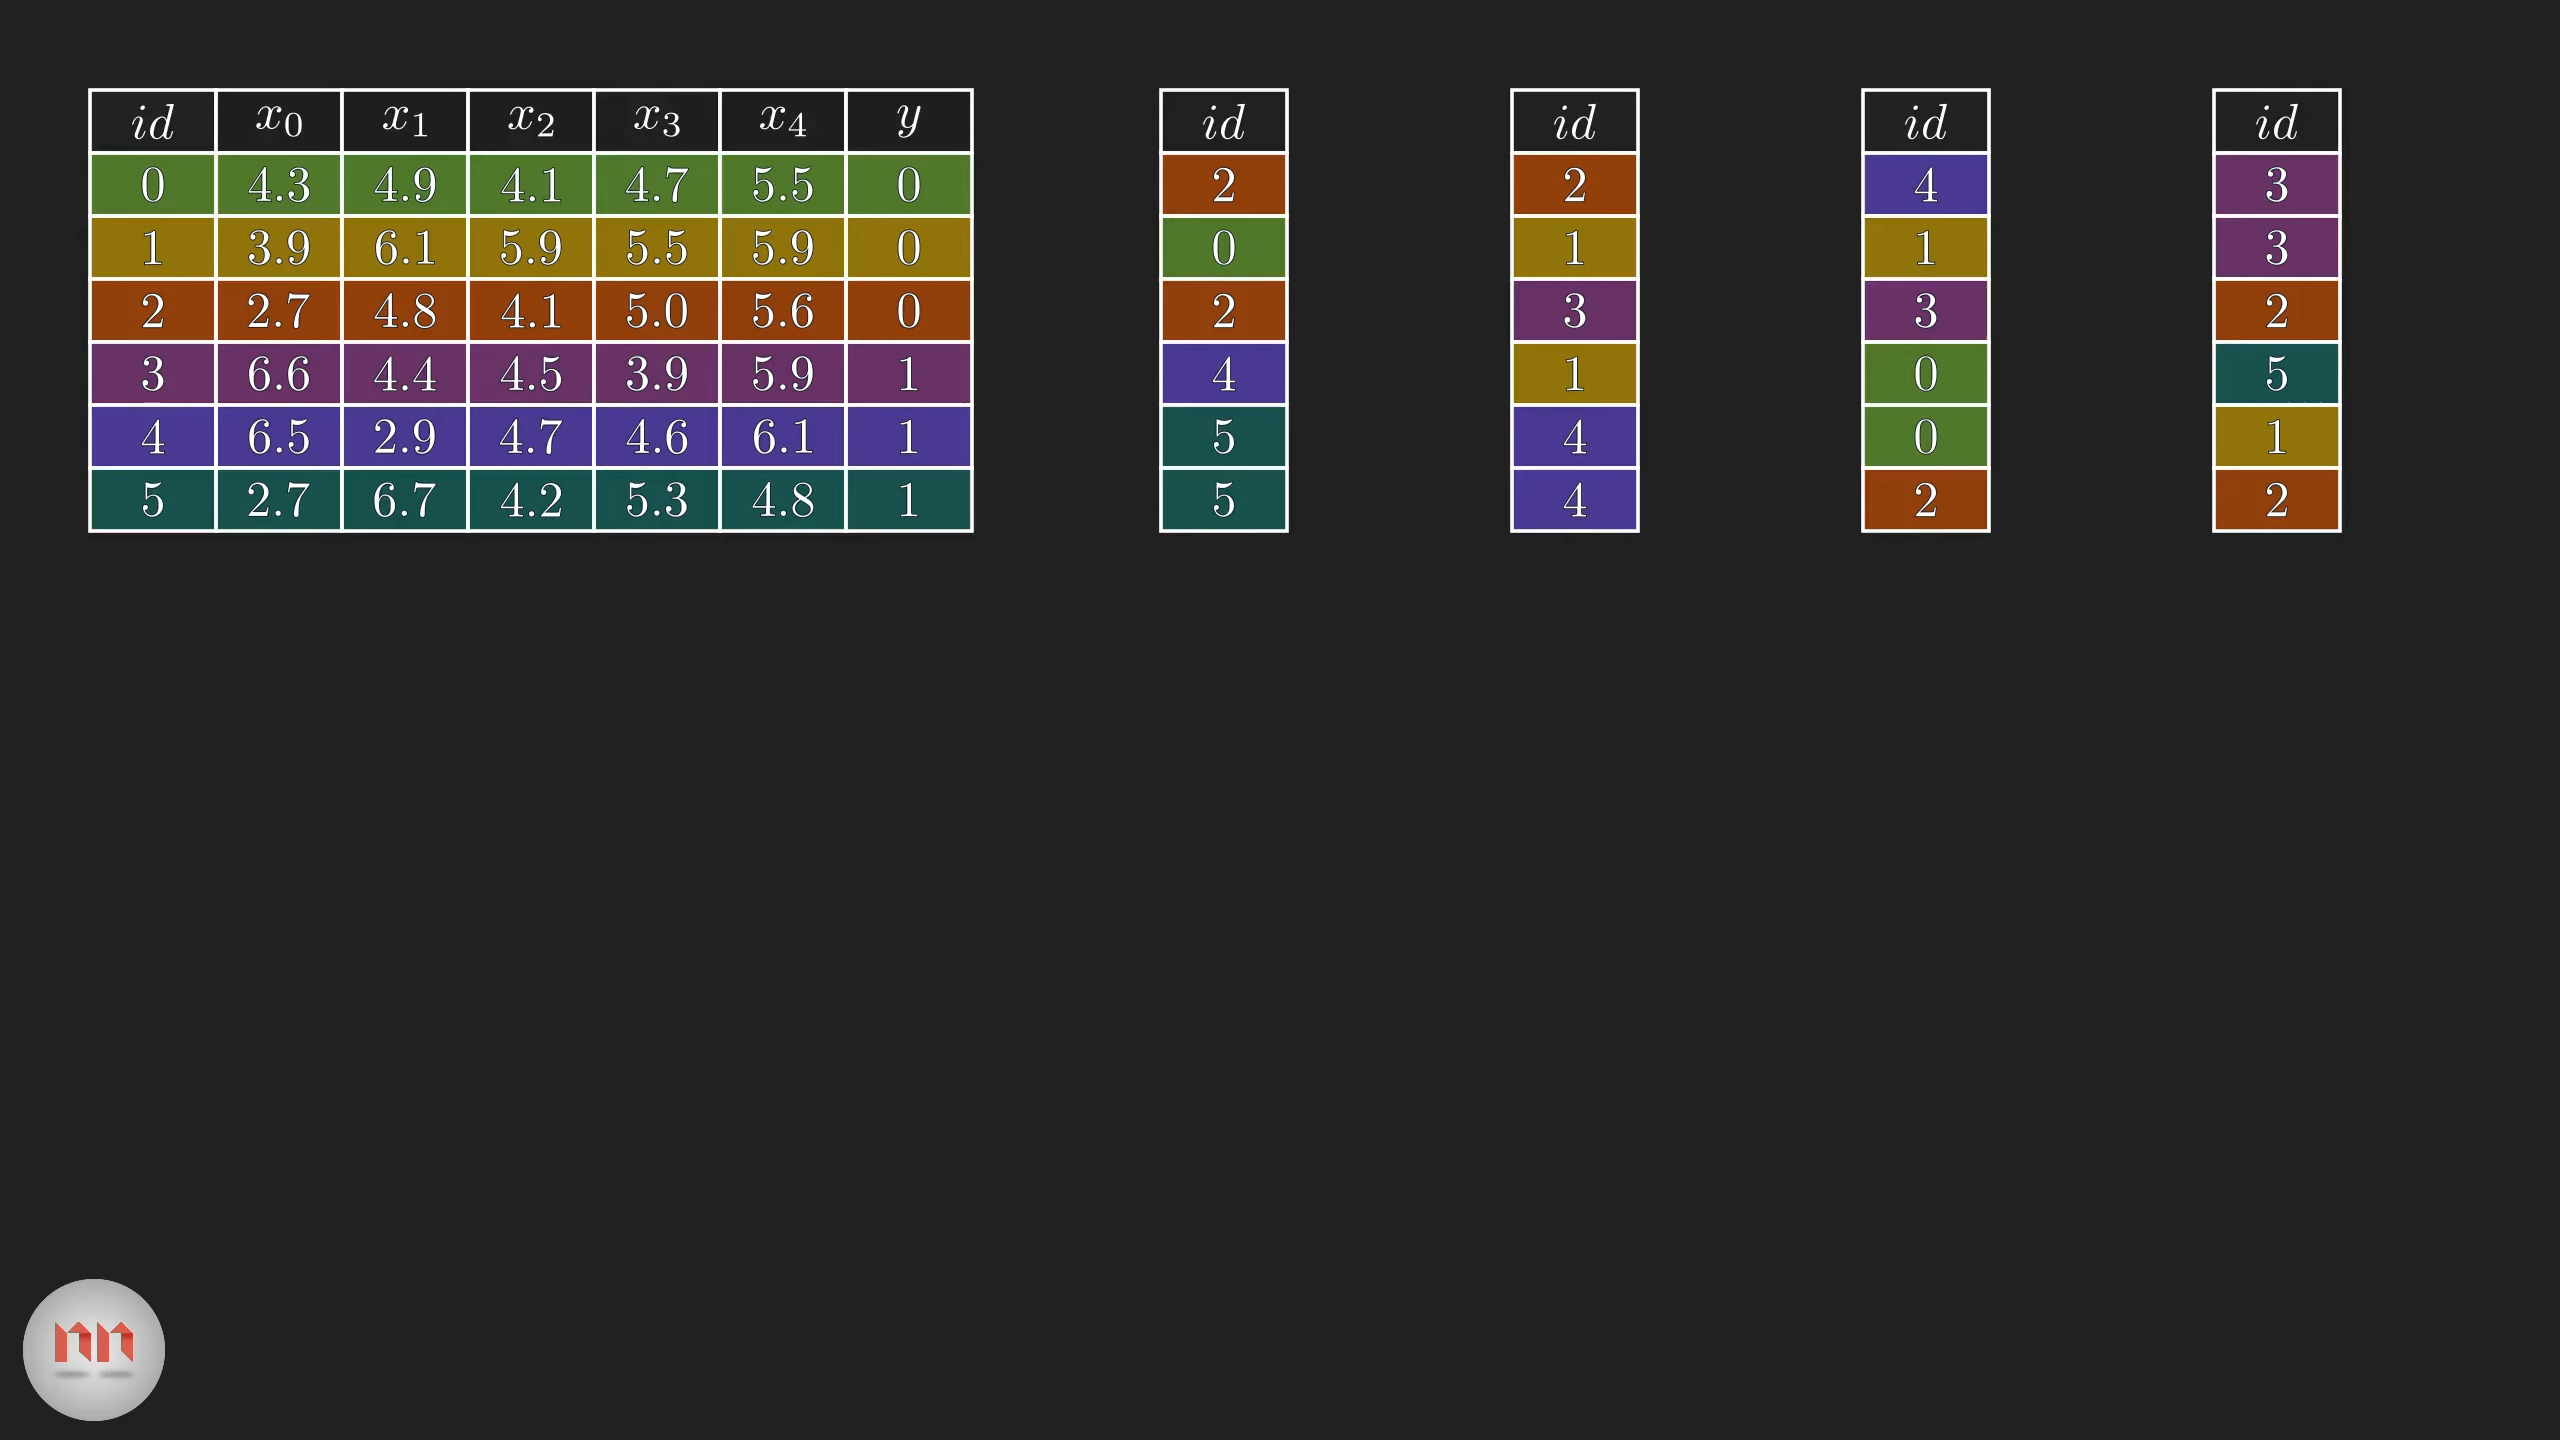
\includegraphics[width=13cm]{figs/rf/_3-33 screenshot.png}
{\tiny \href{https://www.youtube.com/watch?v=ZVR2Way4nwQ}{ \copyright Normalized Nerd}}
\end{frame}

\begin{frame}{Random sampling with repetition = Bootstrapping}
\hspace*{-1cm}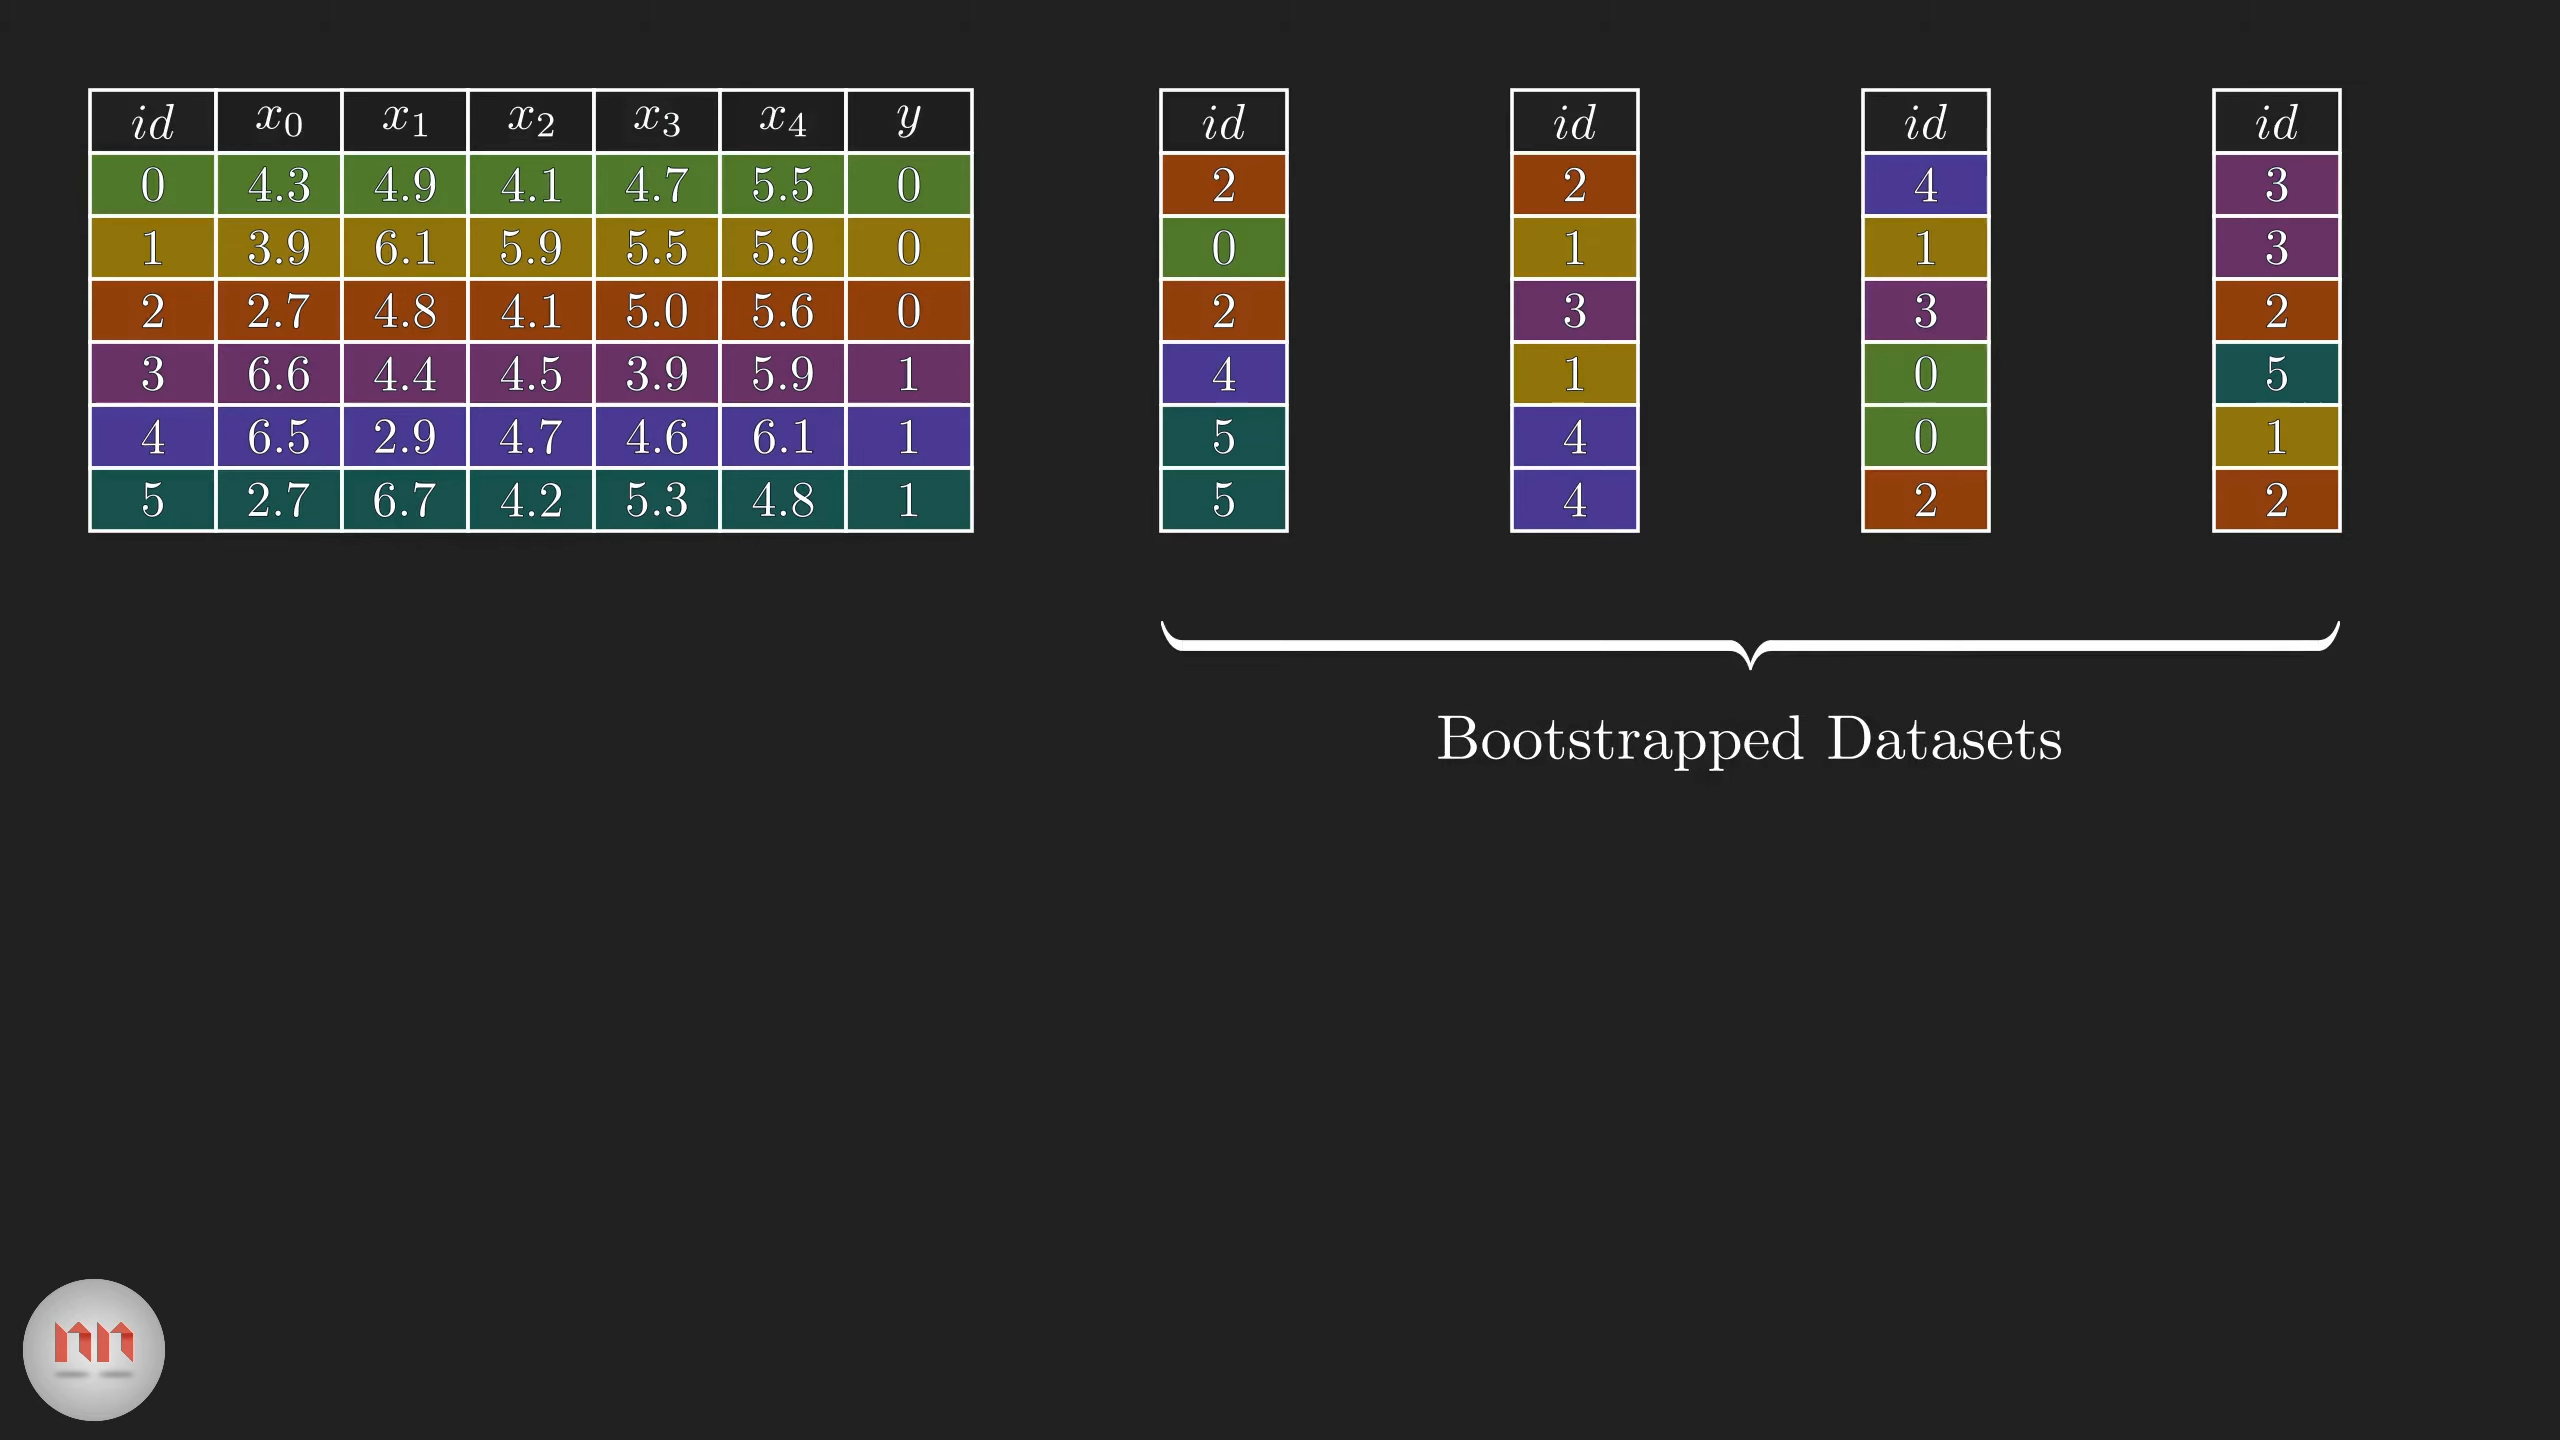
\includegraphics[width=13cm]{figs/rf/_3-30 screenshot.png}
{\tiny \href{https://www.youtube.com/watch?v=ZVR2Way4nwQ}{ \copyright Normalized Nerd}}
\end{frame}

\begin{frame}{Randomly select only 2 features for each dataset}
\hspace*{-1cm}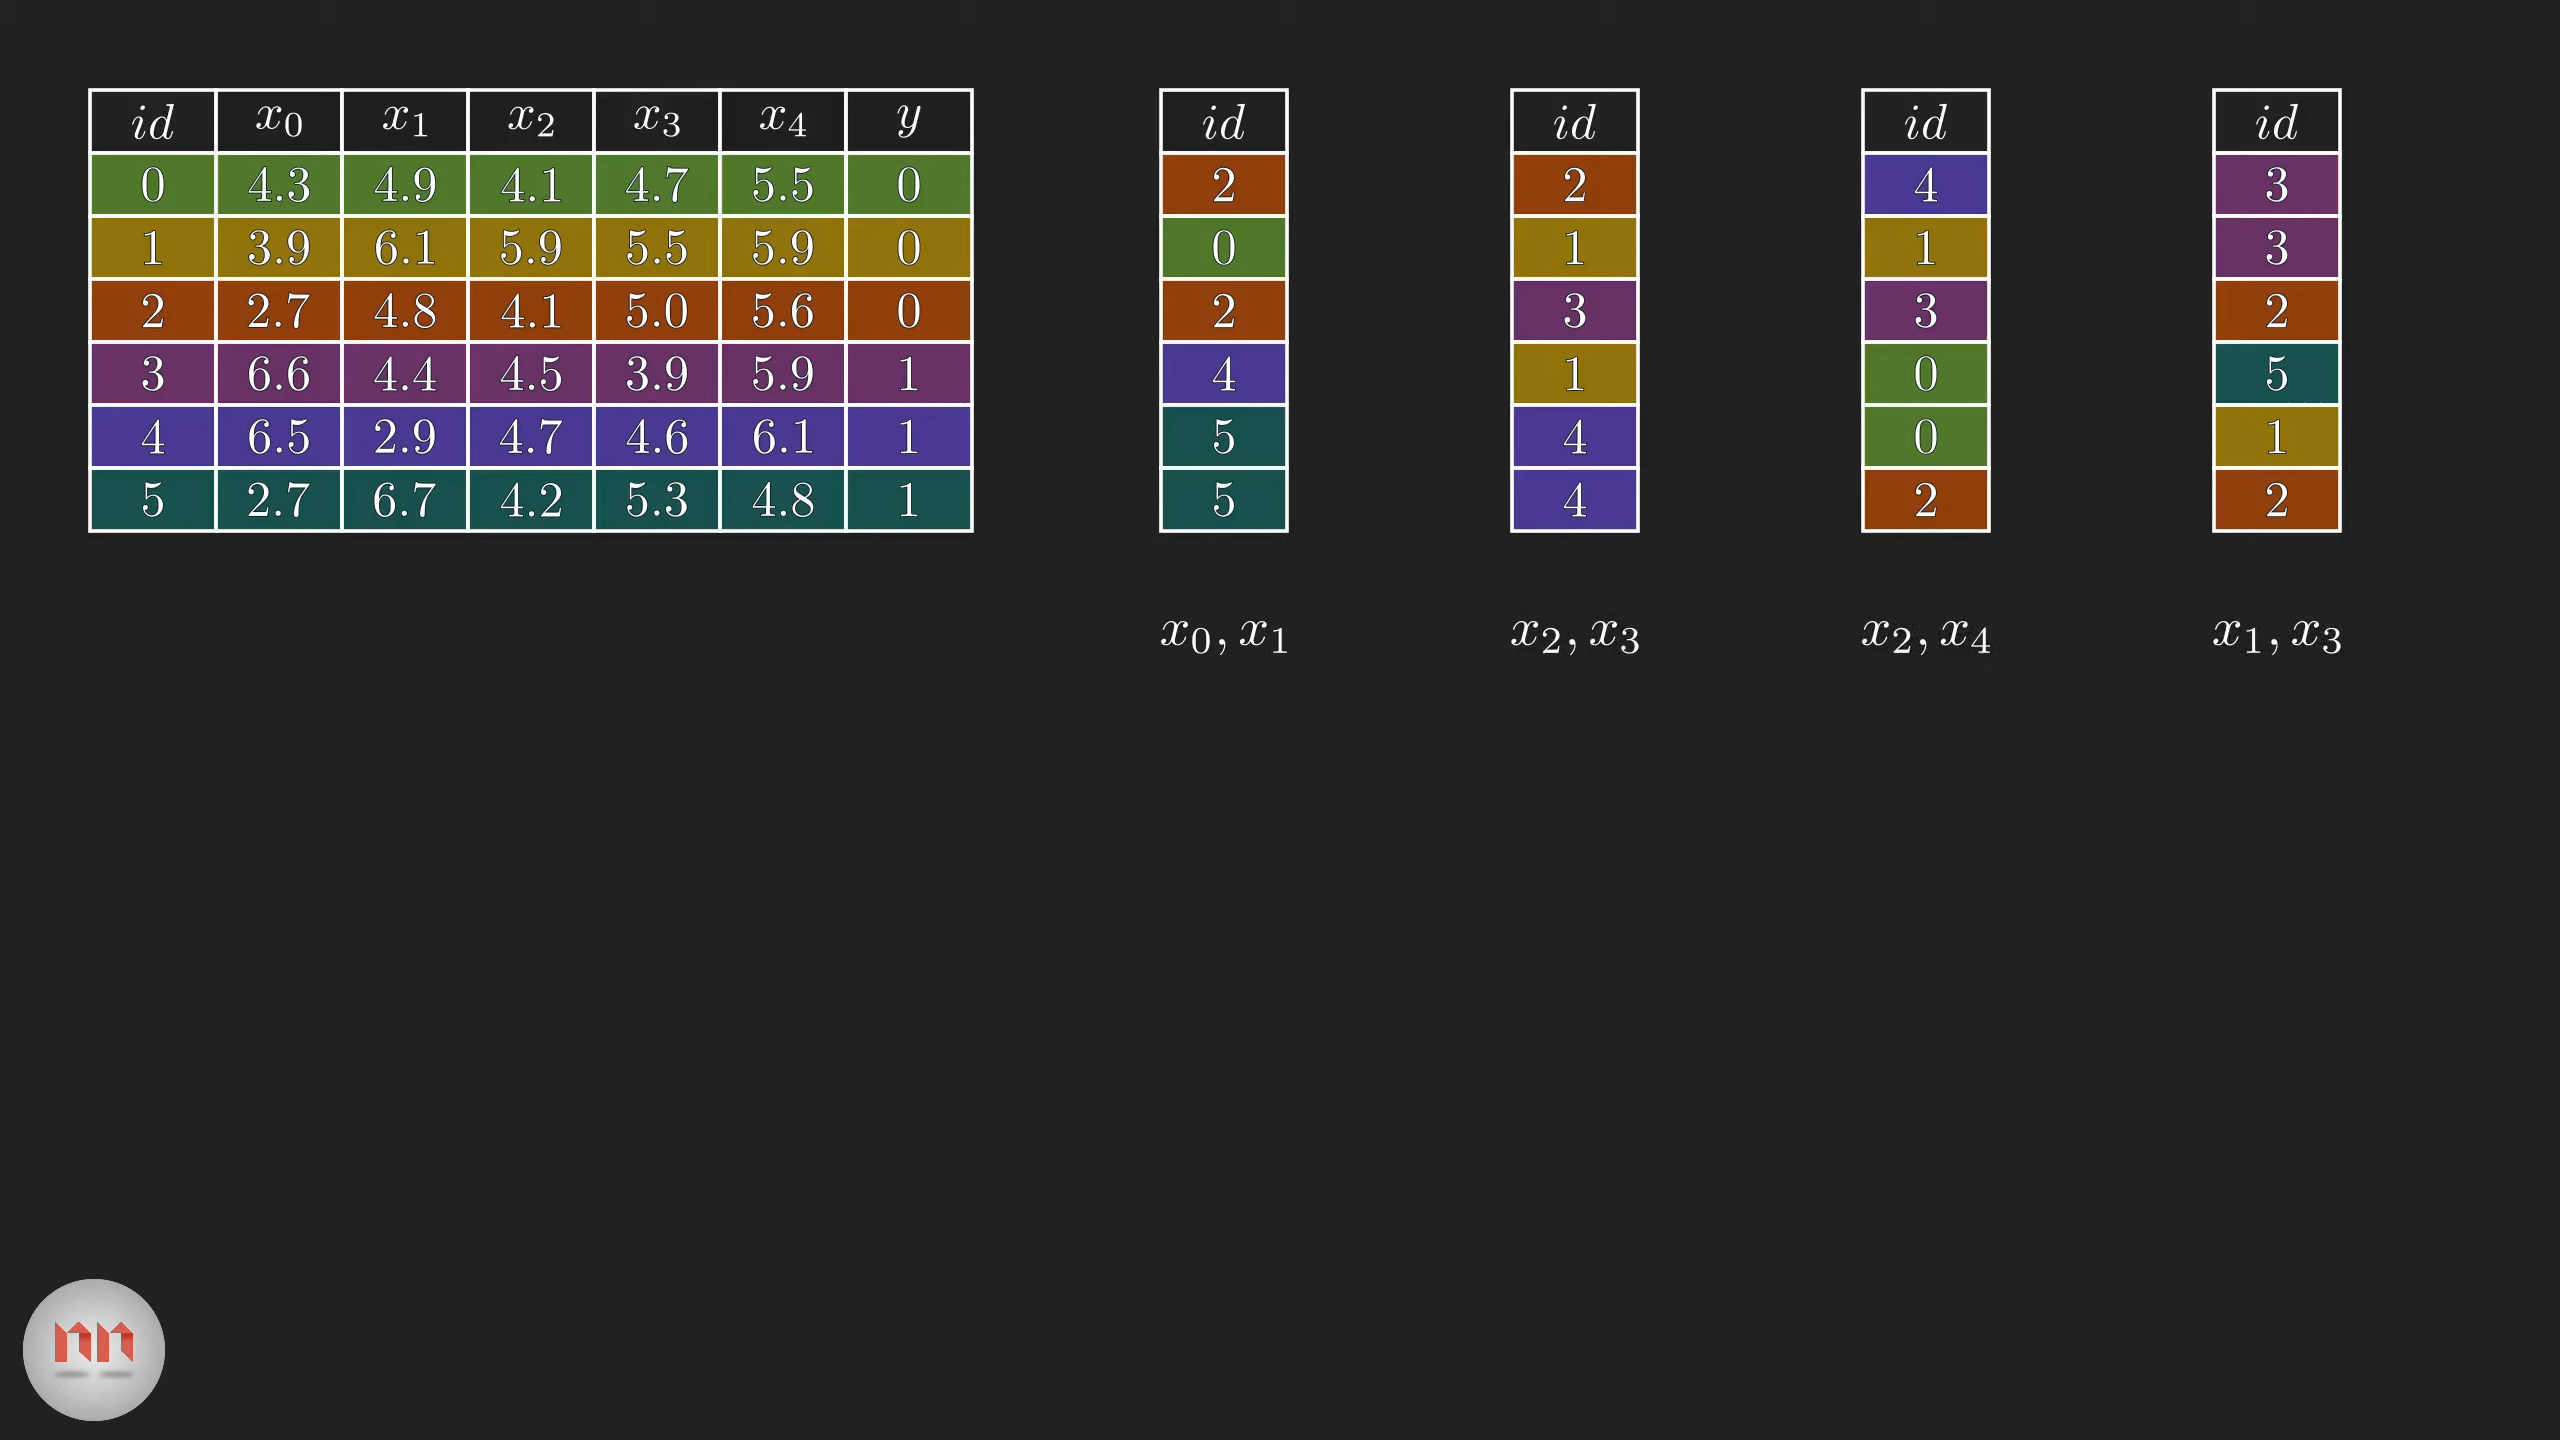
\includegraphics[width=13cm]{figs/rf/_4-2 screenshot.png}
{\tiny \href{https://www.youtube.com/watch?v=ZVR2Way4nwQ}{ \copyright Normalized Nerd}}
\end{frame}

\begin{frame}{Build decision trees for each dataset}
\hspace*{-1cm}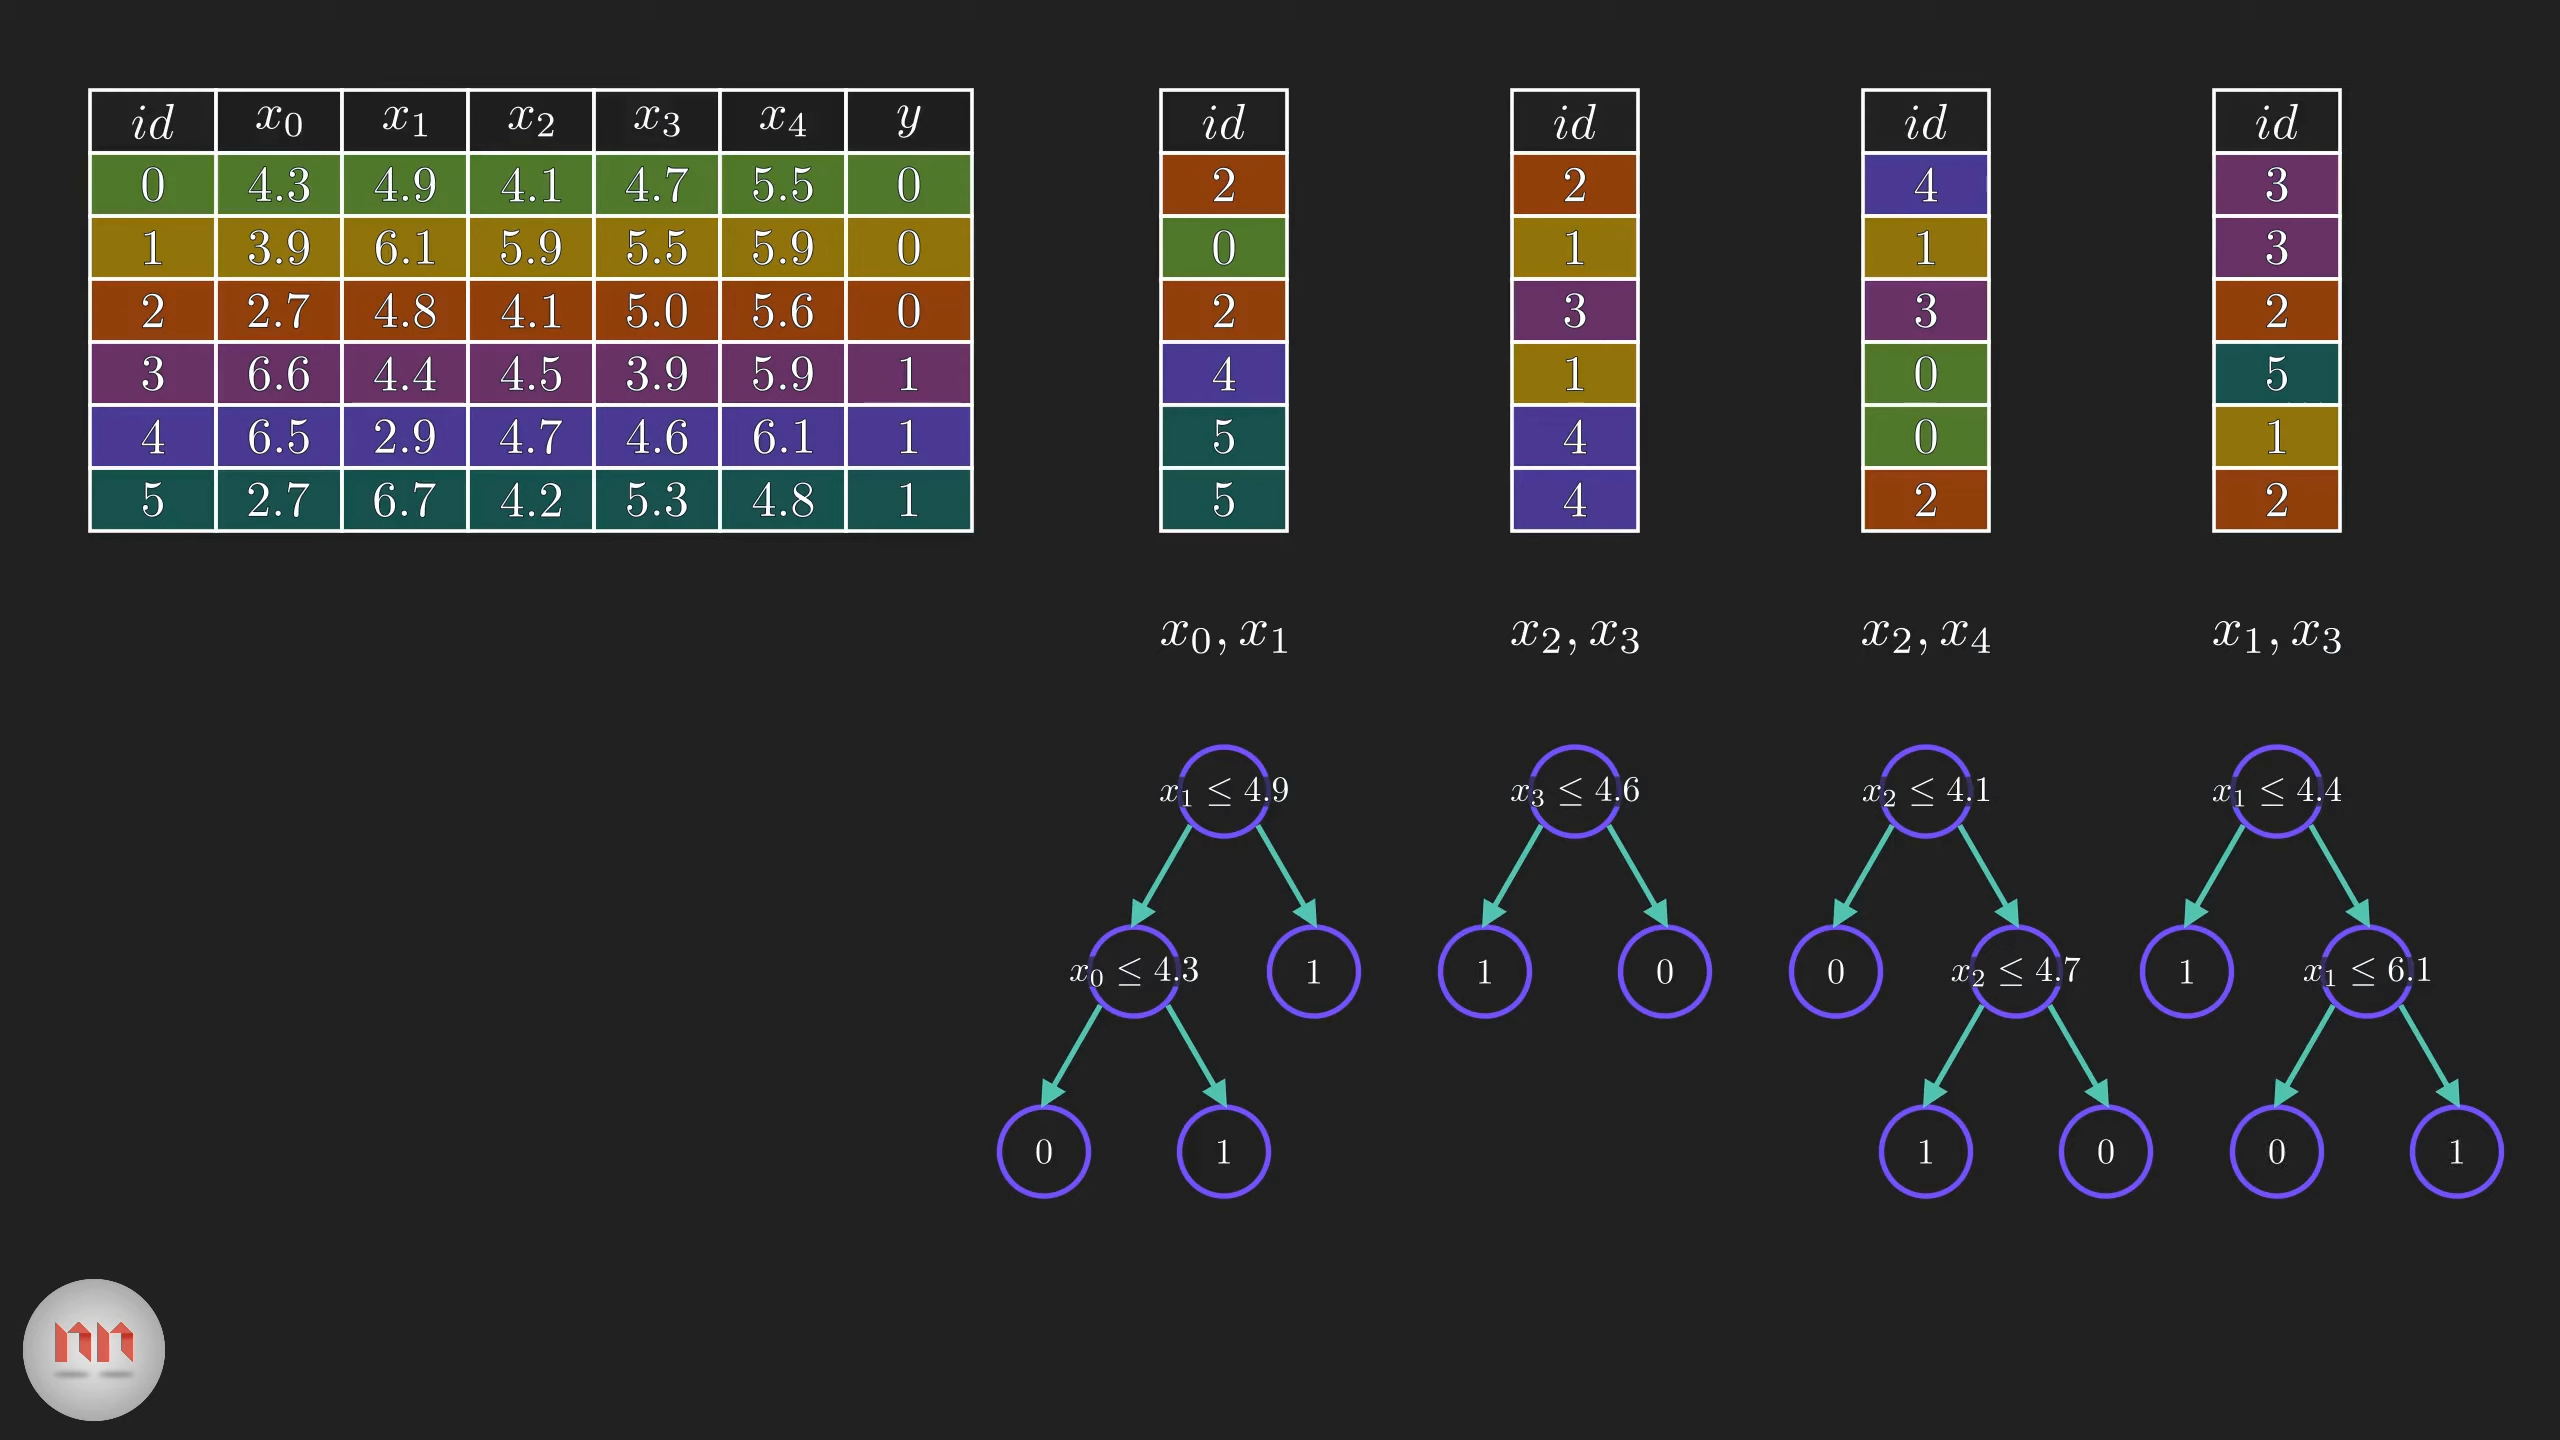
\includegraphics[width=13cm]{figs/rf/_4-35 screenshot.png}
{\tiny \href{https://www.youtube.com/watch?v=ZVR2Way4nwQ}{ \copyright Normalized Nerd}}
\end{frame}

\begin{frame}{A new point}
\hspace*{-1cm}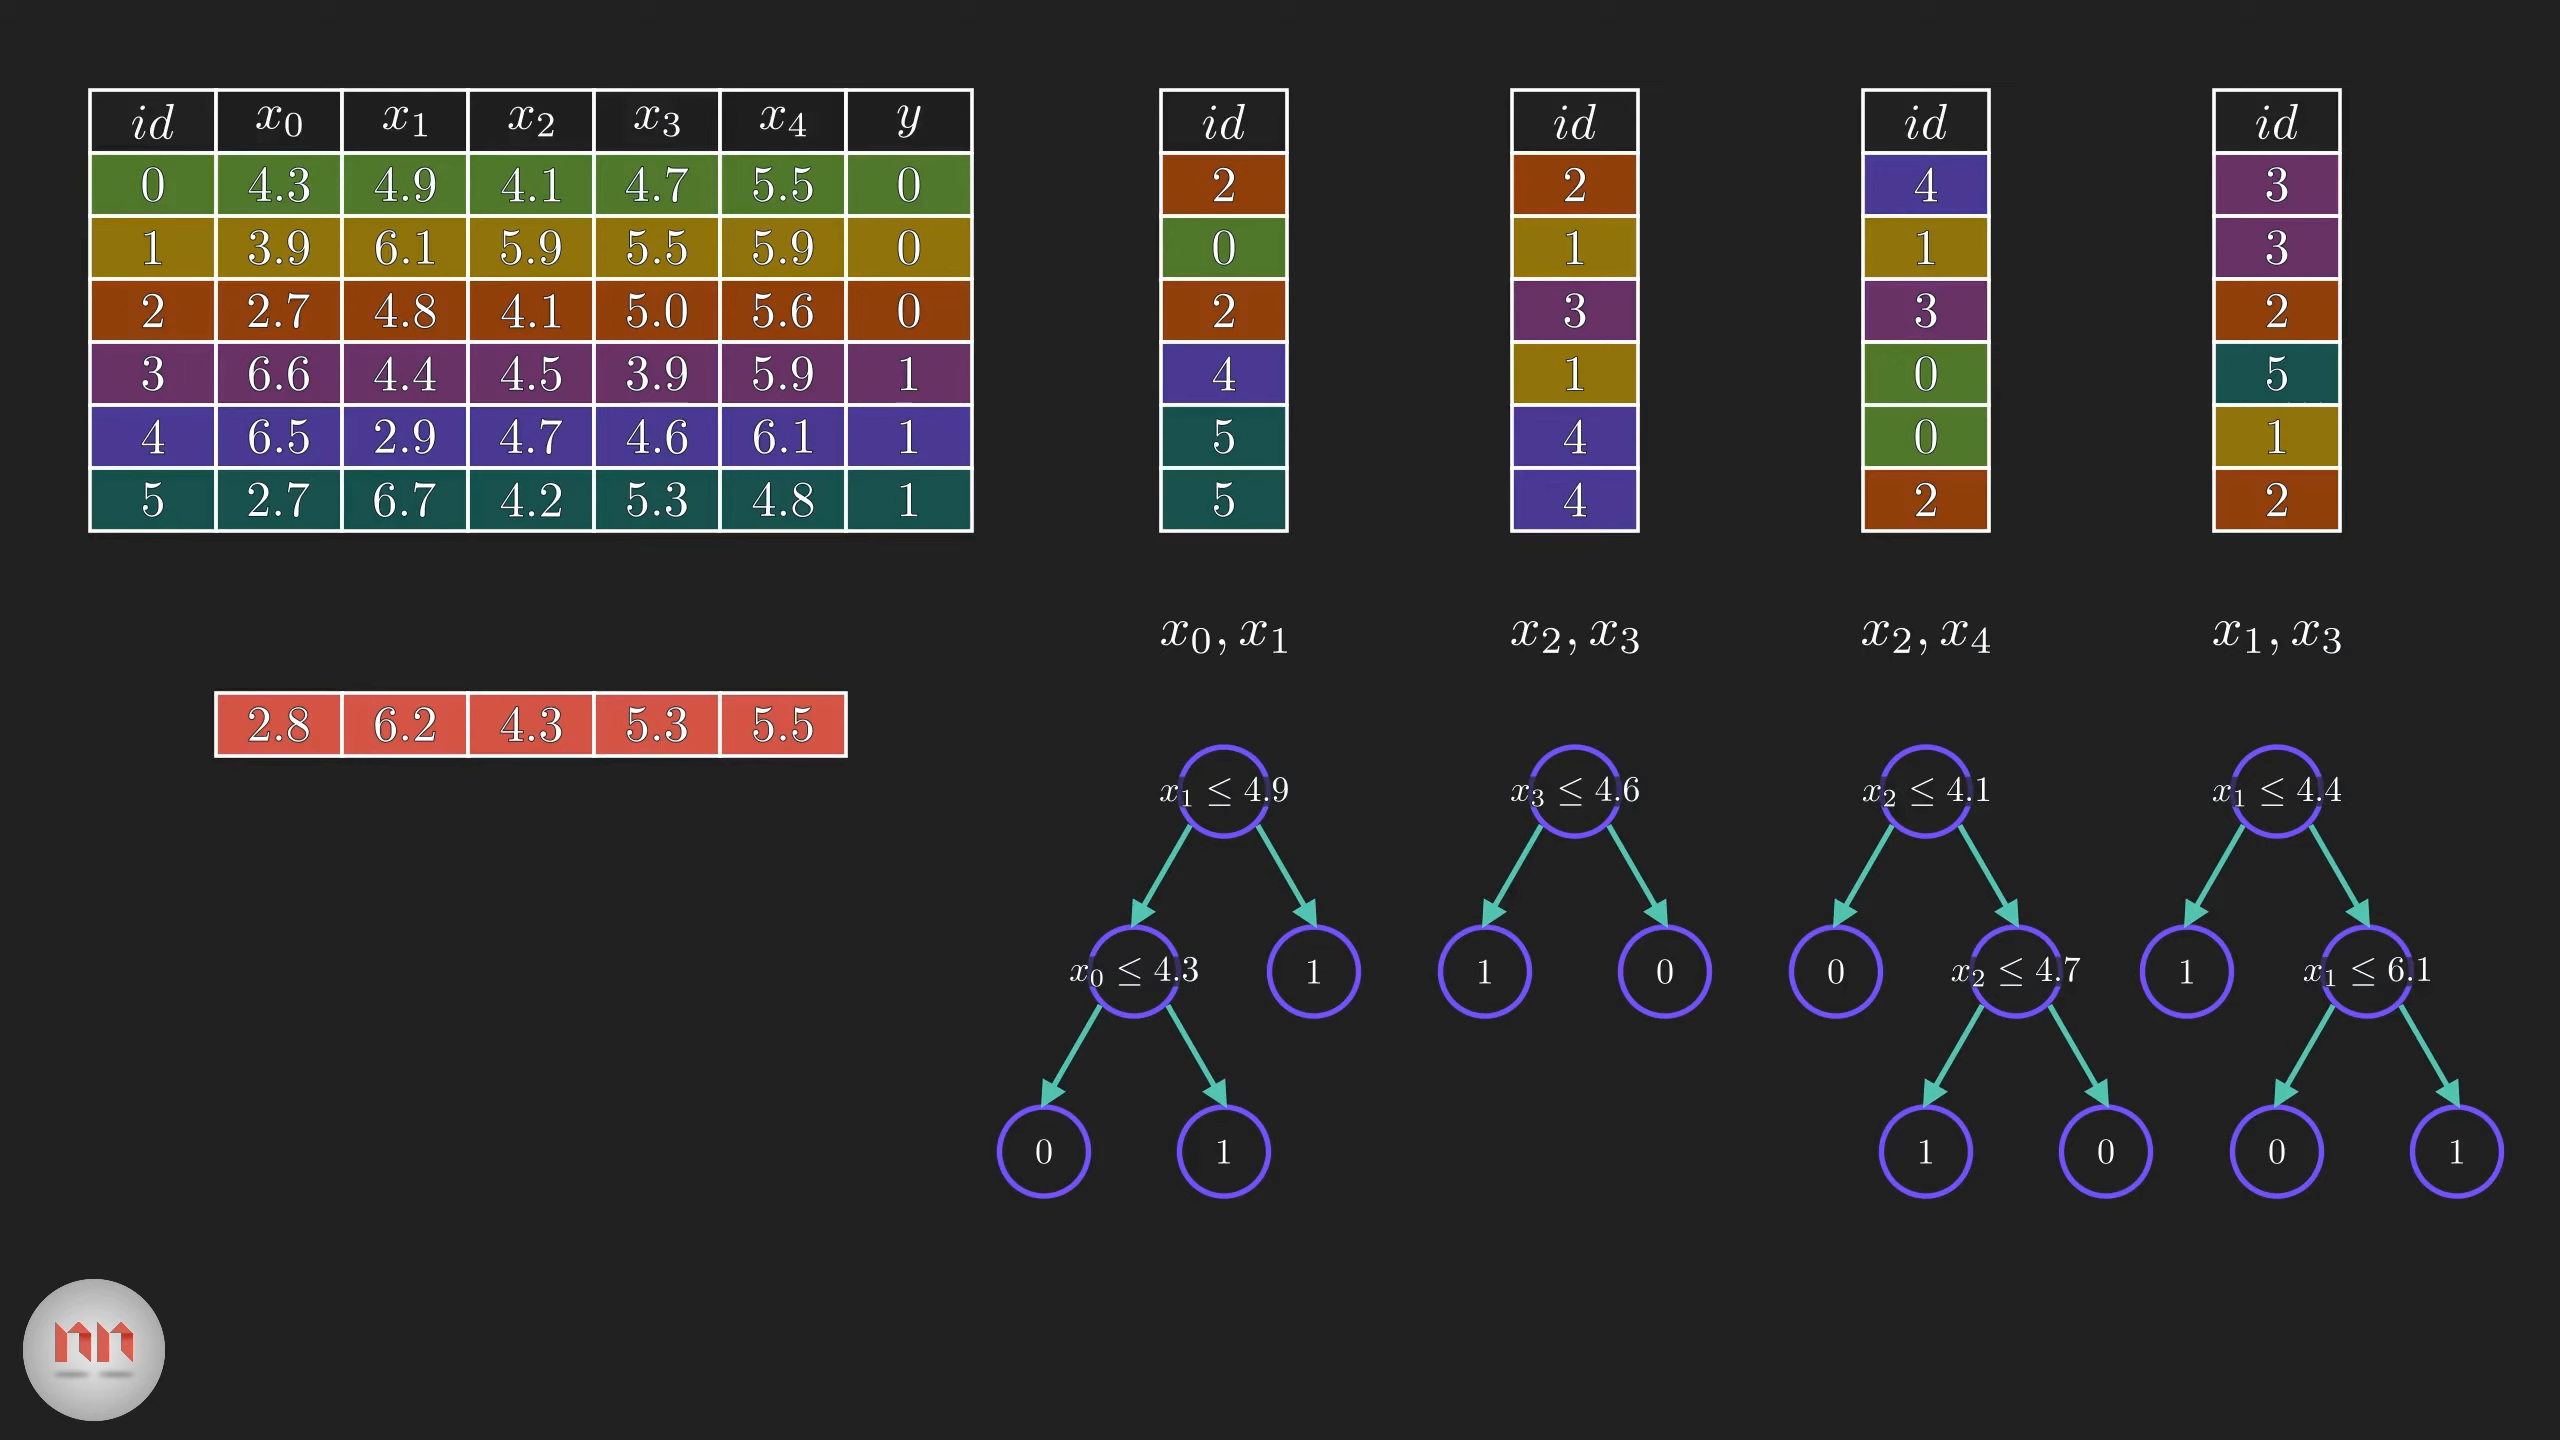
\includegraphics[width=13cm]{figs/rf/_4-57 screenshot.png}
{\tiny \href{https://www.youtube.com/watch?v=ZVR2Way4nwQ}{ \copyright Normalized Nerd}}
\end{frame}

\begin{frame}{Apply the decision trees for the new point}
\hspace*{-1cm}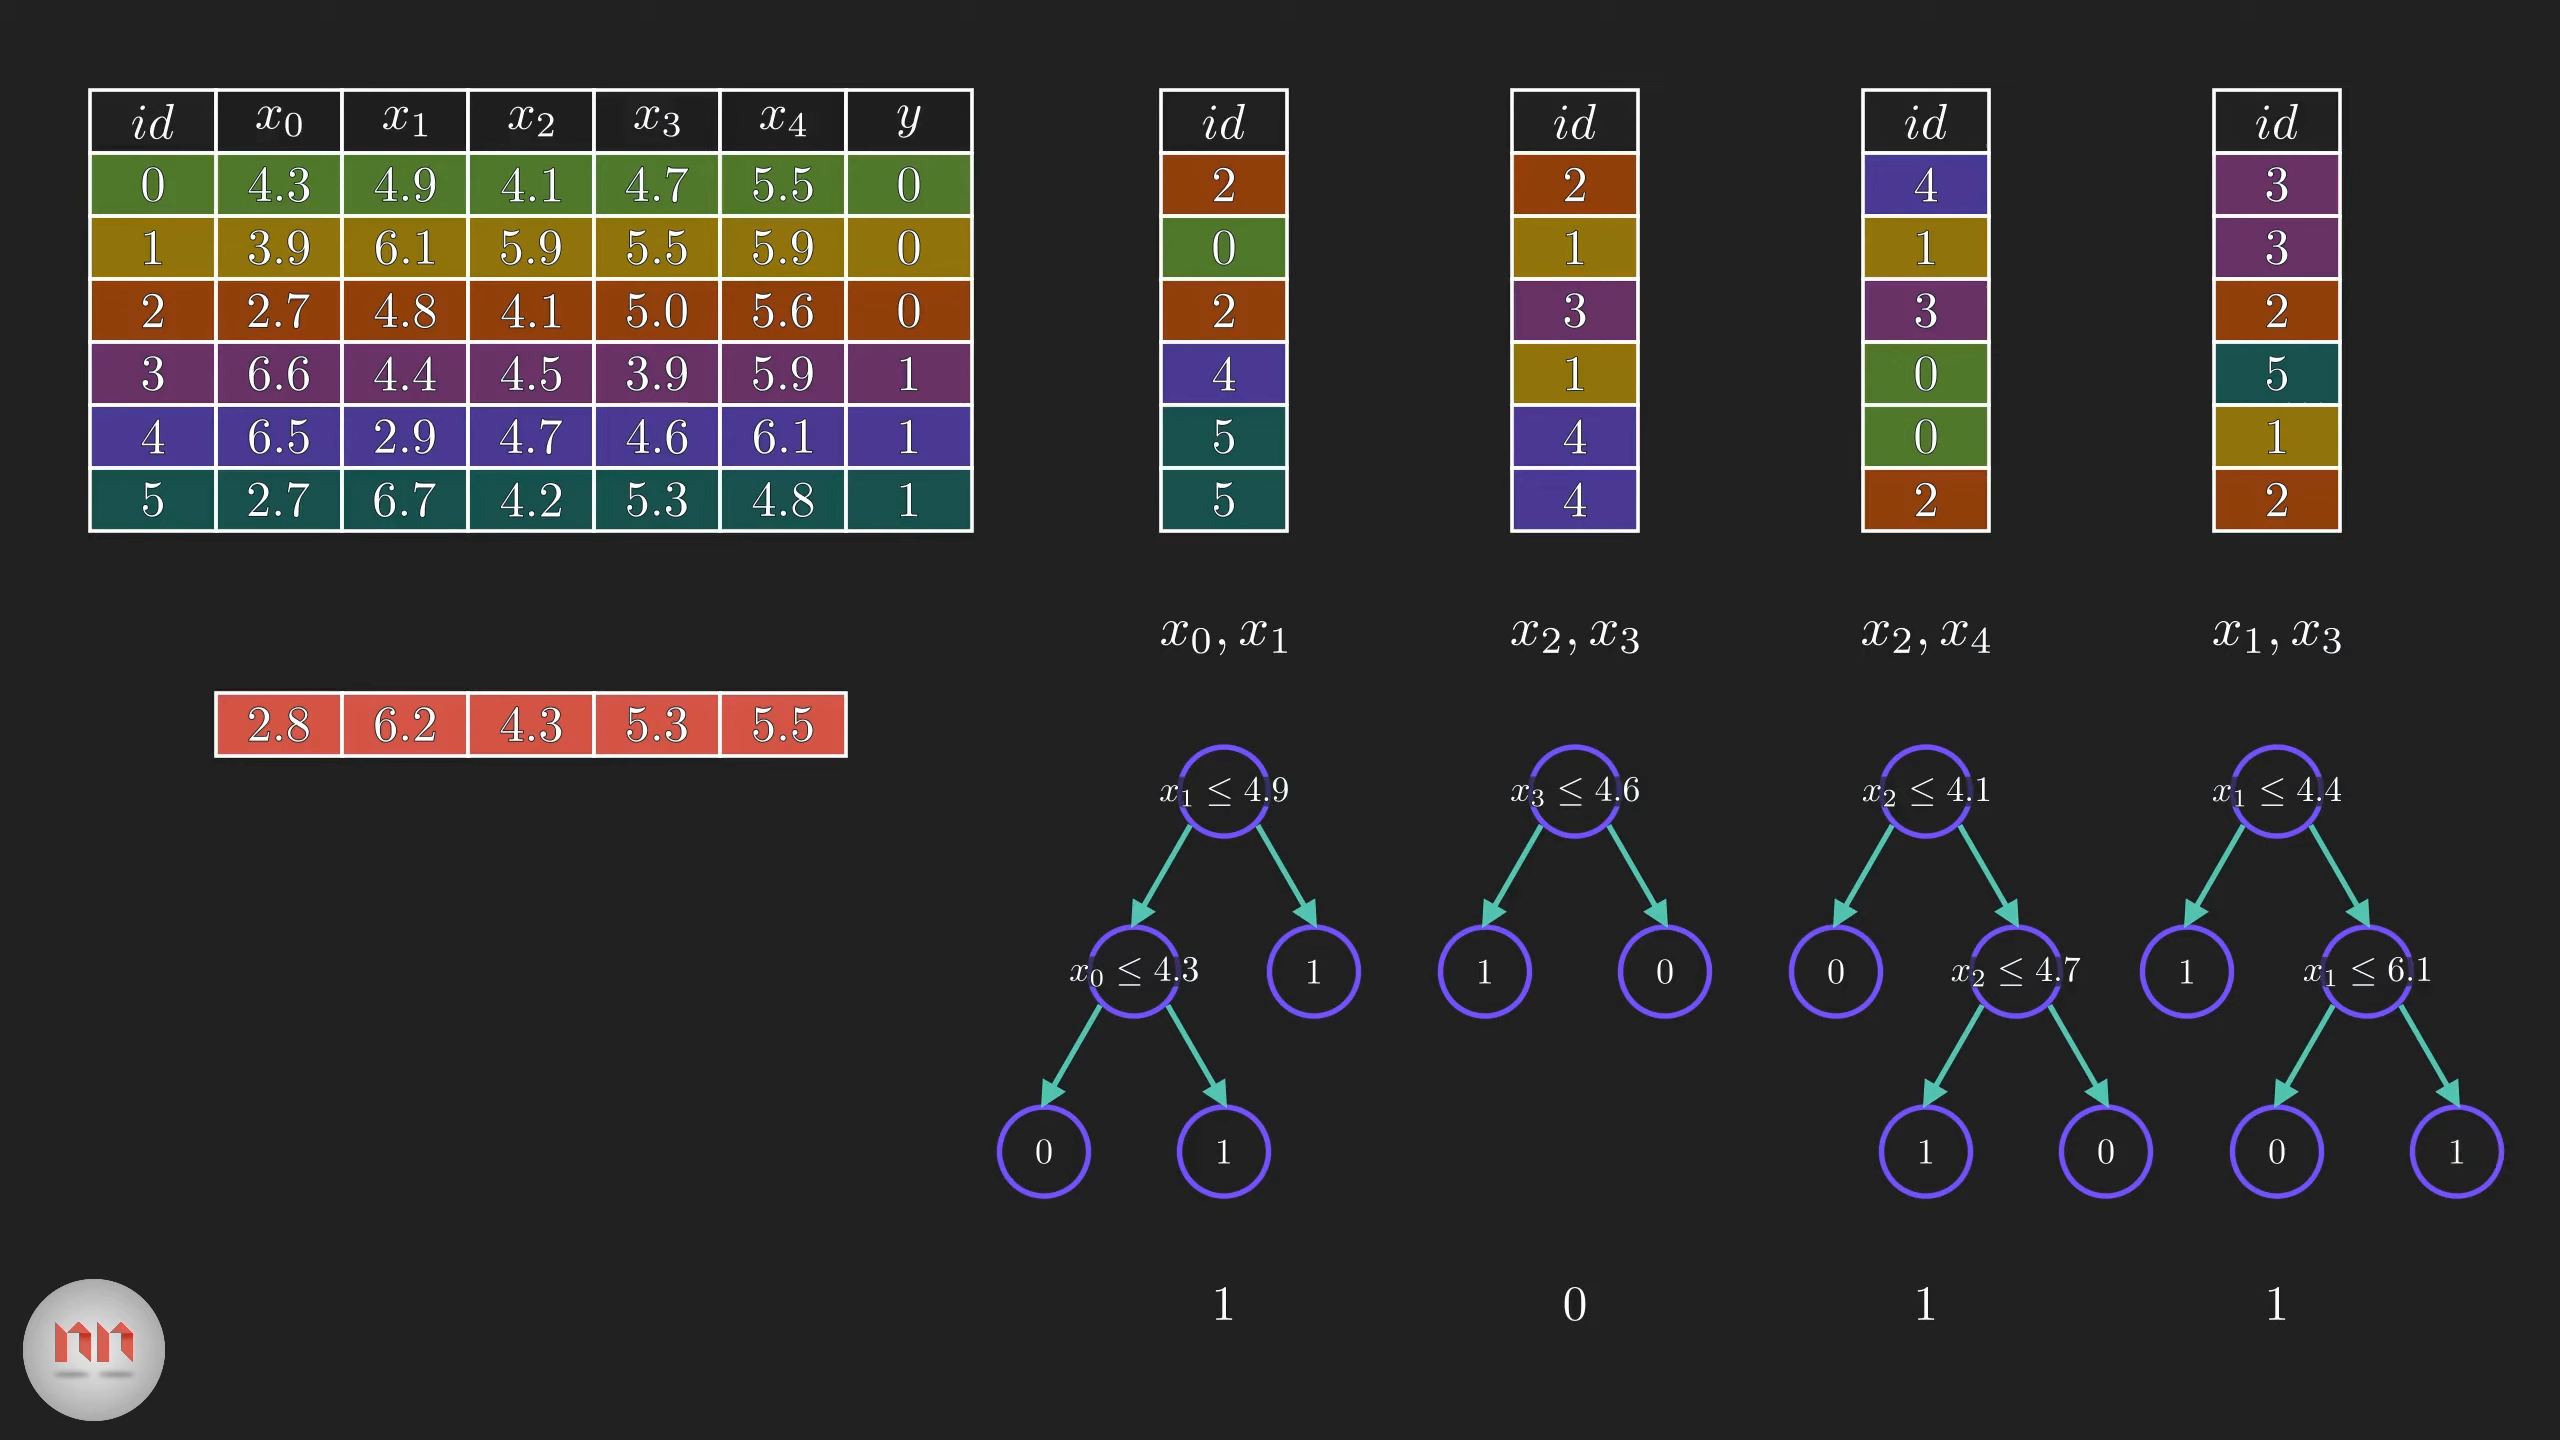
\includegraphics[width=13cm]{figs/rf/_5-23 screenshot.png}
{\tiny \href{https://www.youtube.com/watch?v=ZVR2Way4nwQ}{ \copyright Normalized Nerd}}
\end{frame}

\begin{frame}{Aggregate answers}
\hspace*{-1cm}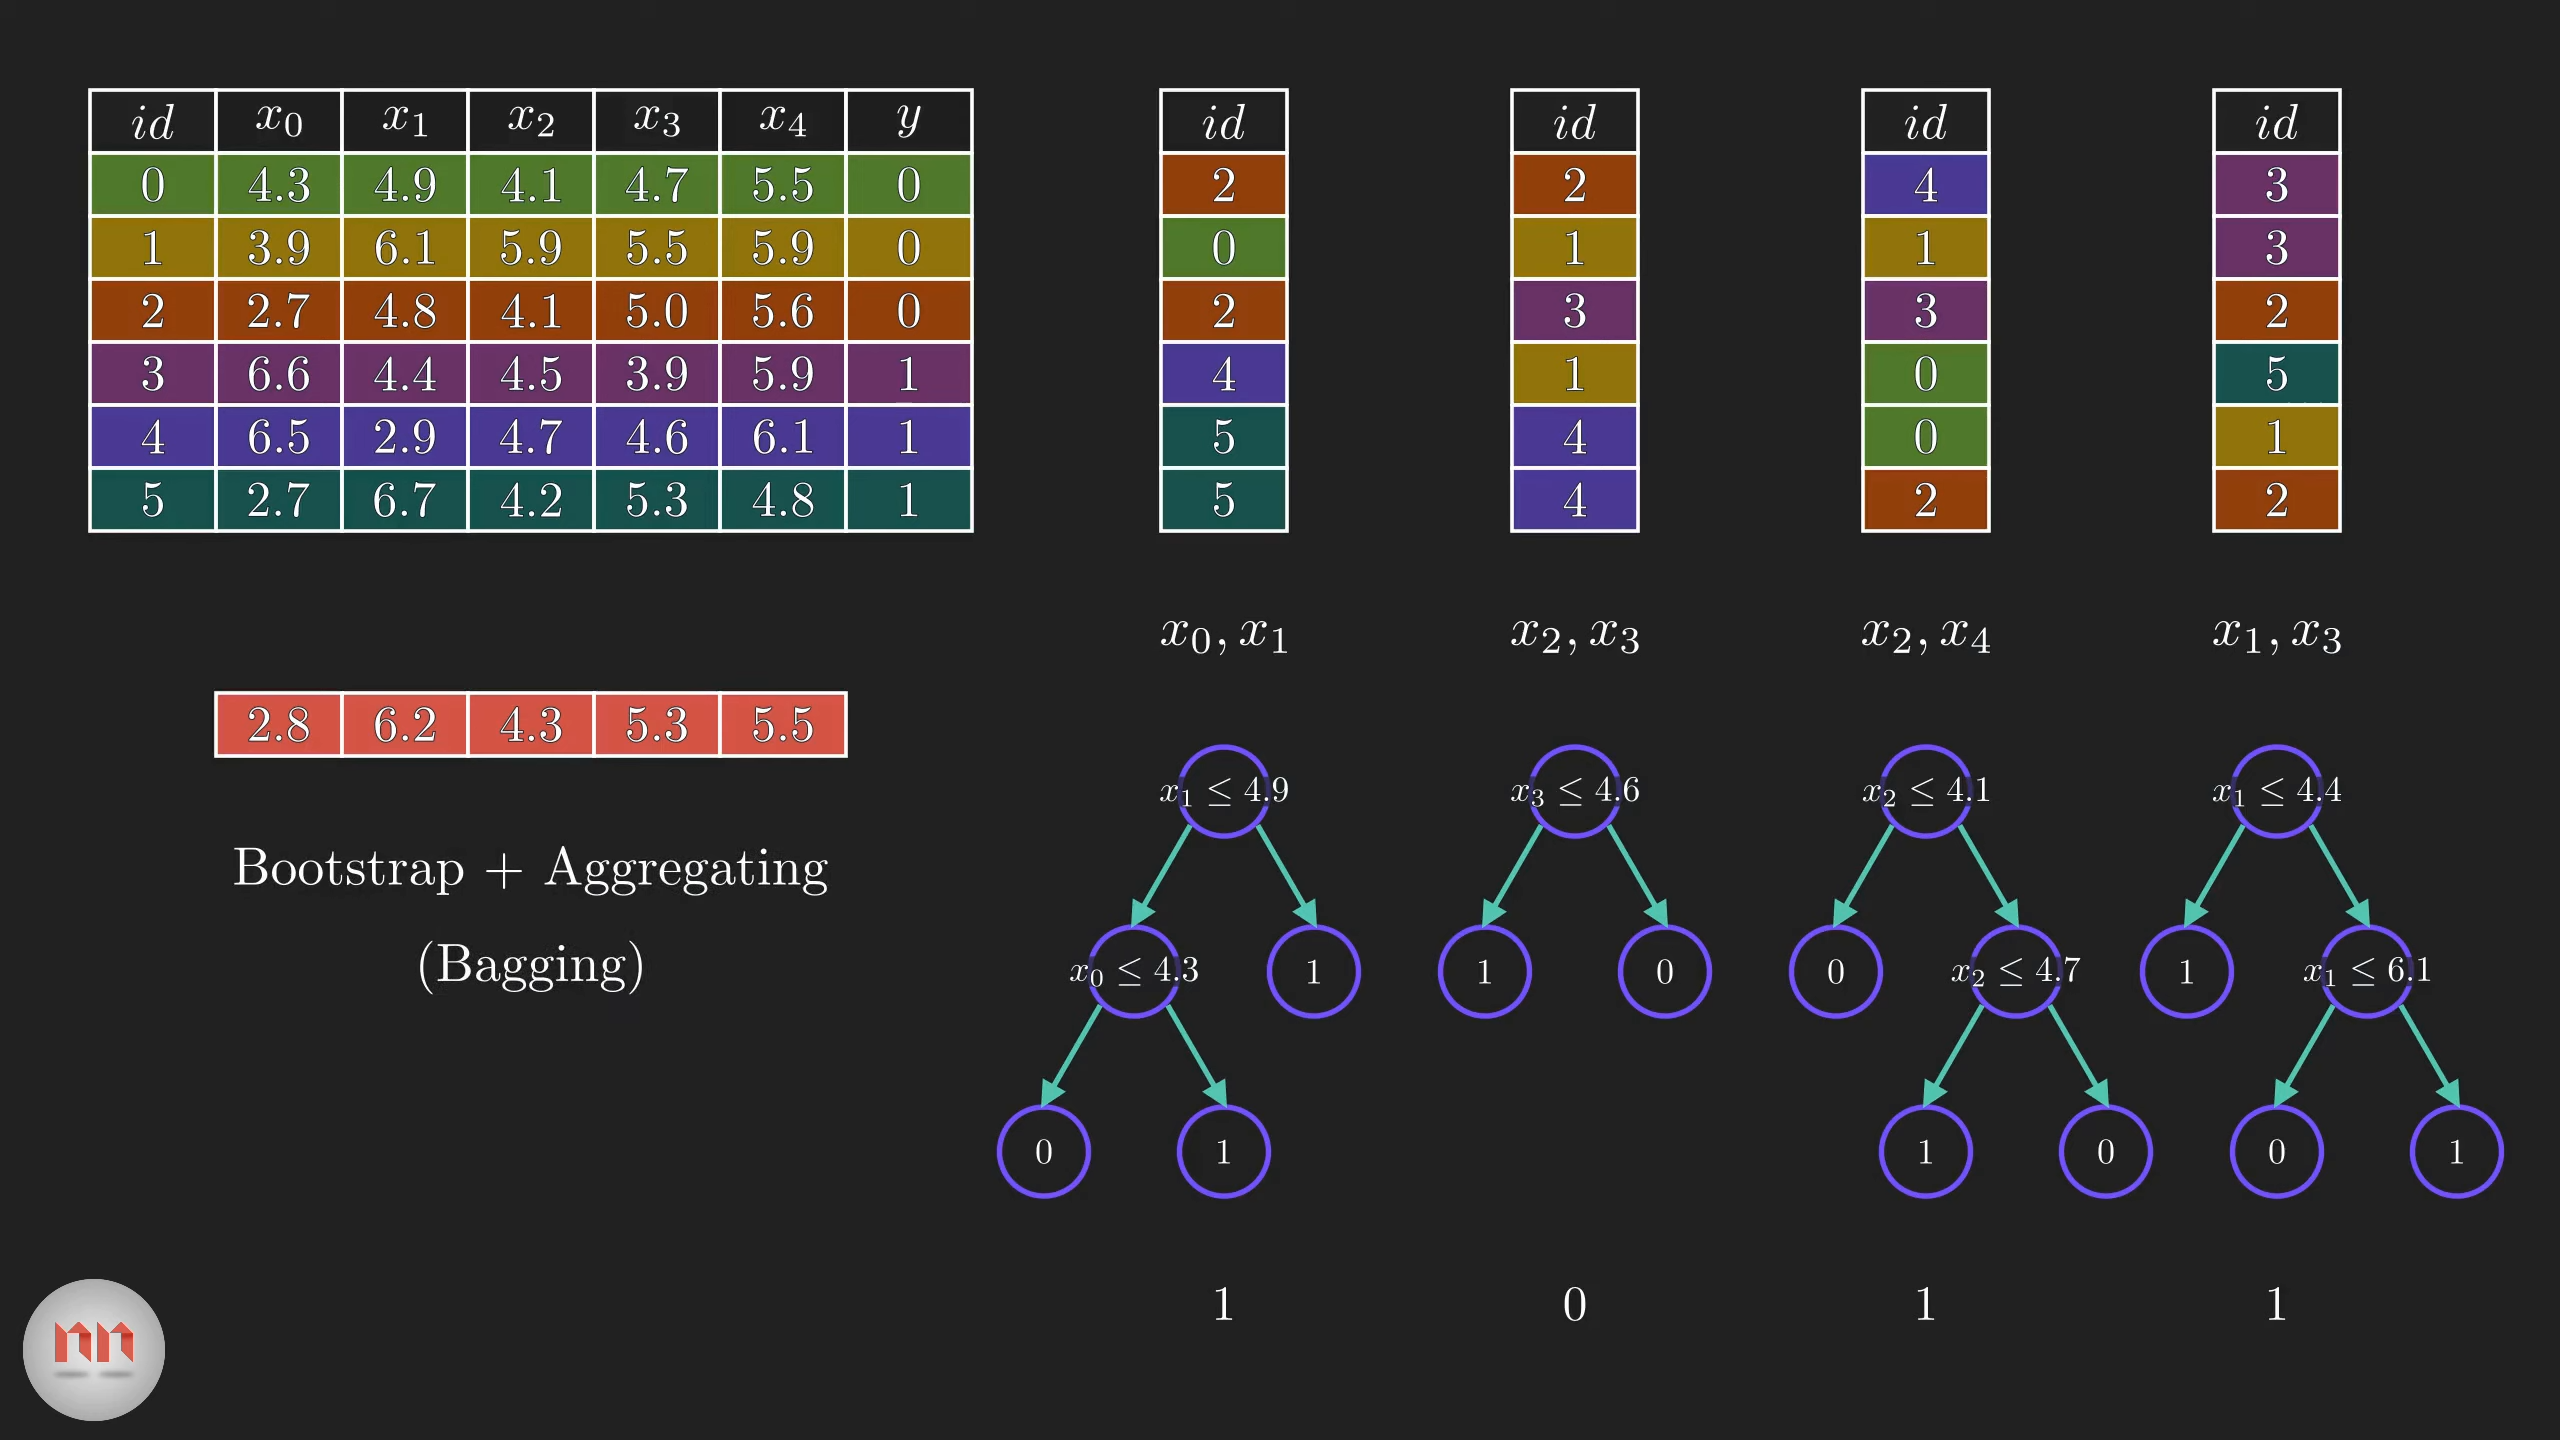
\includegraphics[width=13cm]{figs/rf/_5-48 screenshot.png}
{\tiny \href{https://www.youtube.com/watch?v=ZVR2Way4nwQ}{ \copyright Normalized Nerd}}
\end{frame}

\begin{frame}{Summary: random forest algorithm algorithm}
\begin{block}{Build a random forest}
\begin{itemize}
    \item Bootstrap the dataset
    \begin{itemize}
        \item Take $n$ random points from the dataset with repetition
        \item Take $m$ random features
        \item Create $k$ random datasets
    \end{itemize}
    \item Train K decision trees
\end{itemize}
\end{block}
\pause
\begin{block}{Apply the random forest}
\begin{itemize}
    \item Traverse the original dataset through K decision trees using $m$ features
    \item Aggregate results from each decision tree (average or maximum probability)
\end{itemize}
\end{block}
\end{frame}

\begin{frame}{Summary: random forest algorithm algorithm}
\begin{block}{Build a random forest}
\begin{itemize}
    \item Bootstrap the dataset
    \begin{itemize}
        \item Take $n$ random points from the dataset with repetition
        \item Take $m$ random features
        \item Create $k$ random datasets
    \end{itemize}
    \item Train K decision trees
\end{itemize}
\end{block}
\begin{block}{Apply the random forest}
\begin{itemize}
    \item Traverse the original dataset through K decision trees using $m$ features
    \item Aggregate results from each decision tree (average or maximum probability)
\end{itemize}
\end{block}
\begin{textblock*}{8cm}(3cm,1cm) % {block width} (coords)
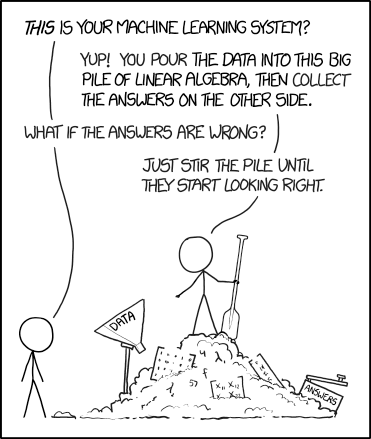
\includegraphics[width=7cm]{figs/machine_learning.png}
\end{textblock*}
\end{frame}

\section{Grid search}

\begin{frame}{Parameters and hyperparameters}
\begin{itemize}
    \item Parameters in the model that are optimized during training are called \alert{parameters} (e.g., the criteria on which we split the dataset into left and right sub-datasets)
\pause    
    \item Parameters that are not optimized during the training are called \alert{hyperparameters} (e.g., $k$ - number of decision trees in a random forest; $m$ - number of random features in each tree)
\pause    
    \item Hyperparameters can be determined using a score on the \alert{validation dataset} or using a \alert{cross-validation procedure}
\end{itemize}
\end{frame}

\begin{frame}{The grid search}
\begin{enumerate}
    \item Split the dataset into \alert{training} and \alert{validation} sub-datasets (e.g., with ratio 4:1)
    \item Specify a list of hyperparameters to be tested
    \item For each of the parameters, specify a set of values to test
    \item Train a model on the training sub-dataset for each of the possible combinations of hyperparameters
    \item Validate the model on the validation sub-dataset
    \item Retain the best model
\end{enumerate}
\end{frame}

\begin{frame}{Remarks on the grid search procedure}
\begin{itemize}
    \item It make an \alert{exhaustive} search of the hyperparameters
    \item The procedure is easy to \alert{parallelize}
    \item It is not naturally adapted for quantitative hyperparameters (not continuous).
    \item It can become \alert{very costly}. (e.g. 8 hyperparameters with 8 values each to test: $8^8$ = 16, 777, 216 trainings.
\end{itemize}
\end{frame}


\begin{frame}{The random search}
\begin{enumerate}
    \item Specify a list of hyperparameters to be tested
    \item For each of the parameters, specify a set of values to test or a law to draw a random value
    \item Draw $n$ combinations of the hyperparameters
    \item Train a model for each of the combinations and validate it on the validation sub-dataset
    \item Retain the best model
\end{enumerate}
\begin{figure}
    \centering
    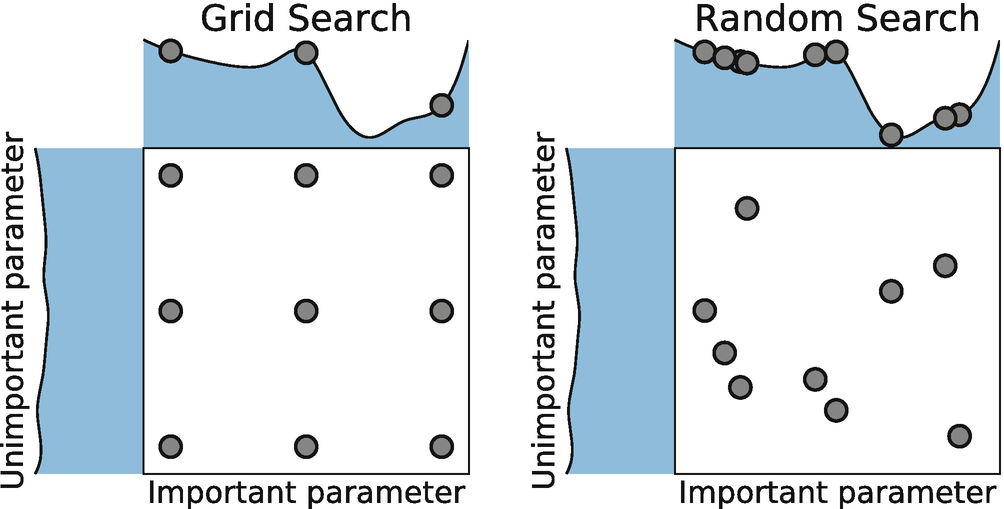
\includegraphics[width=.7\textwidth]{cIDuR2.png}
\end{figure}
\end{frame}

\begin{frame}{Remarks on the random search procedure}
\begin{itemize}
    \item It \alert{does not make} an \alert{exhaustive} search of the hyperparameters
    \item The procedure is easy to \alert{parallelize}.
    \item The cost is predictable (number of draw).
\end{itemize}
\pause
Both grid search and random search are implemented and easy to use in scikit-learn.
\end{frame}


\section{Data for the practical exercise}

\begin{frame}{AMSR2 passive microwave radiometer data}
\begin{itemize}
    \item Advanced Microwave Scanning Radiometer 2 (\alert{AMSR2}) 
    \item Measures \alert{brightness temperature} of the Earth surface at 7 frequencies and in 2 polarisations in Kelvins
    \item Fourteen 2D-arrays covering the Arctic (\alert{14 x 200 x 200} pixels)
    \item A subset from the original image with reduced resolution and coverage
\end{itemize}
\end{frame}

\begin{frame}{Sea ice type data}
\begin{itemize}
    \item Sea ice type product of the EUMETSAT OSI-SAF
    \item 3+1 type: Open water, First-year ice, Multi-year ice, Uncertain type
    \item Only one 2D-array covering the Arctic (\alert{200 x 200} pixels)
\end{itemize}
\pause
\hspace*{-1cm}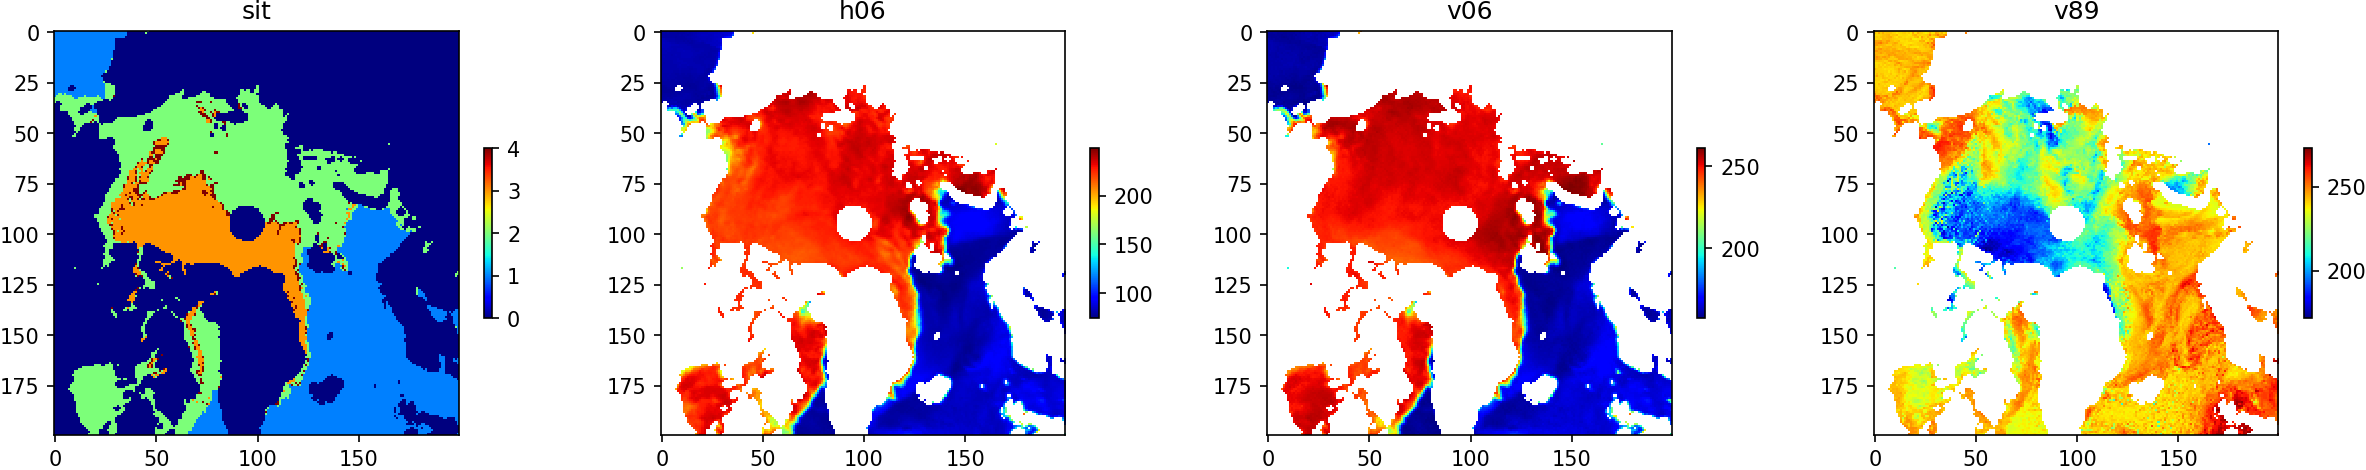
\includegraphics[width=13cm]{sit_amsr2_bands}
\tiny Aaboe, S., L.-A. Breivik and S. Eastwood (2014), Improvement of OSI SAF Product of Sea Ice Edge and Sea Ice Type. EUMETSAT Meteorological Satellite Conference, Geneva (Switzerland), September 2014.
\end{frame}

\end{document}